\documentclass[12pt]{report}
\usepackage[utf8]{inputenc}
\usepackage[T1]{fontenc}
\usepackage[english]{babel}
\usepackage{fourier}
\usepackage{expex}
\usepackage{pgfplots}
\usepackage{hyphenat}
\usepackage{tikz-qtree}
\usepackage{tikz}
\usetikzlibrary{calc}
\usepackage{avm}
\usepackage[normalem]{ulem}
\usepackage{amsmath}
\usepackage{amssymb}
\usepackage{amsthm}
\usepackage{ragged2e}
\usepackage{floatrow}
\usepackage{hyperref}
\usepackage{graphicx}
\usepackage{fancyhdr}
\usepackage{fancyvrb}
\usepackage{spverbatim}
\usepackage[toc,page]{appendix}
\usepackage{soul}
\usepackage[a4paper,width=140mm,top=25mm,bottom=25mm]{geometry}
\usepackage{listings}
\usepackage{footnote}
\usepackage{multirow}
\makesavenoteenv{tabular}
\makesavenoteenv{table}


%% Verbatim

\newtheorem{VerbatimText}{}

%% Table of contents depth
\setcounter{tocdepth}{2}

%% Fancy headers
\fancyhead{}
\fancyhead[L]{Coordination of Unlikes in Turkish}
\fancyhead[R]{Chapter \thechapter }
\fancyfoot{}
\fancyfoot[C]{\thepage}

% No links

\hypersetup{hidelinks}

% AVM Setup

\avmfont{\small\sc}
\avmsortfont{\small}


% Citations

\usepackage{natbib}


\begin{document}
	
	% Abstracts %
	
	\begin{titlepage}
	\begin{center}
		\vspace*{1.5cm}
		
		{\huge University of Warsaw}
		
		\vspace{0.1cm}
		{\Large Faculty of Psychology}
		
		\vspace{3.5cm}
		
		{\Large Berke Sensekerci} \\ Record book number: 400466
		
		\vspace{2cm}
		
		{\huge Coordination of Unlikes in Turkish}
		
		
		\vspace{3cm}
		
		{\large Master's thesis \\ in the field of Cognitive Science}
	\end{center}
	
	\vspace{2.5cm}
	
	\begin{flushright}
		The thesis was written under the supervision of \\
		prof. dr hab. Adam Przepiórkowski \\
		Faculty of Philosophy, University of Warsaw \\
		Institute of Computer Science, Polish Academy of Sciences	
	\end{flushright}
	
	\vspace{2.5cm}
	
	\begin{center}
		Warsaw, August 2023
	\end{center}	
\end{titlepage}
	\pagestyle{empty}
	\section*{Summary}
	\begin{sloppypar}
\begin{small}
Coordination is a grammatical structure where two or more linguistic elements are joined together, typically via elements called conjunctions. Despite its prevalence in natural languages, coordination remains poorly understood. One widely accepted view posits that the grammaticality of a coordinate structure depends on the coordinated elements (conjuncts) having the same grammatical properties, such as case and syntactic category. Although this view has been repeatedly questioned in the past, the debate still centers on limited data mainly from Polish and English. To further challenge the assumption that conjuncts must be alike, the present study introduces two types of novel empirical data from Turkish to the current debate: corpus examples and judgments of native speakers. 
	
The study hypothesizes that the grammaticality of coordinate structures in Turkish is contingent upon the grammatical function of the conjuncts, rather than their syntactic categories or cases. To investigate this hypothesis, a large web corpus of 3.3 billion words (Turkish Web 2012) was searched using tailored Corpus Query Language queries. This search yielded 137 instances of unlike category coordination and 51 instances of unlike case coordination. Notably, almost all extracted examples (with five exceptions) feature conjuncts with matching grammatical functions.
	
To assess the acceptability of different configurations of unlike category/case coordination, a formal acceptability judgment survey was conducted with 48 native speakers. Distinct sentence stimuli were rated on a 7-point Likert scale (from --3 to 3). An analysis of the results indicates that mismatching functions significantly affect the acceptability ratings, supporting the significance of grammatical function in coordination.
	
Finally, the observed empirical facts are formalized and analyzed within the framework of Lexical-Functional Grammar, adhering to the approach proposed by Przepiórkowski \& Patejuk (2021). To validate the analysis, a computational implementation was carried out using Xerox Linguistic Environment, a specialized platform for implementing grammars based on Lexical-Functional Grammar.
	
In conclusion, this thesis adds to the growing body of research challenging the widely assumed notion that conjuncts must be alike in their cases and categories. Moreover, the implications of this research extend to formal linguistics and grammar engineering.
\end{small}
\end{sloppypar}

	\section*{Key words}
	\begin{small}
\textit{Coordination of unlike categories, coordination of unlike cases, corpus linguistics, experimental syntax, Lexical-Functional Grammar, Turkish syntax, grammar engineering.}
\end{small}
\section*{The title of the thesis in Polish}
Koordynacja różnych kategorii i~przypadków gramatycznych w języku tureckim
	\newpage
	\pagestyle{empty}
	\section*{Streszczenie}
	\begin{sloppypar}
\begin{small}
Koordynacja to struktura gramatyczna, w której połączone są dwa lub więcej składników, zwykle za pomocą elementów zwanych spójnikami. Pomimo jej powszechności w językach naturalnych koordynacja pozostaje słabo zrozumiana. Jedna powszechnie akceptowana teoria zakłada, że gramatyczność koordynacji zależy od tego, czy skoordynowane elementy (koniunky) mają takie same cechy gramatyczne, przede wszystkim takie same przypadki i klasy morfosyntaktyczne. Chociaż teoria ta wielokrotnie była w przeszłości kwestionowana, debata wciąż koncentruje się na ograniczonych danych głównie z języka polskiego i angielskiego. W~celu pełniejszego podważenia założenia, że koniunkty muszą być składniowo podobne, niniejsze badanie wprowadza do debaty dwa rodzaje nowych danych empirycznych z języka tureckiego: autentyczne przykłady korpusowe i osądy rodzimych użytkowników języka.

Badanie zakłada, że gramatyczność koordynacji w~języku tureckim zależy od funkcji gramatycznej koniunktów, a nie od ich klas czy przypadków gramatycznych. Aby zbadać tę hipotezę, przeszukano duży korpus internetowy liczący 3,3 miliarda słów (Turkish Web 2012), używając odpowiednich zapytań w języku Corpus Query Language. W wyniku tego przeszukania uzyskano 137 przypadków koordynacji różnych klas oraz 51 przypadków koordynacji różnych przypadków. Warto zauważyć, że prawie wszystkie wydobyte przykłady (za wyjątkiem pięciu) zawierały koniunkty o zgodnych funkcjach gramatycznych.

Aby ocenić akceptowalność różnych konfiguracji koordynacji różnych klas i~przypadków, przeprowadzono formalne badanie akceptowalności z udziałem 48 rodzimych użytkowników języka tureckiego. Różne bodźce zdaniowe były oceniane na 7-stopniowej skali Likerta (od –3 do 3). Analiza wyników wskazuje, że niezgodność funkcji gramatycznych znacząco wpływa negatywnie na oceny akceptowalności, wspierając istotne znaczenie tożsamości funkcji gramatycznych – ale nie klas czy przypadków – w koordynacji.

Zaobserwowane fakty empiryczne zostały sformalizowane i zanalizowane w ramach teorii Lexical-Functional Grammar (LFG), zgodnie z podejściem zaproponowanym przez Przepiórkowskiego i Patejuk (2021). Aby zweryfikować analizę, przeprowadzono implementację obliczeniową przy użyciu środowiska Xerox Linguistic Environment, specjalistycznej platformy do implementacji gramatyk LFG.

Podsumowując, niniejsza praca dyplomowa przyczynia się do rosnącego zbioru badań kwestionujących powszechnie przyjmowaną tezę, że spójniki muszą być podobne pod względem przypadków i klas gramatycznych. % Ponadto implikacje tej pracy sięgają także do formalnej lingwistyki i inżynierii gramatycznej, oferując nowe perspektywy i możliwości dla przyszłych badań w tej dziedzinie.
\end{small}
\end{sloppypar}
	\section*{Słowa kluczowe}
	\begin{small}
\textit{Koordynacja różnych kategorii, koordynacja różnych przypadków, lingwistyka korpusowa, składnia eksperymentalna, Lexical-Functional Grammar, składnia języka tureckiego, inżynieria lingwistyczna.}
\end{small}
\section*{The title of the thesis in English}
Coordination of Unlikes in Turkish

	
	% ToC %
	
	\tableofcontents
	
	% Body % 
	
	\pagestyle{fancy}
	\chapter{Introduction} \label{ch:introduction}
	\section{Background}
\justifying

\textit{Coordination} refers to a grammatical structure wherein two or more linguistic elements are conjoined, typically through coordinating elements known as \textit{conjunctions}. These conjoined elements, referred to as \textit{conjuncts}, can be single words, phrases, or even complete sentences. Despite the ubiquity of coordination in natural languages, the syntactic and semantic characteristics of coordinate structures remain a topic of extensive debate within theoretical linguistics.
Within the context of the present thesis, the central aim is to undertake an empirical investigation and formal analysis of an atypical form of coordination, termed ``unlike coordination,'' in Turkish data. 

\begin{sloppypar}
Unlike coordination occurs when the coordinated elements do not align either in terms of their syntactic categories (i.e., ``coordination of unlike categories'') or in their grammatical cases (i.e., ``coordination of unlike cases''). Illustrative examples of unlike coordination can be seen in the examples in (\ref{ex0}). In the English sentence in (\ref{ex0a}), the elements conjoined by \textit{and} differ in their syntactic category since the first conjunct, \textit{a Republican}, is a noun phrase (NP) while the second conjunct, \textit{proud of it}, is an adjectival phrase (AdjP). The Polish example in (\ref{ex0b}), on the other hand, exemplifies unlike case coordination. In this instance, both conjuncts are NPs, but they differ with respect to the grammatical cases that they bear.
\end{sloppypar}

\pex[glspace=!1em,everygla={},everyglb={},aboveglbskip=-.15ex, interpartskip=15pt]
\label{ex0}
\a\label{ex0a}Pat is [a Republican]\textsubscript{NP} and [proud of it]\textsubscript{AdjP}. \trailingcitation{\citep[p.\ 117, ex.\ (2b)]{sagetal1985}}
\a\label{ex0b} \begingl
\gla Dajcie wina i ca\l{}\k{a} \'swini\k{e}!  //
\glb give wine.\textsc{gen} and whole.\textsc{acc} pig.\textsc{acc} //
\glft `Serve (some) wine and a whole pig!' \trailingcitation{\citep[p.\ 175, ex.\ (5.269)]{prze:99}} //
\endgl
\xe

It should be noted that unlike coordination is not exempt from constraints. Not all configurations of unlike coordination are valid, as exemplified by the ungrammatical sentence in (\ref{ex1c}). While each of the conjuncts in (\ref{ex1c}) retains grammaticality when considered individually in (\ref{ex1a}) and (\ref{ex1b}), respectively; their coordination, which is an unlike category coordination (prepositional phrase (PP) \& complementizer phrase (CP)), yields an ungrammatical sentence. 

\pex
\label{ex1}
\a\label{ex1a}The scene [of the movie]\textsubscript{PP} was in Chicago.
\a\label{ex1b}The scene [that I wrote]\textsubscript{CP} was in Chicago. \trailingcitation{\citep[p.\ 36, ex.\ (24)]{Chomsky57}} 
\a\label{ex1c}\ljudge{*}The scene [of the movie]\textsubscript{PP} and [that I wrote]\textsubscript{CP} was in Chicago.
\trailingcitation{\citep[p.\ 36, ex.\ (25)]{Chomsky57}} 
\xe

\subsection{The law of the coordination of likes}
Unlike coordination (both of categories and cases) has been widely assumed to be impossible since as early as \citet[pp.\ 35--36]{Chomsky57}, where he concludes, on the basis of the examples in (\ref{ex1}), that conjuncts must not only qualify as constituents, as in (\ref{ex1a}) and (\ref{ex1b}), but also have the same category, as evinced by the ungrammaticality of (\ref{ex1c}). This generalization, which is commonly called the Law of the Coordination of the Likes (LCL; \citealp{Wiliams1981}), proved to be one of the well-entrenched views on the syntax of coordination even though contrary evidence started to appear as early as \citet{dik1968} and \citet{peterson1981}. Although the influence of this view is most pronounced in the early research on coordination within the transformational tradition \citep{schachter1977, Wiliams1981}, it still garners support from some researchers.\footnote{A recent defense of the LCL can be found in \citet{Bruening2020}.}

One of the commonly adopted strategies to maintain LCL in the face of contrary data has been to assume an intermediary elliptical process. This approach suggests that unlike coordination arises through the omission of specific elements from the underlying like coordination present in the base-generated sentence. Following this assumption, the unlike category coordination in (\ref{ex2b}), \textit{a plumber and making a fortune}, is a result of the elision of the repeated element from the second conjunct in the underlying like coordination in (\ref{ex2a}), which is the verb \textit{be}.

\pex 
\label{ex2}
\a\label{ex2a}Bill could be a plumber and be making a fortune.
\a\label{ex2b}Bill could be a plumber and $\varnothing$ making a fortune. \trailingcitation{\citep[p.\ 54, ex.\ (12a)]{beavers-sag:2004}} 
\xe

One far-reaching consequence of this analysis is that it renders the surface unlike coordination in (\ref{ex2b}), \textit{a plumber and making a fortune}, a non-constituent. In other words, there is no superior node that governs the entire coordinate structure. \citet{peterson2004}, however, refutes this consequence of ellipsis-based analysis by demonstrating that the surface unlike coordination must be regarded as a constituent based on some widely assumed tests of constituency. These tests include topicalization, as illustrated in (\ref{ex3a}), pro-form \textit{so} substitution, as seen in (\ref{ex3b}), and right node raising, as exemplified in (\ref{ex3c}). Therefore, the phenomenon of unlike coordination cannot be explained away by adopting an ellipsis-based analysis.

\pex
\label{ex3}
\a\label{ex3a}A plumber and making a fortune though Bill may be, he's not
going to be invited to my party. \trailingcitation{\citep[p.\ 648, ex.\ (10a)]{peterson2004}}
\a\label{ex3b}Bill is a plumber and making a fortune, and so is John. \trailingcitation{\citep[p.\ 648, ex.\ (11a)]{peterson2004}}
\a\label{ex3c}Bill is, and John soon will be, a master plumber and making a
fortune. \trailingcitation{\citep[p.\ 649, ex.\ (12a)]{peterson2004}}
\xe

\subsection{Alternative accounts of unlike coordination}
In non-transformational frameworks, such as GPSG\footnote{Generalized Phrase Structure Grammar; \citealp{gazdaretal1985}}, HPSG\footnote{Head-Driven Phrase Structure Grammar; \citealp{pollardetal1994, muller:2021}} and LFG\footnote{Lexical-Functional Grammar; \citealp{kaplan&bresnan_1982, Dalrymple2019}}, unlike coordination has been acknowledged as a genuine case of coordination, and various analyses to account for its behavior have been offered.

\subsubsection{Sag et al. (1985)}
\citeauthor{sagetal1985}'s \citeyearpar{sagetal1985} GPSG analysis of unlike coordination constituted one of the first systematic attempts at formally modeling the phenomenon in question. In their analysis, the sentence (\ref{ex4a}) is grammatical because the individual conjuncts meet the only requirement set by the verb \textsc{become}: they are predicative arguments of the verb. Since \textsc{become} does not impose any constraint regarding the syntactic category of its predicative argument, unlike category coordination becomes possible as long as the individual conjuncts fulfill the external requirements imposed on them. In this line of reasoning, the ungrammaticality of (\ref{ex4b}) can also be explained since the individual conjuncts fail to satisfy the more specific constraints imposed by \textsc{become}. Namely, the conjuncts in the argument position should not only be predicative elements but also either nominals or adjectivals. This grammatical relation between the verb and its coordinated arguments is established through the mother node immediately dominating the conjuncts, which bears only the features that are common to all conjuncts.\footnote{The formal details behind \citeauthor{sagetal1985}'s GPSG analysis are grossly simplified here, as a detailed treatment of their analysis is beyond the scope of the present chapter.} 

\pex
\label{ex4}
\a\label{ex4a}Pat became a Republican and quite conservative. \trailingcitation{\citep[p.\ 142, ex.\ (67a)]{sagetal1985}}
\a\label{ex4b}\ljudge{*}Tracy has become a Republican and of the opinion that we
must place nuclear weapons in Europe. \trailingcitation{\citep[p.\ 142, ex.\ (67b)]{sagetal1985}}
\xe

\subsubsection{Bayer (1996)}
\citeauthor{sagetal1985}'s (\citeyear{sagetal1985}) work demonstrated that there is no intrinsic categorial constraint imposed upon the conjuncts by the coordination itself. The constraints on coordinate structures can instead be explained and modeled in terms of more fundamental syntactic relations between the coordination and its external governor. \citeauthor{sagetal1985}'s (\citeyear{sagetal1985}) analysis, however, was driven primarily by English data and, as a consequence, effectively only dealt with unlike category coordination in complement position. 

The analysis proposed by \citet{bayer1996} frames the phenomenon solely as a relationship between individual conjuncts and their external governor. Under his analysis, syntactic constraints are encoded strictly in terms of disjunctive or conjunctive statements that are, in effect, evaluated for each conjunct. For instance, \textsc{become} specifies that its predicative complement must satisfy the disjunctive statement NP $\lor$ AP, which, in the case of coordination, is evaluated for the category of each conjunct. This simple mechanism predicts that among the two sentences represented in (\ref{ex4}), (\ref{ex4a}) is the valid one and not the (\ref{ex4b}).

\subsubsection{Peterson (2004)}
One of the first detailed LFG treatments of unlike coordination can be found in \citet{peterson2004}, where (un-)gram\-maticality of unlike coordination is shown to be a natural consequence of the built-in formal features of LFG for modeling coordination phenomena. According to Peterson, the parameters of unlike coordination do not hinge upon syntactic category considerations but instead upon the grammatical functions of individual conjuncts. In his LFG analysis, the sentence (\ref{ex5a}) is grammatical because the particular model of coordination he offers only allows conjuncts with matching functions to connect to their external dependents. In this example, since both conjuncts, \textit{awake} and \textit{asking for you}, have predicative functions, they can be associated with their subject, \textit{the children}. If the conjuncts have different grammatical functions, as in (\ref{ex5b}), where we have a coordination of a direct object, \textit{a unicorn}, and a predicate, \textit{happy}, \textit{happy} cannot be associated with its intended subject, \textit{John}.

\pex
\label{ex5}
\a\label{ex5a}The children are awake and asking for you. \trailingcitation{\citep[p.\ 664, ex.\ (45)]{peterson2004}}
\a\label{ex5b}\ljudge{*}John saw a unicorn and happy. \trailingcitation{\citep[p.\ 664, ex.\ (46b)]{peterson2004}}
\xe

\subsubsection{Patejuk (2015) and Dalrymple (2017)}
Peterson's strong claim regarding the functional equivalence requirement between the conjuncts has been questioned in the LFG literature. First, \citet[ch.\ 5]{pat:15} points out that cross-linguistic data, primarily from Russian \citep{chaves-paperno:2007} and Polish \citep[][pp.\ 2200--2202]{pat:prz:12b}, show that different grammatical functions can be coordinated in certain syntactic contexts.\footnote{See \citet[ch.5]{pat:15} for a detailed catalog of papers dealing with the coordination of unlike grammatical functions in various European languages.} Second, \citet{Dalrymple2017} draws attention to the fact that Peterson's phrase-structure rule for coordination (see (\ref{ex6})), where the category of the coordination is equated with the category of the first conjunct, allows unlike coordination so long as the category of the first conjunct is compatible with the external categorial requirements imposed on the coordination.

\pex
\label{ex6}
X \hspace{5pt} $\longrightarrow$ \hspace{5pt} X \hspace{5pt} Conj \hspace{5pt} Y \trailingcitation{\citep[p.\ 652, ex.\ (20)]{peterson2004}}
\xe

\noindent As a consequence, Peterson's coordination rule represented in (\ref{ex6}) classifies the ungrammatical coordinate structure in (\ref{ex5b}) as a licit one because the category of the coordination (NP), derived from the category of the first conjunct, is compatible with the category requirement imposed by \textsc{see}. In order to deal with these issues, \citet{pat:15} introduces a new syntactic category label, termed UP, for unlike category coordination. 

\begin{sloppypar}
\citeauthor{Dalrymple2017}'s (\citeyear{Dalrymple2017}) account regards Patejuk's UP proposal as insufficient and instead replaces atomic syntactic categories with feature matrices where, for instance, the atomic categories of N and NP are uniformly represented as \mbox{[\textsc{n} +, \textsc{v} --, \textsc{p} --, \textsc{adj} --, \textsc{adv} --]}. As for coordination, the feature matrix associated with the coordination node is understood as a ``collection hub'' where categorial information present in individual conjuncts is aggregated. For example, the feature matrix of an unlike coordination conjoining a nominal and an adjectival element would be encoded as [\textsc{n} +, \textsc{adj} +]. 
\end{sloppypar}

Complex categorial constraints imposed by governors are also encoded in terms of these feature matrices. So, when a governor constrains the category of its arguments, it states what categories are \textit{not} allowed and leaves the co-occurrence of allowed categories as a viable possibility. For instance, the sentence (\ref{ex9a}) is grammatical because the category of the coordination, [\textsc{n} +, \textsc{adj} +], does not violate the categorial constraint imposed by \textsc{become}, which is [\textsc{v} --, \textsc{p} --, \textsc{adv} --]. The same mechanism predicts the ungrammaticality of the sentence (\ref{ex9b}) because the category of coordination, [\textsc{n} +, \textsc{p} +], clashes with the constraints imposed by \textsc{become}.\footnote{Like other analyses presented in this chapter, this is a highly simplified account of \citeauthor{Dalrymple2017}'s (\citeyear{Dalrymple2017}) analysis.}


\pex
\label{ex9}
\a\label{ex9a}Fred became a professor and proud of his work. \trailingcitation{\citep[p.\ 35, ex.\ (6a)]{Dalrymple2017}}
\a\label{ex9b}\ljudge{*}Fred became a professor and in line for a promotion. \trailingcitation{\citep[p.\ 35, ex.\ (6c)]{Dalrymple2017}}
\xe

\subsubsection{Przepiórkowski and Patejuk (2021)}
Nevertheless, based on cross-linguistic data found in corpora, \citet{prz:pat:21:oup} question Dalrymple's analysis by pointing out that the constraints imposed by governors are usually not limited to basic syntactic categories but extend to specific references to complementizers, prepositions, and grammatical cases as well.

Consider the English verb \textit{wait}. Its argument position does not indiscriminately accommodate any PP or CP; rather, it specifically necessitates a PP headed by \textit{for} or a CP headed by \textit{until}. This is evident from the observation that substituting other prepositions or complementizers for \textit{for} or \textit{until} in a sentence containing \textit{wait} results in ungrammaticality. Moreover, this constraint also applies to coordinated arguments of \textit{wait}. In (\ref{ex10}), we observe that the argument position of \textit{wait} features a coordination of unlike categories (PP \& CP). Nonetheless, this construction is grammatical since each conjunct individually satisfies the complex morphosyntactic requirements imposed by \textit{wait} on its arguments.

\pex[glspace=!1em,everygla={},everyglb={},aboveglbskip=-.15ex, interpartskip=15pt]
\label{ex10}
Next time you’re thinking about seeing that upcoming sequel, consider
waiting [for the DVD]\textsubscript{PP[\textit{for}]} or [until it’s out on Netflix]\textsubscript{CP[\textit{until}]}. \trailingcitation{\citep[p.\ 211, , ex.\ (14)]{prz:pat:21:oup}}
\xe

\begin{sloppypar}
Consequently, \citeauthor{prz:pat:21:oup} (pp.\ 216--220) propose an LFG-based solution, wherein both categorical and other functional constraints, such as case and preposition form, are handled at the level of individual conjuncts through constraining statements that do not refer to the features carried by the mother node. Their analysis effectively characterizes unlike category coordination as a structure devoid of any specific syntactic category and models syntactic category as a functional rather than a strictly phrase-structural term. Their approach, which is akin to Bayer's, serves as the foundation for the formal analysis of Turkish unlike coordination in the context of the present thesis.
\end{sloppypar}

\subsubsection{Przepiórkowski (2022)}

\begin{sloppypar}
Apart from syntactic category considerations, in morphosyntactically more complex languages, the possibility of conjoining nominals bearing different grammatical cases enters into the equation as well (i.e., unlike case coordination), which can be observed in the Polish examples in (\ref{ex11}). 
\end{sloppypar}

\pex[glspace=!1em,everygla={},everyglb={},aboveglbskip=-.15ex, interpartskip=15pt]
\label{ex11}
\a \label{ex11a}
\begingl
\gla Przyjedzie albo p\'{o}\'{z}nym wieczorem, albo nast\k{e}pnej zimy.  //
\glb come.\textsc{fut}.\textsc{3sg} or late.\textsc{ins}.\textsc{sg}.\textsc{m} evening.\textsc{ins}.\textsc{sg}.\textsc{m} or next.\textsc{gen}.\textsc{sg}.\textsc{f} winter.\textsc{gen}.\textsc{sg}.\textsc{f}//
\glft `(S)he will come either late in the evening, or next winter' \trailingcitation{\citep[p.\ 175, ex.\ (5.270)]{prze:99}} //
\endgl
\a \label{ex11b}
\begingl
\gla Ja i trzech innych nosimy j\k{a} w lektyce  ...  //
\glb I.\textsc{nom}.\textsc{sg} and three.\textsc{acc}.\textsc{pl}.\textsc{m} others.\textsc{gen}.\textsc{pl}.\textsc{m} carry.\textsc{1pl} she.\textsc{acc} in litter {}{}{}//
\glft `Me and three others are carrying her in a litter  . . .' \trailingcitation{\citep[p.\ 607, ex.\ (36)]{prze:22:cases}} //
\endgl
\xe

\begin{sloppypar}
In the literature on unlike coordination, there has been a greater focus on unlike category coordination compared to unlike case coordination. This discrepancy could be attributed to the extensive discussion of unlike coordination being based primarily on English, a language that practically lacks a system of grammatical case.  However, a recent paper by \citet{weisser2020} proposes a cross-linguistic generalization called \textit{Symmetry of Case in Conjunction} (p.\ 43). According to Weisser, the grammatical cases of the conjuncts always match at an underlying level, even in apparent mismatches. Weisser suggests that these apparent mismatches can be explained through ellipsis or other superficial morphological processes.

\citet{prze:22:cases} argues against Weisser's generalization and presents genuine instances of unlike case coordination primarily from Polish. Przepi\'{o}rkowski asserts that these instances cannot be explained through ellipsis or other superficial morphological operations, leading to the conclusion that there is no cross-linguistic requirement for conjuncts to bear the same grammatical case. While Przepi\'{o}rkowski's data indeed call into question the \textit{Symmetry of Case in Conjunction} generalization, further cross-linguistic data is needed to draw more robust conclusions about the parameters governing the grammatical cases of conjuncts.
\end{sloppypar}

\section{Aim and scope of the thesis}
\subsection{Problems and deficits}
Despite numerous analyses of unlike coordination proposed over the past four decades, the study of coordination of unlikes remains active and the subject continues to be a matter of contention \citep[p. 593]{prze:22:cases}. Nevertheless, the progress of the subject seems to be hindered by two distinct empirical challenges: 1) a lack of diverse linguistic data; 2) a lack of proper experimental approaches to data validation. 

The importance of the first challenge can be easily appreciated when we take into account the fact that the emergence of new data has consistently played a pivotal role in driving further insights and refinements within the literature.  Yet, the current discussion on unlike coordination is still exclusively driven by data from English and Polish. The second challenge, however, is more controversial, as there does not seem to be a clear consensus among researchers regarding the adoption of formal experimental methodologies in syntax research.\footnote{For arguments in favor of formal experimentation methods, see \citet{Schutze1996}, \citet{cowart1997}, \citet{WASOW2005}, \citet{gibsonetal13}, and \citet{HitzFrancis+2016}. For arguments that cast doubt upon their necessity, see \citet{phillips2009should} and \citet{SPROUSE2013}.} Since the present thesis is categorically situated within the field of cognitive science and regards linguistics as one of the cognitive sciences, it employs formal experimentation methods to study the phenomena that constitute the research object.

\subsection{Hypothesis statement and the overview of the thesis}
In light of these issues, the present thesis attempts to further refute the assumed coordination of likes constraint based on novel empirical and experimental data from Turkish. Consequently, the primary hypothesis put forward in this thesis is that conjuncts may differ both in their syntactic categories and cases in Turkish as long as they match in their grammatical functions. 

\begin{sloppypar}
While there is no universally agreed-upon set of grammatical functions, the present work acknowledges a subset of grammatical functions commonly assumed in nontransformational and traditional frameworks of grammar, such as dependency grammar \citep{tesniere:59} and LFG.\footnote{A motivation as to why these frameworks were chosen as reference points is provided in \S \ref{sec:frameworksofsyntax}.} The recognized set of grammatical functions in this work includes five elements: subject, object, oblique, predicate, and adjunct. Notably, the first four functions are categorized as arguments, assuming the argument-adjunct dichotomy.  This dichotomy, however, remains a controversial in the syntax literature (see \citealt{Vater1978, Haspelmath2014, prze:16}), primarily due to the absence of reliable tests for accurately classifying arguments and adjuncts. However, this thesis abstracts away from these debates, as the argument-adjunct dichotomy does not play a central role in the investigation. The hypothesis primarily operates on the functional labels of conjuncts and their (in)compatibility -- i.e., the hypothesis does not assert that argumenthood or adjuncthood plays a key role in Turkish coordination.
\end{sloppypar}

When defining and classifying grammatical functions, there is also no universally agreed-upon set of principles or tests, as languages employ diverse strategies to encode these functions. The present work, however, primarily relies on morphosyntactic tests for classifying grammatical functions. 

In the present study, the identification of the subject function relies primarily on case-marking\footnote{A brief overview of Turkish cases and their relation to grammatical functions is provided in \S\ref{sec:turkishcasesys}. For a more detailed overview, see \citet[pp.\ 45--58]{asli_kerslake_2010}.} (nominative in matrix clauses or genitive in subordinate clauses) and verbal agreement involving number and person. Distinguishing objects involves the passivization test as well as the identification of case-marking (typically accusative, but also nominative with non-specific objects). The oblique function in Turkish is realized by NPs that can assume different cases, typically the dative case. However, distinct from adjuncts, which can also be realized by NPs with different cases, the case of Turkish obliques is either determined by the governing verb or semantically assigned based on their thematic roles. When it comes to predicative arguments, they can be easily distinguished within the context of copular constructions. In Turkish, this copular item can be a suffix, such as \textit{-y-} marked directly on the predicative arguments, a separate verbal item like \textit{ol-} `be/become', or can be simply omitted, similar to Russian and Hebrew. The predicates themselves can be realized by AdjPs, PPs, and NPs in the nominative case. Consequently, the combined use of these morphosyntactic tests determines the classification of grammatical functions throughout the investigation into the coordination of unlikes.

\begin{sloppypar}
The hypothesis itself cannot be considered a novel one, as \citet{peterson2004} makes a similar claim for English coordination. However, to the best of this author's knowledge, neither the coordination of unlikes nor the specific hypothesis of the thesis have previously been tested against Turkish data. In this regard, the present thesis constitutes the first systematic attempt at investigating and analyzing unlike coordination within the domain of Turkish, a language natively spoken by around 82 million people \citep{turkish_ethnologue}.


The hypothesis is handled in four separate, yet inter-related dimensions in the body of the thesis: 1) Data exploration in annotated Turkish corpora; 2) Validation of the collected corpus data through a formal acceptability judgment survey filled out by native Turkish speakers; 3) Lexical-Functional Grammar analysis of Turkish coordination accounting for the validated empirical phenomena and native speaker intuitions; 4) Computational implementation of the proposed analysis in XLE (Xerox Linguistic Environment; \citealp{xle}). The first two dimensions not only form the empirical basis of the present research but also introduce novel coordination data to the ongoing debate. The remaining dimensions provide a formal foundation that can be used for further experimentation through parsing test suites and improving the existing large-scale, computational grammars of Turkish, such as the one developed by \citet{cetinoglu2009} in XLE.
\end{sloppypar}
	\section{Methodological approach}

The present thesis aligns itself with the empirically-oriented part of theoretical linguistics, where the sole judgment of the linguist is no longer accepted as a valid source of information. Accordingly, the hypothesis asserted in this thesis is tested against two types of empirical evidence obtained under two distinct methodological approaches: a corpus analysis and an acceptability judgment experiment. 

\begin{sloppypar}
While both types of methodologies are commonly employed in \mbox{empirically-oriented} works, corpus-based methodologies are much more prevalent due to understandable reasons. Corpus-based methodologies are not only easier to deploy, but also better suited for quantitative analyses. Despite these advantages, corpora should not be regarded as the ultimate sources of linguistic evidence (for an alternative view, see \citealp{sampson-2002}, pp.\ 1--13). As \citet[p.\ 29]{sprouse_schutze_judgmentdata} note, the existence (or non-existence) of a specific syntactic construction in a corpus does not constitute ultimate evidence proving/disproving a hypothesis on that construction. After all, if language is acknowledged as inherently a generative and compositional system, then no corpus will ever be able to store all the conceivable sentences of a given language. In the same vein, there is no guarantee that a corpus will contain only the valid sentences of a language, as automatically compiled and spoken-language corpora tend to contain ill-formed sentences. 

This necessitates supplementing the corpus-based methodology with acceptability judgment data, where hypotheses are additionally validated by native speaker judgments. This integration does not only enable the researcher to validate examples discovered in corpora but also test rare constructions that fail to appear in them. Just like corpus-based methods, acceptability judgment data, regardless of the formality of the setting, also suffers from various problems due to judgment data being a type of self-report data. In this respect, the variability between speaker responses \citep[pp.\ 3--7]{cowart1997} seems to be a major concern. Nevertheless, the present thesis regards both corpus data and acceptability judgment data as complementary sources of evidence that should be jointly employed to help balance out their respective shortcomings. In this connection, the thesis also rejects the claim that a single data collection method can reliably and accurately capture the notoriously complex domain of natural languages.
\end{sloppypar}
	\chapter{Corpus study} \label{ch:corpus_study}
	\section{Overview of the chapter}

The corpus study primarily plays an exploratory role in the thesis, contributing to both the formulation and evaluation of the hypothesis. 

The methodology employed in the corpus study is elucidated in \S \ref{sec:corpmethodology}. \S \ref{sec:turkishcasesandsa} offers a concise introduction to the Turkish case system and Turkish suspended affixation. The study's findings are presented in \S \ref{sec:corpusresults}. Lastly, \S \ref{sec:corp disc and concl} provides a brief discussion, evaluating the results within the context of the hypothesis put forward in the thesis.

\section{Methodology} \label{sec:corpmethodology}

In the investigation of syntactic phenomena, using raw text corpora is essentially futile, as the focus is not on the surface forms of individual tokens but rather in the abstract structures underlying them. In this regard, to carry out corpus-oriented investigations of syntactic phenomena, linguists often turn to two types of annotated corpora: part-of-speech (POS) tagged corpora and treebanks. 

Part-of-speech (POS) tagged corpora are annotated with the morphosyntactic features of each lexical item, either through automated or manual methods. This allows linguists to move beyond surface forms and focus on the syntactic relations between lexical items. On the other hand, treebanks contain syntactically parsed sentences, typically following either phrase-structure or dependency structure. Treebanks provide a more detailed and precise analysis, but are often smaller in size compared to POS-tagged corpora. As a result, when investigating rare phenomena, it may be necessary to supplement a treebank analysis with POS-tagged corpora. Overall, the combination of POS-tagged corpora and treebanks provides linguists with powerful tools for conducting corpus-oriented investigations of syntactic phenomena. For that reason, the corpus study utilizes both types of syntactically annotated corpora.

\subsection{The web corpus: Turkish Web 2012} 

The POS-tagged corpus utilized in the study, Turkish Web 2012 (trTenTen; \citealp{vit2012}), is a large web corpus consisting of 3.3 billion automatically extracted and annotated  tokens \citep{tekintrmorph}. Automatically constructed and annotated corpora often suffer from low reliability and present several challenges to linguists. The process of automatic extraction can lead to the inclusion of texts from questionable sources, potentially even machine-generated content. Moreover, the automatic annotator might produce numerous inaccurate annotations, further complicating the utility of the corpus. Nevertheless, Turkish Web 2012 remains the only POS-tagged corpus used throughout the investigation as the best alternatives, such as Turkish National Corpus (TNC; \citealp{aksan-etal-2012-construction}) and TS Corpus \citep{Sezer2017}, are either drastically smaller or not compatible with complex syntactic queries.

\subsubsection{The query tool: Corpus Query Language}

Queries formulated in Corpus Query Language (CQL) were the main tools in the exploration of the corpus. CQL queries enable the linguist to combine lexico-syntactic information with logical operators in a relatively straightforward fashion. This renders CQL queries powerful tools for searching specific syntactic constructions in large annotated corpora. 

Within the context of the present investigation, various CQL queries targeting unlike category and case coordination have been constructed. These rather general CQL statements, however, had to be constantly revised due to the systematic annotation mistakes found in the corpus. As a consequence, some of the constructed CQL queries attempted to target coordinate structures controlled by specific verbs, which were speculated to allow arguments of different categories/cases. Such speculations were based on the cross-linguistic data from previous works on unlike coordination and the constructed valency dictionary, which is the topic of the subsequent section. Ultimately, the instances of unlike coordination were investigated solely based on 15 distinct CQL queries, which were determined, through experimentation, to be useful and sufficiently comprehensive. While 9 queries were designed to investigate distinct unlike category coordination configurations, the remaining 6 queries explored different unlike case coordination possibilities.\footnote{Refer to Appendix \ref{app:cqlqueries} for the queries.}

\begin{sloppypar}
The example in Figure \ref{CQl_sur} illustrates one of the shortest queries among the 15 CQL queries.  When we look at the first line of the query, the section after \mbox{\texttt{[tag != `<V>']}} specifies in three separate query blocks that we are looking for a sequence where a noun is optionally (specified by the ``?'' sign after the blocks) preceded by an indefinite determiner\footnote{The query does not leave the determiner requirement underspecified on purpose. The only determiner that can be used in that position is the indefinite article as Turkish lacks a definite article and the use of demonstratives complicates the anatomy of an NP.} or an adjective, or both. This part collectively encodes the anatomy of a simple and most common type of Turkish noun phrase. The \mbox{\texttt{[tag != `<V>']}} block preceding the Turkish NP section indicates that the token immediately preceding an NP must not bear a verbal tag. This block ensures that we do not have a sentential first conjunct where the NP is the argument of the preceding verb. The second line specifies that the NP must be followed by a coordinating conjunction, while the third line forces the second conjunct to be an adjective phrase immediately followed by a verb whose stem is \textit{ol} `be/become'. In conclusion, the query in Figure \ref{CQl_sur} specifically targets an NP \& AdjP coordination that is governed by the verb \textit{ol} `be/become'. \end{sloppypar}

\begin{figure}[!h]
\begin{small}
\begin{spverbatim}
	[tag !=`<V>'][tag =`<Adj>']?[tag =`<Det:indef>']?[tag =`<N>'] 
	[tag =`<Cnj:coo>']
	[tag =`<Adv>']? [tag =`<Adj>'] [stem =`ol' & tag =`<V>']
\end{spverbatim}
\end{small}
    \caption{`NP \& AdjP \textsc{be/become}' Query}
	\label{CQl_sur}
\end{figure}


\subsubsection{Sampling}
While the number of sentences returned by a few queries was smaller than 300, most of the queries returned thousands of sentences. Due to the widespread annotation mistakes observed in the corpus, formulating highly specific queries was not preferred, as such queries were observed during the query design process to miss occurrences of unlike coordination. Instead, the study sampled a specified number of sentences from the queries that returned more than 500 sentences. Subsequently, each sample was manually checked to see whether the sampled sentence contained genuine unlike coordination.  

\subsubsection{Verification}

During the manual verification process, the sentences that were irrelevant due to annotation mistakes were not taken into account. The validity of promising occurrences, however, was subject to the following criteria: 1) unlike coordination instances that were deemed to be outright ungrammatical (as determined by the author of the thesis, who is a native speaker of Turkish) were considered invalid; 2) unlike coordination instances that resolve to like coordination due to the process of suspended affixation were considered invalid; 3) unlike coordination instances that incorporated fixed and/or idiomatic expressions were considered invalid. If an evaluated instance passed all these criteria, then it was recorded as a genuine case of unlike coordination.

\subsection{Treebanks and valency dictionary}

When formulating verb-oriented queries, valency dictionaries might offer great assistance, especially in the case of unlike case coordination. This is because valency dictionaries provide a highly comprehensive list of lexical items and their combinatorial possibilities with other items, expressed in terms of morphosyntactic and syntactico-semantic relations. For example, a valency dictionary not only indicates how many arguments a verb requires but also lists the specific morphosyntactic and syntactico-semantic properties of those arguments. In the context of the present study, if a valency dictionary indicates, for instance, that the direct object of a verb can be realized by different syntactic categories or nominals in different cases, we can expect to observe instances of unlike direct objects being coordinated within the context of this verb. 

Unfortunately, at the time of writing, there is no Turkish valency dictionary that can be employed for such purposes. As a solution, a small-scale ``valency'' dictionary of Turkish verbs was constructed by automatically parsing 5 prominent Turkish dependency treebanks.\footnote{See Appendix \ref{app:valency} for more details about the construction procedure.} The resulting dictionary was used in combination with previous Polish and English findings from the literature to guide the query design process. It is important to note here, however, that the constructed valency dictionary is neither fully accurate nor sufficiently comprehensive simply due to the small size of the treebanks. Thus, the valency dictionary played solely an informative role in the present study, providing clues as to where to look for unlike coordination in the POS-tagged corpus.

\section{Turkish cases and suspended affixation} \label{sec:turkishcasesandsa}

To gain a better understanding of the investigation's findings, it is essential to provide a brief overview of two aspects of the Turkish language: its case system and the phenomenon of suspended affixation. The Turkish case system is a crucial element of its grammar, and understanding it is vital for analyzing the coordination of nominal constituents with different grammatical cases. Additionally, suspended affixation is a prevalent phenomenon in Turkish that impinges on coordination.

\subsection{Turkish case system} \label{sec:turkishcasesys}

Currently, there does not seem to be a clear consensus in the literature as to how many cases there are in Turkish. This disagreement specifically stems from the dubious morphosyntactic status of the bound morpheme \textit{-(y)lA}, which is either classified as the cliticized version of the postposition \textit{ile} \citep{lewis1967, kornfilt97}, or an instrumental/comitative case marker \citep[p.\ 54]{asli_kerslake_2010}. Regrettably, no empirical work has yet been done to determine the exact morphosyntactic status of this form and its relation to the Turkish case system. For this reason, the present work conforms to the most recent treatment of this problem by \citet{asli_kerslake_2010} and acknowledges an instrumental/comitative case realized by \textit{-(y)lA}. Additionally, the automatic POS-tagger employed in Turkish Web 2012 \citep{tekintrmorph} also tags this bound morpheme as a marker of instrumental/comitative case suffix. Nevertheless, since there is no empirical work confirming the existence of an instrumental/comitative case, it is possible that all NPs labeled as instrumental/comitative in this study could alternatively be classified as PPs headed by \textit{ile}. In the latter scenario, the examples of unlike case coordination incorporating instrumental NPs would be reinterpreted as instances of unlike category coordination.

Hence, the present work recognizes 7 grammatical cases in Turkish. With the exception of the nominative/absolutive case, each case is realized by an overt case suffix, as illustrated in Figure \ref{tr_case_suffix}. It is important to note here that the suffixes undergo morphophonological transformation (Turkish vowel harmony) as governed by the base they attach to.

\begin{figure}[!h]
\centering
\begin{tabular}{lllll}
		Nominative/Absolutive & & & & -$\varnothing$ \\
		Accusative 			& & & & -(y)I    \\
		Dative     			& & & & -(y)A    \\
		Genitive   			& & & & -(n)In   \\
		Instrumental		& & & & -(y)lA   \\
		Locative   			& & & & -DA      \\
		Ablative   			& & & & -DAn 	 \\
 
	\end{tabular}
\caption{Turkish case suffixes}
\label{tr_case_suffix}
\end{figure}

The syntactic functions of noun phrases in Turkish are almost exclusively determined by the case suffix that they bear \citep[p.\ 212]{kornfilt97}, rather than their phrase-structural positions. Each Turkish case is commonly associated with a particular syntactic function, i.e., a given syntactic function is predominantly realized by one particular grammatical case. 

Nominative/absolutive case is primarily used for the subjects of finite, matrix clauses and for non-specific objects (i.e., differential object marking).\footnote{It is worth noting that a non-specific object in the nominative case should immediately precede its verb. If the non-specific object is separated from its verb, the accusative marking on the object is obligatory.} Accusative case is strictly used for direct objects, including the derived direct objects of causative constructions. Dative case is used for indirect objects and oblique arguments of certain verbs. In addition to being used to mark the possessor of possessive noun phrase, genitive case is used to mark the subjects of nominalized subordinate clauses. The remaining cases, instrumental, locative, and ablative, are typically used to mark various types of adjuncts, such as adjuncts of instrument, manner, location, source, and goal. However, certain verbs, such as \textit{vazgeç-} `renounce/to give up' and \textit{karar kıl-} `decide on', exclusively take ablative and locative arguments, respectively.

\subsection{Suspended affixation} 

A pervasive morphosyntactic phenomenon in Turkish, suspended affixation (SA) occurs when an affix (or affixes) marked on one of the edgemost conjuncts takes phrasal scope over the coordinate structure. In Turkish, SA is strictly limited to the affixes marked on the rightmost conjunct. Exactly what types of suffixes can take part in SA, however, is still a debated topic in the literature. Although \citet{Kabak+2007} and \citet{kornfilt+2012} claim that only inflectional suffixes are available for suspension, recent work by \citet{akkus2016} and \citet{sensekerci_22} questions this claim on the basis of attested corpus examples of suspended affixation incorporating derivational suffixes. Based on available research, it is reasonable to infer that Turkish SA allows for all nominal inflections (i.e., number, possession, and case) as well as certain derivational suffixes to be suspended. A classical example of suspended affixation can be seen in (\ref{Turkish-SA}) where multiple nominal inflections are subject to suspension at the same time.

\pex[glspace=!1em,everygla={},everyglb={},aboveglbskip=-.15ex, interpartskip=15pt]
\label{Turkish-SA} \begingl
\gla Tebrik ve teşekkür-\textbf{ler-im-i} sun-uyor-um. //
\glb Congratulation and thank-\textsc{pl}-\textsc{1sg.poss}-\textsc{acc} offer-\textsc{pres.prog}-\textsc{1sg} //
\glft `(I) am offering my congratulations and thanks.' \trailingcitation{\citep[p.\ 40]{lewis1967}}//
\endgl
\xe

SA is crucial to consider when investigating instances of unlike case coordination in Turkish, as failure to take SA into account may lead to erroneous conclusions. For instance, the coordination in (\ref{Turkish-SA}) looks like an instance of unlike case coordination on the surface. The first conjunct, \textit{tebrik} `congratulation', bears no case suffix (i.e., it seems to bear the nominative/absolutive case) while the second conjunct, \textit{teşekkürlerimi} `my thanks', is marked with the accusative case suffix. This particular coordinate structure, however, can only be classified as a coordination of like cased conjuncts since the first conjunct, being a bare noun that carries no inflections, automatically assumes all the nominal features of the rightmost conjunct due to the mechanism of Turkish SA. Here, however, one may argue that this example may be ambiguous between like and unlike case coordination depending on the activation of SA. This argument, however, can be invalidated when we explicitly disable SA by switching the order of the conjuncts. The resulting structure would have the nominative conjunct as its second and the accusative conjunct as its first conjunct. If the nominative and accusative cased conjuncts can be coordinated without any problem, this altered structure should be grammatical as well since the order of the conjuncts should not matter. However, this altered construction, presented in (\ref{Turkish-SA1}), is ungrammatical, thus confirming that an underlying unlike case coordination is not possible.

\pex[* = *, glspace=!1em,everygla={},everyglb={},aboveglbskip=-.15ex, interpartskip=15pt]
\label{Turkish-SA1} \begingl
\gla \ljudge{*}Teşekkür-ler-im-i ve tebrik sun-uyor-um. //
\glb  { }thank-\textsc{pl}-\textsc{1sg.poss}-\textsc{acc} and congratulation offer-\textsc{pres.prog}-\textsc{1sg} //
\glft { }Intended reading: `(I) am offering my thanks and congratulation.' //
\endgl
\xe

\begin{sloppypar}
For this reason, the present study does not classify coordinate structures that incorporate SA as unlike case coordination. Specifically, the coordinate structures where the rightmost conjunct has a case suffix and the preceding conjunct(s) are case-unmarked are treated as like case coordination. Likewise, coordinate structures where the final conjunct is case-unmarked and the preceding conjunct(s) are explicitly case marked are not considered a valid configuration to investigate in the corpus study as they are uncontroversially ungrammatical.\footnote{Moreover, a quick investigation of this configuration in corpus revealed no valid results.}
\end{sloppypar}
	\section{Results} \label{sec:corpusresults}

\subsection{Coordination of unlike categories}

As can be seen in Table \ref{CAT-corpus-general-table}, 9 queries in total targeted distinct unlike category coordination configurations in the corpus. Among the 227,177 sentences (hits) collectively returned by the queries, 1687 were sampled, and 137 instances out of 1687 were determined (based on the criteria explained in the previous section) to be valid instances of unlike category coordination.

The primary factor contributing to the imbalance in the number of samples across different configurations is the occurrence of queries that generated an excessive number of duplicate or poorly annotated sentences. This necessitated a flexible approach to sampling rates for various queries. However, in the case of the PP \& NP configuration, the sheer number of queries naturally resulted in a higher sample count. The limitation to the specified search configurations is driven by the potential for alternative configurations to result in inaccurate outcomes and false positives. For instance, configurations like NP \& PP (the reverse of PP \& NP) tend to produce examples where the NP serves as the complement of the postpositional head. Similarly, the reverse of NP \& AdjP and NP \& AdvP configurations can trigger erroneous instances due to nominalizing suffixes that extend their scope over the entire conjunct, transforming the initial AdjP or AdvP conjuncts into NPs derived from adjectival or adverbial roots.

\begin{table}[!h]
	\centering
	\begin{tabular}{lrrrr}
		\multicolumn{1}{c}{\textbf{Categories}} & \textbf{Queries} & \textbf{Hits} & \textbf{Sampled} & \textbf{Verified} \\ \hline \hline
		PP \& NP       & 4 & 173,774 & 527  & 33  \\
		PP \& AdvP     & 1 & 1,523  & 240  & 20  \\
		PP \& AdjP     & 1 & 25,272 & 240  & 29  \\
		NP \& AdjP     & 1 & 26,318 & 390  & 29  \\
		NP \& AdvP     & 2 & 290    & 290  & 26  \\ \hline \hline
		\textbf{Total} & 9 & 227,177 & 1687 & 137
	\end{tabular}
	\caption{General results of unlike category investigation in the corpus}
	\label{CAT-corpus-general-table}
\end{table}

\subsubsection{PP \& NP}

The unlike category coordination where the first conjunct is a postpositional phrase and the second conjunct is a noun phrase was searched by 4 distinct queries (see Appendix \ref{app:cqlqueries} for the queries). Out of 4 queries, 3 targeted PP \& NP coordinate structures that occupy the typical complement position of verbs with the following stems: \textit {ol-} `be/become', \textit{düşün-} `think/consider', \textit{konuş-} `talk/converse/speak'. Out of 527 sampled sentences, 33 occurrences were verified.

As can be seen in Table \ref{CAT-corpus-PPNP-function-table}, all the validated occurrences of PP \& NP coordination incorporate conjuncts that match in their functions. 

\begin{table}[!h]
	\centering
	\begin{tabular}{lr}
		\textbf{Functions} & \textbf{\begin{tabular}[c]{@{}r@{}}Number of \\ examples\end{tabular}} \\ \hline \hline
		
		Predicate \& Predicate & 14 \\
		Object \& Object       & 3  \\ 
		Adjunct \& Adjunct     & 16 \\ \hline \hline
		\textbf{Total}         & 33
	\end{tabular}
	\caption{Functional roles of PP \& NP conjuncts}
	\label{CAT-corpus-PPNP-function-table}
\end{table}

\begin{sloppypar}
There are in total 14 PP \& NP coordination instances where both conjuncts are predicative arguments. They were found exclusively through a query based on the verbal stem \textit{ol-} `be/become'. An example of PP \& NP coordination where both conjuncts are predicative complements can be seen in (\ref{PPNP-pred}).
\end{sloppypar}


\pex[glspace=!1em,everygla={},everyglb={},aboveglbskip=-.15ex, interpartskip=15pt]
\label{PPNP-pred} \begingl
\gla Bu iş {[} sevgi {ile ]\textsubscript{PP}} ve {[} {gönül-den ]\textsubscript{NP}} ol-malı. //
\glb This job love with and soul-\textsc{abl} be-\textsc{necess} //
\glft `This work should be done with love and from heart.' \trailingcitation{(trTenTen)} //
\endgl
\xe

In 3 examples, PP \& NP conjuncts function as objects. These examples were discovered within the context of a query targeting the typical complement position of verbs whose stem are \textit{konuş-} `talk/converse'. An example of this configuration can be seen in (\ref{PPNP-obj}). 

\pex[glspace=!1em,everygla={},everyglb={},aboveglbskip=-.15ex, interpartskip=15pt]
\label{PPNP-obj} \begingl
\gla Kolektör-ler sık sık {[} antik enstrüman-lar {hakkında ]\textsubscript{PP}} veya {[} ticari {bilgi ]\textsubscript{NP}} konuş-ur-lar. //
\glb collector-\textsc{pl}  frequent frequent antique instrument-\textsc{pl} about or commercial information talk-\textsc{aor}-\textsc{3pl}//
\glft `Collectors frequently talk about antique instruments or about commercial information.' \trailingcitation{(trTenTen)}//
\endgl
\xe

The PP conjunct in the glossed sentence in (\ref{PPNP-obj}) can undergo passivization, which is an indication that it is an object. It is important to note here, however, that the postpositional head of the first conjunct, \textit{hakkında} `about', has been systematically classified as a locative noun by the automatic POS-tagger employed in the corpus. The present study classifies \textit{hakkında} as a postposition since it is classified as a type of postposition by virtually all recent descriptive grammars of Turkish.\footnote{See \citet[pp.\ 100--102]{kornfilt97}, \citet[pp.\ 225--226]{asli_kerslake_2005}, and \citet[p.\ 107]{asli_kerslake_2010}.} The second conjunct is an object, as it not only bears the accusative case, which is the only case used for marking specific direct objects in Turkish, but can undergo passivization as well. 

In 16 out of 33 examples, PP \& NP conjuncts are identified as adjuncts. Such examples were primarily obtained within the context of a general query that did not contain any specifications external to the coordination. A (simplified \& modified) example of PP \& NP coordination where both conjuncts are adjuncts is represented in (\ref{PPNP-adjunct}).

\pex[glspace=!1em,everygla={},everyglb={},aboveglbskip=-.15ex, interpartskip=15pt]
\label{PPNP-adjunct} \begingl
\gla Suy-u {[} çamaşır yıka-mak {için ]\textsubscript{PP}} ve {[} {banyo-da ]\textsubscript{NP}} kullan-ıyor-um. //
\glb water-\textsc{acc} clothes wash-\textsc{inf} for and bathroom-\textsc{loc} use-\textsc{pres.prog}-\textsc{1sg}  //
\glft `I use the water for doing laundries and in the bathroom.' \trailingcitation{(trTenTen)}//
\endgl
\xe

\subsubsection{PP \& AdvP}

The unlike category coordination where the first conjunct is a PP and the second conjunct is an AdvP was explored via one query only. This query, however, was a rather general one and did not specify any external governors. From the results of this general query, 240 sentences were sampled, and 20 genuine cases of PP \& AdvP coordination were obtained. 

Among the verified sentences, all the PP \& AdvP conjuncts are adjuncts in their respective sentences. Examples of this configuration can be seen in the two attested sentences presented below. In sentence (\ref{PPadvP-adjunct}), while the first conjunct is a PP headed by the postposition \textit{birlikte} `together', the second conjunct is an adverb derived from a verbal stem, \textit{açıkla-} `explain' through an adverbalizing suffix \textit{-arak}. 

\pex[glspace=!1em,everygla={},everyglb={},aboveglbskip=-.15ex, interpartskip=15pt]
\label{PPadvP-adjunct} \begingl
\gla Kural-lar-ı {[} öğrenci-ler-le {birlikte ]\textsubscript{PP}} ve {[} {açıkla-(y)arak ]\textsubscript{AdvP}} koy-malı. //
\glb rule-\textsc{pl}-\textsc{acc} student-\textsc{pl}-\textsc{ins} together and explain-\textsc{advz} establish-\textsc{necess} //
\glft `Rules must be established with students and by providing explanations.' \trailingcitation{(trTenTen)}//
\endgl
\xe

The sentence (\ref{PPadvP-adjunct1}) incorporates a PP headed by \textit{gibi} `like' and an AdvP, \textit{profesyonelce} `professionally', derived from an adjectival base through \textit{-ce}, which is an adverbalizing suffix.

\pex[glspace=!1em,everygla={},everyglb={},aboveglbskip=-.15ex, interpartskip=15pt]
\label{PPadvP-adjunct1} \begingl
\gla {[} Gerçek bir iş insanı {gibi ]\textsubscript{PP}} ve {[} {profesyonel-ce ]\textsubscript{AdvP}} tokalaş-ın. //
\glb {}genuine \textsc{indf.det} business person like and {}professional-\textsc{advz} {shake hands}-\textsc{2p.imp} //
\glft `Shake hands like a proper business person and professionally.' \trailingcitation{(trTenTen)}//
\endgl
\xe


\subsubsection{PP \& AdjP}

\begin{sloppypar}
There was only one general query investigating the PP \& AdjP coordination. Among the 240 sampled sentences, 29 occurrences were determined to be genuine instances of PP \& AdjP coordination. As demonstrated in Table \ref{CAT-corpus-PPadjp-function-table}, all the verified instances incorporate conjuncts with matching functions. 
\end{sloppypar}

\begin{table}[!h]
	\centering
	\begin{tabular}{lr}
		\textbf{Functions} & \textbf{\begin{tabular}[c]{@{}r@{}}Number of \\ examples\end{tabular}} \\ \hline \hline
		Adjunct \& Adjunct & 13 \\
		Predicate \& Predicate   & 16 \\ \hline \hline
		\textbf{Total}         & 29
	\end{tabular}
	\caption{Functional roles of PP \& AdjP conjuncts}
	\label{CAT-corpus-PPadjp-function-table}
\end{table}

In 13 unlike category coordination instances, the conjuncts are analyzed as adjuncts. A (simplified \& modified) example of this configuration is demonstrated in (\ref{PPadjP-adjunct}). Here, the first conjunct is a PP headed by \textit{göre} `according to', and the second is an AdjP whose head is a derived adjective, \textit{ölçülü} `with measure'.


\pex[glspace=!1em,everygla={},everyglb={},aboveglbskip=-.15ex, interpartskip=15pt]
\label{PPadjP-adjunct} \begingl
\gla Gözlüğ-ü {[} bir gaye-ye {göre ]\textsubscript{PP}} ve {[} {ölçü-lü ]\textsubscript{AdjP}} yap-tı. //
\glb eyeglasses-\textsc{acc} {}\textsc{indf.det} purpose-\textsc{dat} {according to}{} and measure-\textsc{adjz} make-\textsc{pst}//
\glft `(He/she) made the eyeglasses with a purpose and with measure.' \trailingcitation{(trTenTen)}//
\endgl
\xe

\begin{sloppypar}
The remaining 16 instances, however, contain conjuncts that are determined to be predicative arguments governed by \textit{ol-} `be/become' words. In example (\ref{PPadjP-preds}), the first conjunct is a PP whose head is the postposition \textit{yönelik} `for/towards', while the second is a simple AdjP headed by a simple adjective \textit{net} \mbox{`plain/clear'.}
\end{sloppypar}


\pex[glspace=!1em,everygla={},everyglb={},aboveglbskip=-.15ex, interpartskip=15pt]
\label{PPadjP-preds} \begingl
\gla Konuşma-lar-ınız {[} hedef-e {yönelik ]\textsubscript{PP}} ve {[} {net ]\textsubscript{AdjP}} ol-malı.//
\glb speech-\textsc{pl}-\textsc{2pl.poss} goal-\textsc{dat} towards and plain be-\textsc{necess} //
\glft `Your speeches should be to the point and plain.' \trailingcitation{(trTenTen)}//
\endgl
\xe

\subsubsection{NP \& AdjP}

NP \& AdjP coordination was investigated with only one query, which targeted unlike category coordination occupying the typical complement position of \textit{ol} `be/become'. The query was looking for constructions comparable to the NP \& AdjP coordination typically discussed within the context of English data in the literature, such as the ones illustrated in (\ref{NP-AdjP-Eng}).

\pex[glspace=!1em,everygla={},everyglb={},aboveglbskip=-.15ex, interpartskip=15pt]<intro-unlikecat-english> \label{NP-AdjP-Eng}
\a Pat is [a Republican]\textsubscript{NP} and [proud of it]\textsubscript{AdjP}. \trailingcitation{\citep[p.\ 117, ex.\ (2b)]{sagetal1985}}
\a Fred became [a professor]\textsubscript{NP} and [proud of his work]\textsubscript{AdjP}. \trailingcitation{\citep[p.\ 35, ex.\ (6a)]{Dalrymple2017}}
\xe

Among the sampled 390 sentences, 29 occurrences of NP \& AdjP coordination were determined to be valid. As expected, in all examples, the conjuncts are predicative complements. In (\ref{NPadjP-preds}), two attested instances of Turkish NP \& AdjP coordination can be observed.  

\pex[glspace=!1em,everygla={},everyglb={},aboveglbskip=-.15ex, interpartskip=15pt]
\label{NPadjP-preds} 
\a
\begingl
\gla Bu {[} çok büyük bir {proje ]\textsubscript{NP}} ve {[} çok {masraf-lı ]\textsubscript{AdjP}} ol-acak.//
\glb this very big \textsc{indf.det} project and very cost-\textsc{adjz} be-\textsc{fut} //
\glft `This will be a very big project and very costly.' \trailingcitation{(trTenTen)}//
\endgl
\a
\begingl
\gla Fırça {[} doğal {kıl-dan ]\textsubscript{NP}} ve {[} {yumuşak ]\textsubscript{AdjP}} ol-malı.//
\glb brush natural bristle-\textsc{abl} and soft be-\textsc{necess} //
\glft `(A) brush must be of natural bristle and soft.' \trailingcitation{(trTenTen)}//
\endgl
\xe

\subsubsection{NP \& AdvP}

The NP \& AdvP coordination was located via two distinct verb-specific queries. One of the queries targeted the typical complement positions of verbs with the stem \textit{sür-}, which can either mean `last/continue' or `spread/apply'. The query, however, attempted to constrain the search to the former use, `last/continue', as this use had previously been observed to take oblique arguments realized either as NPs or AdvPs. The other query searched for NP \& AdvP coordination within the context of verbs with the stem \textit{hallet-} `handle'.

As shown in Table \ref{CAT-corpus-NPadvP-function-table}, 26 genuine instances of NP \& AdvP coordination were extracted from the sample. However, not all verified examples contain conjuncts with matching functional roles. Although the majority of examples are classified as having matching functions, 4 instances have conjuncts with discrepant functions.

\begin{table}[!h]
	\centering
	\begin{tabular}{lr}
		\textbf{Functions} & \textbf{\begin{tabular}[c]{@{}r@{}}Number of \\ examples\end{tabular}} \\ \hline \hline
		Adjunct \& Adjunct   & 19 \\
		Oblique \& Adjunct  & 4  \\
		Oblique \& Oblique & 3  \\
		\hline \hline
		\textbf{Total}       & 26
	\end{tabular}
	\caption{Functional roles of NP \& AdvP conjuncts}
	\label{CAT-corpus-NPadvP-function-table}
\end{table}

There were in total 3 NP \& AdvP examples where both conjuncts in each instance are classified as the oblique arguments of \textit{sür-} `last/continue'. A (simplified \& modified) example can be seen in (\ref{NPadvP-durs}), where the first conjunct is an NP headed by \textit{hafta} `week', while the second conjunct is an AdvP headed by the adverb \textit{yıllarca} `for years', which is derived through an adverbalizing suffix \textit{-ca}. 

\pex[glspace=!1em,everygla={},everyglb={},aboveglbskip=-.15ex, interpartskip=15pt]
\label{NPadvP-durs} \begingl
\gla Bu program {[} her {hafta ]\textsubscript{NP}} ve {[} {yıl-lar-ca ]\textsubscript{AdvP}} sür-ecek.//
\glb this programme every week and year-\textsc{pl}-\textsc{advz} last-\textsc{fut} //
\glft `This programme will run every week and for years.' \trailingcitation{(trTenTen)}//
\endgl
\xe

The majority of the verified NP \& AdvP instances incorporate conjuncts that function as adjuncts. While oblique \& oblique instances were extracted from the \textit{sür-} query only, adjunct \& adjunct instances were supplied by both \textit{sür-} and \textit{hallet-} queries. An example of NP \& AdvP coordination where both conjuncts are adjuncts can be seen in (\ref{NPadvP-adjs}).

\pex[glspace=!1em,everygla={},everyglb={},aboveglbskip=-.15ex, interpartskip=15pt]
\label{NPadvP-adjs} \begingl
\gla Her şey {[} {eğitim-le ]\textsubscript{NP}} ve {[} {konuş-arak ]\textsubscript{AdvP}} + halled-il-ebil-ir.//
\glb every thing education-\textsc{ins} and talk-\textsc{advz} handle-\textsc{pass}-\textsc{abil}-\textsc{aor} //
\glft `Everything can be handled with education and communication.' \trailingcitation{(trTenTen)}//
\endgl
\xe

In 4 examples, the conjuncts differ not only in their categories but also in their functions. This configuration, as exemplified in (\ref{NPadvP-duradj}), is rather unexpected, as all the verified examples we have seen so far have conjuncts with matching functions.

\pex[glspace=!1em,everygla={},everyglb={},aboveglbskip=-.15ex, interpartskip=15pt]
\label{NPadvP-duradj} \begingl
\gla İtalyan-lar-a karşı yerli savaşı {[} çetin {biçim-de ]\textsubscript{NP}} ve {[} {yıl-lar-ca ]\textsubscript{AdvP}} sür-dü.//
\glb Italian-\textsc{pl}-\textsc{dat} against domestic war bitter shape-\textsc{loc} and year-\textsc{pl}-\textsc{advz} last-\textsc{pst} //
\glft `The domestic struggle against the Italians lasted bitterly and for years.' \trailingcitation{(trTenTen)}//
\endgl
\xe 

To account for such examples, it is possible to posit that, for some native speakers, the verb \textit{sür-} 'last/continue' can function as a one-argument verb that only requires a subject. This interpretation would classify both conjuncts as adjuncts. This hypothesis gains some support from the fact that all four instances were found within the context of the verb \textit{sür-} `last/continue,' and they all exhibited an adjunct \& oblique configuration similar to the example presented in (\ref{NPadvP-duradj}). While the one-argument interpretation of \textit{sür-} does not align with the author's native speaker intuitions, this possibility should not be entirely disregarded.

\subsection{Coordination of unlike cases}

As Table \ref{CASE-corpus-general-table} shows, the coordination of unlike cases was investigated in six different conditions where the combinatorial possibilities between different Turkish cases\footnote{The nominative case is excluded from the queries as it is susceptible to suspended affixation (see \S \ref{sec:turkishcasesandsa}).} are modeled in terms of unlike case coordination. The encoding scheme of the conditions in Table \ref{CASE-corpus-general-table} is explained as follows: Let us assume that $\phi$ is a variable that can assume any Turkish case; then $\neg$NP\textsubscript{$\phi$} \& NP\textsubscript{$\phi$} signifies a coordinate structure where the second conjunct is an NP in the $\phi$ case while the first conjunct is an NP that bears a case that is not $\phi$. For example, coordinate structures whose first conjunct is an NP headed by a non-accusative noun and whose second conjunct is an NP headed by an accusative noun are represented by $\neg$NP\textsubscript{acc} \& NP\textsubscript{acc}.

6 queries corresponding to six conditions returned 75,753 hits, out of which 840 were sampled for manual verification. From this sample, 51 examples are classified as genuine instances of unlike case coordination. There were, however, three conditions for which no examples could be found. This result, as discussed in the next section, is expected due to the nature of Turkish cases. 

\begin{table}[!h]
	\centering
	\begin{tabular}{lrlrr}
		\textbf{Cases Configurations} & \textbf{Queries} & \textbf{Hits}                       & \multicolumn{1}{l}{\textbf{Sampled}} & \multicolumn{1}{l}{\textbf{Verified}} \\ \hline \hline
		$\neg$NP\textsubscript{acc} \& NP\textsubscript{acc} & 1 & 3,969  & 140 & 0  \\
		$\neg$NP\textsubscript{dat} \& NP\textsubscript{dat} & 1 & 15,659 & 140 & 0  \\
		$\neg$NP\textsubscript{gen} \& NP\textsubscript{gen} & 1 & 22,455 & 140 & 0  \\
		$\neg$NP\textsubscript{ins} \& NP\textsubscript{ins} & 1 & 9,524  & 140 & 30 \\
		$\neg$NP\textsubscript{abl} \& NP\textsubscript{abl} & 1 & 8,437  & 140 & 6  \\
		$\neg$NP\textsubscript{loc} \& NP\textsubscript{loc} & 1 & 15,709 & 140 & 15 \\ \hline \hline
		\textbf{Total}                & \textbf{6}      & \multicolumn{1}{r}{\textbf{75,753}} & \textbf{840}                         & \textbf{51}                          
	\end{tabular}
	\caption{General results of unlike case coordination investigation in the corpus}
	\label{CASE-corpus-general-table}
\end{table}

\subsubsection{Unfruitful conditions: [$\neg$NP\textsubscript{acc} \& NP\textsubscript{acc}], [$\neg$NP\textsubscript{dat} \& NP\textsubscript{dat}], [$\neg$NP\textsubscript{gen} \& NP\textsubscript{gen}]}

The fact that certain conditions did not produce any results can be explained based on the morphosyntactic nature of Turkish cases. As previously discussed, there is a rather strict association between grammatical cases and functions in Turkish, where one grammatical case is predominantly used for one grammatical function.

Based on these facts, the unfruitful conditions denote a coordinate structure where the functions of conjuncts are forced to conflict with each other in most cases. To illustrate, let us look at $\neg$NP\textsubscript{acc} \& NP\textsubscript{acc}. In this condition, the second conjunct is expected to be a specific direct object, as this grammatical function is exclusively marked with the accusative case. Since this condition constrains the first conjunct to bear a non-accusative case, the first conjunct will never be a specific direct object whichever case it may bear and, consequently, be in functional conflict with the second conjunct. Although the object function can also be realized by the nominative case to mark non-specificity, in a configuration where the first conjunct is in nominative and the second is in accusative can only be interpreted as a coordination of like cases due to suspended affixation. The same principle applies to other unfruitful conditions as well, since the functions that are mapped to dative and genitive cases are almost exclusively realized by them. 

\subsubsection{[$\neg$NP\textsubscript{ins} \& NP\textsubscript{ins}]}

\begin{sloppypar}
[$\neg$NP\textsubscript{ins} \& NP\textsubscript{ins}] was a relatively fruitful condition.\footnote{As discussed earlier,  NP\textsubscript{ins} could be reinterpreted as PP depending on one's specific theoretical perspective on the Turkish case system. However, if we were to reinterpret NP\textsubscript{ins} as PP, all the examples in this section (including other examples containing an instrumental NP conjunct) would be rendered as instances of coordination of unlike categories (NP \& PP).} A total of 30 examples are classified as genuine cases of unlike coordination, which is a considerable amount considering the small sample size of 140 sentences.
\end{sloppypar}

As can be seen in Table \ref{CASE-corpus-insins}, all the unlike coordination examples in this condition incorporate conjuncts that match in their function, which is adjunct across examples. As far as the grammatical cases of the individual conjuncts are considered, the overwhelming majority of the coordinate structures appear to conjoin a locative and an instrumental noun, while a few examples incorporate an ablative and an instrumental conjunct. 

\begin{table}[!h]
	\centering
	\begin{tabular}{llr}
		\multicolumn{1}{c}{\textbf{Functions}} &
		\multicolumn{1}{c}{\textbf{\begin{tabular}[c]{@{}c@{}}Conjunct \\ cases\end{tabular}}} &
		\multicolumn{1}{c}{\textbf{\begin{tabular}[c]{@{}c@{}}Number of \\ examples\end{tabular}}} \\ \hline \hline
		\multirow{2}{*}{Adjunct \& Adjunct} & Locative \& Instrumental & 26          \\ \cline{2-3} 
		& Ablative \& Instrumental & 4           \\ \hline \hline
		\textbf{Total}                      &                          & \textbf{30}
	\end{tabular}
	\caption{[$\neg$NP\textsubscript{ins} \& NP\textsubscript{ins}] results}
	\label{CASE-corpus-insins}
\end{table}

The (simplified) sentence in (\ref{NPinsins0}) contains an unlike case coordination of a locative and an instrumental noun, where both conjuncts act as adjuncts.

\pex[glspace=!1em,everygla={},everyglb={},aboveglbskip=-.15ex, interpartskip=15pt]
\label{NPinsins0} \begingl
\gla {[} Doğru {yer-de ]\textsubscript{NP\textsubscript{loc}}} ve {[} doğru {antrenör-le ]\textsubscript{NP\textsubscript{ins}}} + çalış-(ı)yor-uz.//
\glb right place-\textsc{loc} and right trainer-\textsc{ins} work-\textsc{pres.prog}-\textsc{1pl} //
\glft `(We) work in the right place and with the right trainer.' \trailingcitation{(trTenTen)}//
\endgl
\xe 

The (simplified) sentence in (\ref{NPinsins1}) is an unlike case coordination where an ablative and an instrumental noun are conjoined. Likewise, the conjuncts are classified as adjuncts. 

\pex[glspace=!1em,everygla={},everyglb={},aboveglbskip=-.15ex, interpartskip=15pt]
\label{NPinsins1} \begingl
\gla Proje-ler-iniz-i {[} {el-den]\textsubscript{NP\textsubscript{abl}}} veya {[} {kargo-(y)la ]\textsubscript{NP\textsubscript{ins}}} teslim ed-ebil-ir-siniz.//
\glb project-\textsc{pl}-\textsc{2pl.poss}-\textsc{acc} hand-\textsc{abl} or cargo-\textsc{ins} delivery do-\textsc{abil}-\textsc{aor}-\textsc{2pl}//
\glft `(You) can deliver your projects by hand or by courier.' \trailingcitation{(trTenTen)}//
\endgl
\xe 

\subsubsection{[$\neg$NP\textsubscript{abl} \& NP\textsubscript{abl}]}

Among the 140 sentences sampled for the condition [$\neg$NP\textsubscript{abl} \& NP\textsubscript{abl}], only 6 genuine cases of unlike coordination were found. As can be seen in Table \ref{CASE-corpus-ablabl}, although 5 of the verified examples incorporate conjuncts with matching functions, the conjuncts of one instance have conflicting functions. 

\begin{table}[!h]
	\centering
	\begin{tabular}{llr}
		\multicolumn{1}{c}{\textbf{Functions}} &
		\multicolumn{1}{c}{\textbf{\begin{tabular}[c]{@{}c@{}}Conjunct \\ cases\end{tabular}}} &
		\multicolumn{1}{c}{\textbf{\begin{tabular}[c]{@{}c@{}}Number of \\ examples\end{tabular}}} \\ \hline \hline
		\multirow{2}{*}{Adjunct \& Adjunct} & Locative \& Ablative & 3          \\ \cline{2-3} 
		& Instrumental \& Ablative & 2          \\ \hline
		Oblique \& Adjunct                  & Dative \& Ablative       & 1          \\ \hline \hline
		\textbf{Total}                      &                          & \textbf{6}
	\end{tabular}
	\caption{[$\neg$NP\textsubscript{abl} \& NP\textsubscript{abl}] results}
	\label{CASE-corpus-ablabl}
\end{table}

The (simplified) sentence in (\ref{NPablabl1}) contains an unlike case coordination where the first conjunct is a locative noun and the second conjunct is an ablative noun. They both act as adjuncts in the sentence. 

\pex[glspace=!1em,everygla={},everyglb={},aboveglbskip=-.15ex, interpartskip=15pt]
\label{NPablabl1} \begingl
\gla Proje-ye {[} doğru {zaman-da ]\textsubscript{NP\textsubscript{loc}}} ve {[} doğru {fiyat-tan ]\textsubscript{NP\textsubscript{abl}}} gir-di-m.//
\glb project-\textsc{dat} right time-\textsc{loc} and right price-\textsc{abl} enter-\textsc{pst}-\textsc{1sg} //
\glft `I entered the project at the right time and at the right price.' \trailingcitation{(trTenTen)}//
\endgl
\xe 

The following is a (simplified) instance of unlike case coordination where the first conjunct is an instrumental noun and the second is an ablative noun. Again, both conjuncts are adjuncts.

\pex[glspace=!1em,everygla={},everyglb={},aboveglbskip=-.15ex, interpartskip=15pt]
\label{NPablabl2} \begingl
\gla O-na {[} saf bir {zihin-le ]\textsubscript{NP\textsubscript{ins}}} ve {[} {gönül-den ]\textsubscript{NP\textsubscript{abl}}} yönel-di-k.//
\glb s/he-\textsc{dat} pure \textsc{indf.det} mind-\textsc{ins} and heart-\textsc{abl} turn-\textsc{pst}-\textsc{1pl}//
\glft `(We) turned to her/him with a pure mind and from heart.' \trailingcitation{(trTenTen)}//
\endgl
\xe 

Finally, the (simplified)  sentence in (\ref{NPablabl3}) is the only example of absolute unlike case coordination where conjuncts also differ in terms of their functions. The first conjunct, \textit{aynı yöne} `to the same direction', is the obligatory oblique argument of the matrix verb while the second conjunct, \textit{aynı yerden} `from the same place', is an adjunct in the ablative case. 

\pex[glspace=!1em,everygla={},everyglb={},aboveglbskip=-.15ex, interpartskip=15pt]
\label{NPablabl3} \begingl
\gla Öğretmen-im-le {[} aynı {yön-e ]\textsubscript{NP\textsubscript{dat}}} ve {[} aynı {yer-den ]\textsubscript{NP\textsubscript{abl}}} bak-mı-yor-uz.//
\glb teacher-\textsc{poss.1sg}-with same direction-\textsc{dat} and same place-\textsc{abl} look-\textsc{neg}-\textsc{pres.prog}-\textsc{1pl} //
\glft `My teacher (and I) do not look in the same direction and from the same place.' \trailingcitation{(trTenTen)}//
\endgl
\xe 

Although the acceptability of this example is more controversial compared to other examples presented so far, it neither is a downright ungrammatical sentence nor leads to considerable parsing difficulty. A parallel explanation, akin to the one provided for counter-examples in the context of unlike category coordination (involving the verb \textit{sür-}), can be extended to this example as well. Namely, it is possible that, for certain native speakers, one-argument interpretation of the verb \textit{bak-} `look' exists, leading to the interpretation of conjuncts as adjuncts.

\subsubsection{[$\neg$NP\textsubscript{loc} \& NP\textsubscript{loc}]}

Out of 140 sampled sentences, 15 unlike case coordination instances were classified as genuine cases of the condition [$\neg$NP\textsubscript{loc} \& NP\textsubscript{loc}]. As summarized in Table \ref{CASE-corpus-locloc}, all the verified instances incorporate conjuncts that are adjuncts. Across all examples, the first conjuncts are observed to be either in the instrumental or in the ablative case. In this respect, instrumental NP seems to be predominantly coordinated with a locative NP, which is also supported by the findings from the condition [$\neg$NP\textsubscript{ins} \& NP\textsubscript{ins}] (see Table \ref{CASE-corpus-insins}).

\begin{table}[!h]
	\centering
	\begin{tabular}{llr}
		\multicolumn{1}{c}{\textbf{Functions}} &
		\multicolumn{1}{c}{\textbf{\begin{tabular}[c]{@{}c@{}}Conjunct \\ cases\end{tabular}}} &
		\multicolumn{1}{c}{\textbf{\begin{tabular}[c]{@{}c@{}}Number of \\ examples\end{tabular}}} \\ \hline \hline
		\multirow{2}{*}{Adjunct \& Adjunct} & Instrumental \& Locative & 13          \\ \cline{2-3} 
		& Ablative \& Locative     & 2           \\ \hline \hline
		\textbf{Total}                      &                          & \textbf{15}
	\end{tabular}
	\caption{[$\neg$NP\textsubscript{loc} \& NP\textsubscript{loc}] results}
	\label{CASE-corpus-locloc}
\end{table}

Sentence (\ref{NPlocloc1}) exemplifies the configuration where the first conjunct is an instrumental NP and the second is a locative NP. The conjuncts are both adjuncts, like the other examples categorized under this configuration.

\pex[glspace=!1em,everygla={},everyglb={},aboveglbskip=-.15ex, interpartskip=15pt]
\label{NPlocloc1} \begingl
\gla Pamuk-lu çarşaf-lar-ı {[} yumuşak {deterjan-la ]\textsubscript{NP\textsubscript{ins}}} ve {[} soğuk {su-da ]\textsubscript{NP\textsubscript{loc}}} yıka-yın.//
\glb cotton-\textsc{adjz} sheet-\textsc{pl}-\textsc{acc} soft detergent-\textsc{ins} and cold water-\textsc{loc} wash-\textsc{2p.imp}  //
\glft `Wash the cotton sheets with mild detergent and in cold water.' \trailingcitation{(trTenTen)}//
\endgl
\xe 

In the (simplified \& modified) sentence in (\ref{NPlocloc2}), we can observe the configuration where the first conjunct is an ablative NP and the second is a locative NP. Likewise, both conjuncts are adjuncts.

\pex[glspace=!1em,everygla={},everyglb={},aboveglbskip=-.15ex, interpartskip=15pt]
\label{NPlocloc2} \begingl
\gla Tüm özellik-ler {[} aynı {arayüz-den ]\textsubscript{NP\textsubscript{abl}}} ve {[} basit bir {şekil-de ]\textsubscript{NP\textsubscript{loc}}} yönet-il-ir.//
\glb all feature-\textsc{pl} same interface-\textsc{abl} and simple \textsc{indf.det} form-\textsc{loc} manage-\textsc{pass}-\textsc{aor} //
\glft `All the features are managed from the same interface and in a simple manner.' \trailingcitation{(trTenTen)}//
\endgl
\xe 

\section{Discussion and conclusion} \label{sec:corp disc and concl}

The corpus investigation resulted in 188 verified instances of unlike coordination. Out of 188 verified instances, 137 are examples of unlike category coordination, while there are only 51 examples of unlike case coordination. This substantial difference, however, can be attributed to the smaller sample size and more general queries adopted in unlike case coordination part of the corpus investigation. With more specific queries and a larger sample size, we can expect this difference to become insignificant. Although the total absence of examples in three unlike case conditions is a significant finding, it is not unexpected.

It is visible in Table \ref{CAT-summaryresults} and Table \ref{CASE-summaryresults} that the overwhelming majority of both unlike category and case coordination instances incorporate conjuncts that match with respect to their grammatical functions. Against 133 instances of unlike category coordination where conjuncts match in their functions, there are only 4 instances of absolute unlike category coordination where conjuncts, in addition to their categories, differ with respect to their functions. When it comes to unlike case coordination, all the verified examples have conjuncts with matching functions, except for one example.

\begin{table}[!h]
	\centering
	\begin{tabular}{lrr}
		\textbf{Categories of conjuncts} & \multicolumn{1}{l}{\textbf{Like Functions}} & \multicolumn{1}{l}{\textbf{Unlike Functions}} \\ \hline \hline
		PP \& NP       & 33           & 0          \\
		PP \& AdvP     & 20           & 0          \\
		PP \& AdjP     & 29           & 0          \\
		NP \& AdjP     & 29           & 0          \\
		NP \& AdvP     & 22           & 4          \\ \hline \hline
		\textbf{Total} & \textbf{133} & \textbf{4}
	\end{tabular}
	\caption{Summary of the results of unlike category coordination}
	\label{CAT-summaryresults}
\end{table}

\begin{table}[!h]
	\centering
	\begin{tabular}{lrr}
		\textbf{Cases of conjuncts} & \multicolumn{1}{l}{\textbf{Like Functions}} & \multicolumn{1}{l}{\textbf{Unlike Functions}} \\ \hline \hline
		Ablative \& Instrumental & 6           & 0          \\
		Dative \& Ablative       & 0           & 1          \\
		Locative \& Ablative     & 5           & 0          \\
		Locative \& Instrumental & 39          & 0          \\ \hline \hline
		\textbf{Total}           & \textbf{50} & \textbf{1}
	\end{tabular}
	\caption{Summary of the results of unlike case coordination}
	\label{CASE-summaryresults}
\end{table}

\begin{sloppypar}
The results obtained from the corpus corroborate the hypothesis that Turkish coordination is driven by the underlying grammatical functions of conjuncts rather than their surface-level morphosyntactic properties, such as case or syntactic category. The strength of the empirical support, however, differs between the two predictions underlying the hypothesis. First, the hypothesis predicts finding genuine instances of unlike coordination in Turkish corpora as some grammatical functions in Turkish can surface in different syntactic categories and grammatical cases. This prediction seems to be borne out by the sheer number of genuine instances of unlike coordination extracted from the corpus. Second, the hypothesis additionally predicts that the verified occurrences of unlike coordination will have conjuncts with matching functions. The empirical support for this claim, however, is not as strong as the support for the first prediction. Even though the overwhelming majority of the extracted instances conform to the second prediction, the existence of a few counter-examples is sufficient to question the validity of the hypothesis. Nevertheless, the explanation positing a 1-argument interpretation of the verbs involved remains plausible, given the scope and scale of the corpus.
\end{sloppypar}

As discussed previously, neither the absence nor the existence of a syntactic construction in corpora can be regarded as conclusive evidence. This point is especially relevant in the case of complex and atypical syntactic phenomena, which do not easily lend themselves to straightforward corpus analyses. Furthermore, the validity of the examples extracted from corpora cannot be taken for granted, especially if the corpus in question is made up of textual materials automatically collected from the Internet. Overall, although the findings of the corpus study lend considerable support to the hypothesis, they must be supplemented by native speaker judgments before any conclusions are drawn.
	\chapter{Acceptability judgment task} \label{ch:acc_experiment}
	\section{Overview of the chapter}

The empirical backbone of the thesis is built upon the acceptability judgment task. The experimental setup not only enables the validation of the examples found in the corpus but also makes it possible for testing structures that were absent in the corpus. 

Details about the specific methodology employed for the acceptability judgment task are elucidated in \S \ref{sec:methodologyexp}. Subsequently, \S \ref{sec:resultsexp} presents and discusses the findings obtained from the experiment. Finally, \S \ref{sec:conclusionexp} provides a summary of the results within the context of the hypothesis proposed in the thesis.

\section{Methodology} \label{sec:methodologyexp}
\subsection{Experimental design} \label{sec:experimentaldesign}
The acceptability judgment task implemented in the thesis followed a specific form of repeated measures factorial design. The hypothesis was broken down into two conceptual blocks to facilitate the factorial design: 1) the category block where the coordination of unlike categories is investigated; 2) the case block where the coordination of unlike cases is investigated. The category block followed a 2$\times$2 factorial design where the interactions between the independent variables of syntactic category and syntactic function are modeled. While the 2$\times$2 factorial design was pursued in the case block as well, this could not be achieved due to the nature of Turkish case and function mapping. As a result, the case block was conceived as a single factor with three levels (distinct sentence types), which will be discussed later. The measured (dependent) variable was the judgment of native speakers and it was a quantitative one as the participants expressed their judgments on a 7-point Likert scale (from --3 to $+$3). 

The category block encompassed four sentence types (as per the factorial design) in total, which are illustrated in Table \ref{CATBlock-Table} along with their respective codes.
In the table, the sentence type encoded as LCAT-LF denotes a coordination where conjuncts match both in their syntactic category and function. The conjuncts found in sentence type UCAT-UF, however, neither match in their syntactic category nor their syntactic function. Within the context of the hypothesis tested in the experiment, the sentence types listed under the ``Like Functions'' column (LCAT-LF and UCAT-LF) should have similar scores and collectively receive significantly higher scores than the ones under the column ``Unlike Functions''. This stems from the fact that it is the discrepant functions that are hypothesized to cause unacceptability rather than the individual categories of conjuncts.

\begin{table}[!h]
	\centering
	\scalebox{0.92}{
		\begin{tabular}{ccc}
			\textbf{}                  & \textbf{Like Functions} & \textbf{Unlike Functions} \\ \hline \hline
			\textbf{Like Categories}   & LCAT-LF                 & LCAT-UF                   \\
			\textbf{Unlike Categories} & UCAT-LF                 & UCAT-UF \\
			\hline \hline                 
	\end{tabular} }
	\caption{The category block}
	\label{CATBlock-Table}
\end{table}


The same factorial design was also pursued but could not be enforced in the case block, as can be seen in Table \ref{CASEBlock-Table}. LCASE-UF type of coordination, where conjuncts match in their cases but not in their functions, seems to be impossible in Turkish as each Turkish case is commonly associated with a particular grammatical function. 

\begin{table}[!h]
	\centering
	\scalebox{0.92}{
		\begin{tabular}{ccc}
			\textbf{}             & \textbf{Like Functions} & \textbf{Unlike Functions} \\ \hline \hline
			\textbf{Like Cases}   & LCASE-LF                & \st{LCASE-UF}                  \\
			\textbf{Unlike Cases} & UCASE-LF                & UCASE-UF \\
			\hline \hline                
	\end{tabular} }
	\caption{The case block}
	\label{CASEBlock-Table}
\end{table}

The nominative case, however, is a significant exception to this strict association between cases and functions in Turkish. As discussed earlier, in addition to its typical mapping to the subject function, the nominative is also used to mark non-specific objects in Turkish. Nevertheless, coordination of a nominative object with a nominative subject can only be postulated on a theoretical level as this coordination results either in both being interpreted as non-specific objects (see (\ref{exDOM})) or subjects if one can ignore the missing obligatory object of the verb \textit{gör} `see'.

\pex[glspace=!.7em,everygla={},everyglb={},aboveglbskip=-.15ex, interpartskip=15pt]
\label{exDOM} \begingl
\gla Kedi ve köpek gör-dü. //
\glb cat.\textsc{nom} and dog.\textsc{nom} see-\textsc{pst}-\textsc{3p} //
\glft `Intended meaning: The cat saw some dog.' // `Available meanings: (He/she/it) saw some cat and some dog.\\
\endgl
\xe

For that reason, the case block contains only three sentence types that are conceptually identical to the ones observed in the category block. In the case block, however, the category variable is replaced with the case variable, as this block models the interactions between the cases and functions of conjuncts. Likewise, for the hypothesis to be supported, the sentence types listed under the ``Like Functions'' should receive significantly higher scores by native speakers compared to the sentence type UCASE-UF.

\subsection{Materials}

The material preparation was heavily based on the token-set methodology proposed by Wayne Cowart (\citeyear{cowart1997}) in his seminal work, \textit{Experimental Syntax}. According to this methodology, the experiment material should be devised as a collection of distinct token sets that consist of different sentence types formulated within the context of the factorial design testing the hypothesis. Crucially, the sentences in a given token set must be as similar to each other as practically possible. This acts as a control mechanism minimizing extraneous effects that may arise from lexical differences between the tokens. An example of a token set can be seen in (\ref{cattokenset}), which contains 4 sentences, each representing one of the 4 different sentence types discussed previously within the context of the category block. Token sets devised for the case block, on the other hand, are slightly different due to the different number of sentence types available in this block (see (\ref{casetokenset})). As can be observed, the sentences that belong to the same token set are as similar to each other as possible to control for lexical processing effects.

\pex[glspace=!1em,everygla={},everyglb={},aboveglbskip=-.15ex, interpartskip=15pt]
\label{cattokenset}
\a
\begingl
\gla {[} Saat-im-i{]}\textsubscript{NP\textit{object}} ve {[} telefon-um-u{]}\textsubscript{NP\textit{object}} nazikçe çekmece-m-e koy-du-m. //
\glb {}watch-\textsc{1sg.poss}-\textsc{acc}{} and {phone}-\textsc{1sg.poss}-\textsc{acc}{} gently drawer-\textsc{1sg.poss}-\textsc{dat} put-\textsc{pst}-\textsc{1sg} //
\glft `I gently put my watch and my cellphone in my drawer.' \trailingcitation{\textbf{LCAT-LF}} //
\endgl
\a
\begingl\gla Saat-im-i {[} nazik-çe{]}\textsubscript{AdvP\textit{adjunct}} ve {[} dikkat-le{]}\textsubscript{NP\textit{adjunct}}  çekmece-m-e koy-du-m. //
\glb watch-\textsc{1sg.poss}-\textsc{acc} gentle-\textsc{advz} and care-\textsc{ins} drawer-\textsc{1sg.poss}-\textsc{dat} put-\textsc{pst}-\textsc{1sg} //
\glft `I put my watch in my drawer gently and with care.' \trailingcitation{\textbf{UCAT-LF}} //
\endgl
\a
\begingl
\gla {[} Saat-im-i{]}\textsubscript{NP\textit{object}} ve {[} çekmece-m-e{]}\textsubscript{NP\textit{oblique}} nazikçe koy-du-m. //
\glb {}watch-\textsc{1sg.poss}-\textsc{acc}{} and {}drawer-\textsc{1sg.poss}-\textsc{dat}{} gently put-\textsc{pst}-\textsc{1sg} //
\glft `I gently put my watch and in my drawer.' \trailingcitation{\textbf{LCAT-UF}} //
\endgl
\a
\begingl
\gla {[} Saat-im-i{]}\textsubscript{NP\textit{object}} ve {[} nazik-çe{]}\textsubscript{AdvP\textit{adjunct}} çekmece-m-e koy-du-m. //
\glb {}watch-\textsc{1sg.poss}-\textsc{acc}{} and {}gentle-\textsc{advz}{} drawer-\textsc{1sg.poss}-\textsc{dat}  put-\textsc{pst}-\textsc{1sg} //
\glft `I put my watch and gently in my drawer.' \trailingcitation{\textbf{UCAT-UF}} //
\endgl
\xe


\pex[glspace=!1em,everygla={},everyglb={},aboveglbskip=-.15ex, interpartskip=15pt]
\label{casetokenset}
\a
\begingl
\gla Oğlum-a internet-ten {[} şapka{]}\textsubscript{NOM\textit{object}} ve {[} ayakkabı{]}\textsubscript{NOM\textit{object}} al-dı-m. //
\glb son-\textsc{dat} internet-\textsc{abl} hat and shoe buy-\textsc{pst}-\textsc{1sg} //
\glft `I bought my son a pair of shoes and a hat through the internet.' \trailingcitation{\textbf{LCASE-LF}} //
\endgl
\a
\begingl
\gla Oğlum-a {[} internet-ten{]}\textsubscript{ABL\textit{adjunct}} ve {[} kredi kartı-yla{]}\textsubscript{INS\textit{adjunct}} ayakkabı al-dı-m. //
\glb son-\textsc{dat} internet-\textsc{abl} and credit card-\textsc{ins} shoe buy-\textsc{pst}-\textsc{1sg} //
\glft `I bought my son a pair of shoes through the internet and by credit card.' \trailingcitation{\textbf{UCASE-LF}} //
\endgl
\a
\begingl
\gla {[} Oğlum-a{]}\textsubscript{DAT\textit{oblique}} ve {[} iste-diğ-i + ayakkabı-yı{]}\textsubscript{ACC\textit{object}} internetten al-dı-m. //
\glb {}son-\textsc{dat}{} and {}want-\textsc{ptcp}-\textsc{3sg.poss} shoe-\textsc{acc}{} internet-\textsc{abl} buy-\textsc{pst}-\textsc{1sg} //
\glft `I bought my son and the pair of shoes he wanted through the internet.' \trailingcitation{\textbf{UCASE-UF}} //
\endgl
\xe

\begin{sloppypar}
However, the material for the judgment task must not be limited to only one token set. Ultimately, the rationale behind constructing token sets is to test the participant's `reaction' to the sentence stimuli across different sentences in a controlled and standardized manner. Therefore, for each block, 12 distinct token sets were constructed, which amounted to 24 token sets and 84 sentences in total. 
\end{sloppypar}


The research designs based on repeated measures are highly susceptible to sequence effects and often need carefully designed counterbalancing schemes \citep[pp.\ 305--306]{grazianoandrauli}. In the present study, the counterbalancing scheme involved the use of (an equal number of) filler sentences interspersed (randomized) with the sentence stimuli. Their function was to eliminate priming effects as well as to gauge the participant's understanding of the task and attention throughout the task. To control for learning effects, all the fillers contained coordination as well, but they were not constructed based on any particular sentence type, incorporating different types of coordination. Moreover, the fillers represented the extremities of acceptable/unacceptable dichotomy. While half of them were outright unacceptable (to the point of being incomprehensible), the other half were perfectly acceptable. Additionally, some of the fully grammatical filler sentences incorporated semantic oddities and region-specific uses, which were used to evaluate the participant's sensitivity to semantic content and regional variance. In conclusion, the typical issues inherent in the research design were tackled on the level of individual participant's individual responses to filler sentences.

In addition to stimuli and filler sentences, a set of eight demographic questions was developed. These questions aimed to gather information about the participants' demographics, including their sex, age, native language, potential bilingualism, the region where their native language(s) were acquired, education level, and educational background/major. The inclusion of these questions served two purposes: obtaining essential demographic information and controlling for potential confounding variables, such as bilingualism and education level.

\subsection{Survey structure and presentation}

\begin{sloppypar}
The way the material is presented to the participant is equally important in the implementation of token-set methodology. First, the participant must judge exactly one sentence type from a given token set. Therefore, multiple sentence types from the same token set cannot be presented to a single participant. Second, it must be ensured that the participant judges all the sentence types tested in the study. Namely, the participant must encounter all the sentence types demonstrated in Tables \ref{CATBlock-Table} and \ref{CASEBlock-Table} throughout the survey. Last but not least, the participant must judge the same number of sentence tokens for each type. The last requirement imposes a ``democratic'' representation scheme where each sentence type must be represented by an equal number of representatives in the survey. For example, if the LCAT-LF type is represented by 4 distinct sentence tokens, the other types must be represented by 4 representatives as well. 
\end{sloppypar}

\begin{sloppypar}
To conform to these requirements, 4 different surveys (sub-experiments) were constructed following a Latin square procedure.\footnote{2-survey configuration was also considered, since it is also compatible with the specific design and requirements of the token-set methodology. 2-survey design, however, was deemed to be too exhausting for the participant due to the sheer number of sentences in the material pool. Furthermore, the schematic representation of how the collection of token sets from the material pool is equally distributed among the 4 surveys in a Latin square procedure can be seen in the Appendix \ref{app:subsurveys}.} Each survey contained distinct 21 sentence stimuli. While 12 of them were sentences taken from the collection of category block token sets, 9 were from the collection of the case block. To comply with the democratic representation scheme, each sentence type (from both blocks) is represented by 3 distinct sentences extracted from distinct token sets.\footnote{The category block tested 4 different sentence types. 12/4 gives us 3 representatives for each type. In contrast, the case block tested 3 sentence types, which gives us 3 representatives for each type again due to 9/3.}
\end{sloppypar}

The survey was presented such that each sentence stimulus was followed by a filler sentence. This ensured that no sentence stimulus was followed by another sentence stimulus. While this order of presentation was fixed beforehand, exactly which sentence stimulus or filler appears in an appropriate slot was randomly chosen from the pool of 21 sentence stimuli and the pool of 22 filler sentences, respectively. Apart from fillers and sentence stimuli, 3 practice sentences were also included at the beginning of the survey for the participant to acclimatize to the survey platform. In conclusion, each survey presented 46 distinct sentences to be judged, including the practice sentences.


The described survey design was implemented on LimeSurvey Community Edition (\textit{ver.} 3.28) hosted by kognilab\footnote{Kognilab is an experimental philosophy lab run by researchers from University of Warsaw. For more information, the following link can be visited: \texttt{www.kognilab.pl}} and constructed surveys were distributed through the same platform. The distribution process ensured that each participant was assigned to only one survey and all surveys were assigned the same number of participants. All surveys commenced with the presentation of demographic questions. 

In the immediately following section, the instructions supplemented by example evaluations were shown.\footnote{See Appendix \ref{app:instruct} for the translated version of the instructions.} The chief aim of the instructions was to explain that the task was neither about applying the (typically prescriptive) grammar/orthography rules learned at school nor about evaluating the propositions expressed in the sentences. To this end, instructions prompted participants to imagine a situation in their daily lives where they encounter the presented sentence. Through this embodied context, the meaning of the 7-point Likert scale (from --3 to $+$3) was explained. The highest score, 3, was to be used for natural-sounding sentences that are likely to be constructed by a native speaker of Turkish. The lowest score, --3, however, was to be used for highly-problematic (borderline incomprehensible) sentences that can only be formulated by a foreigner who just started learning Turkish. To illustrate that the task was not about evaluating the proposition expressed by the sentence, a fully grammatical sentence expressing a controversial political opinion was used as an example. Here the instructions explicitly informed that such a sentence should always receive the highest score despite its semantic content may not truthfully reflect the actual states of affairs or be conflicting with the participant's world-view. 

Right after the instructions section, the sentences were presented (starting with the 3 practice sentences) to the participant one by one. Although the participant was allowed to save their partial answers and later return to the survey for completion, they were not allowed to go back and change their scores.


\subsection{Participants}

During the recruitment process, the convenience sampling method was used and the voluntary nature of the participation was emphasized throughout the advertisement process. Bursa Uluda\u{g} University, which is one of the biggest universities in Turkey, constituted the primary source of recruitment because of the author's personal connections with the faculty staff. The other sources of recruitment were friends, relatives and their acquaintances. 

83 participants attempted the online survey, and 67 of them completed it. The participants who gave partial answers were automatically eliminated from the study. Of the remaining 67 participants, 19 more participants were eliminated. Of those 19, two were eliminated as they were not native speakers of Turkish and 17 were determined to have provided invalid answers on the basis of the scores that they gave to filler sentences (the details of this elimination procedure is explained the following selection). As a result, the answers of 48 participants were considered as valid and were subject to the statistical tests.

The sample consisted of relatively well-educated participants as 32 were undergraduate students/graduates and 12 were post-graduate students/graduates. Consequently, this led to a relatively young sample where the mean age was 30.25 years (\textit{SD} = 11.22). The majority of the participants were female. Out of 48 participants, 31 were females, compared to 15 males and 2 participants who marked the `other' option. The demographic information regarding bilingualism showed that most of the participants seem to have acquired Turkish in a strictly monolingual environment (n=40). Even though the recruitment process took place only in one city (Bursa) in the Marmara region of Turkey, 18 out 48 participants reported to have acquired Turkish in other regions of Turkey, which contributed to the representativeness rate of the sample. The global rise in the number of bilinguals (at least in the educated population) was observed in the present study as well. 34 participants reported that they speak (mostly at an intermediate level) either one or two foreign languages. When it comes to the academic majors of the participants, social sciences was the most common academic major observed among the participants (n=31), which was followed by fine arts with 9 participants. The least common academic majors were physical sciences and humanities as each was represented by only 2 participants.

\subsection{Participant elimination}

Before conducting statistical tests, it is crucial to detect and eliminate participants who did not fill out the surveys correctly. In the case of acceptability judgment tasks, this procedure is mainly done on the basis of the scores that a participant gives to grammatical/ungrammatical filler sentences. 

One straightforward procedure is to assume arbitrary threshold values for grammaticality and ungrammaticality and eliminate participants whose mean scores of grammatical/ungrammatical fillers violate these thresholds. However, this method has limitations, as the chosen threshold values lack statistical justification and different participants tend to interpret the rating scale differently. Alternatively, outliers can be detected based on basic statistical methods of outlier detection, such as \textit{z}-score and Interquartile Range (IQR). However, blindly relying on these methods can be problematic within the context of acceptability judgment tasks as such methods tend to disregard the unique distribution of data points and overlook the conceptual significance of scale points.

To illustrate, consider the commonly employed IQR outlier detection method. First, the dataset is sorted in ascending order. Then, the first quartile ($Q1$) and the third quartile ($Q3$) are calculated by finding the medians of the lower and upper halves of the dataset, respectively. The IQR is then obtained by subtracting $Q1$ from $Q3$. Subsequently, a threshold multiplier is defined to determine the range for outliers, which is typically assumed to be 1.5 or 3. The lower threshold (LT) and upper threshold (UT) are obtained by subtracting and adding the threshold multiplier multiplied by the IQR to $Q1$ and $Q3$, respectively. Finally, outliers are identified as any data points falling below the lower bound or above the upper bound. The steps of the IQR outlier detection method for a given distribution are outlined below:

\pex
\vspace{-1.4em}
\begin{equation*}
	\renewcommand\arraystretch{1.5}
	\begin{array}{@{}ll}
		Q1 & = \text{Mdn}(\text{lower half of dataset}) \\
		Q3 & = \text{Mdn}(\text{upper half of dataset}) \\
		\text{IQR} & = Q3 - Q1 \\
		\text{LT}  & = Q3 - (\text{threshold multiplier} \times \text{IQR}) \\
		\text{UT} & = Q1 + (\text{threshold multiplier} \times \text{IQR}) \\
	\end{array}
\end{equation*}
\xe

In the given equations, several variables are defined: $Q1$ represents the first quartile, $Q3$ represents the third quartile, IQR represents the interquartile range, LT represents the lower threshold, UT represents the upper threshold, and the threshold multiplier is the value chosen to determine the range for outliers.

By adjusting the threshold multiplier, the stringency of the outlier detection procedure can be controlled. A higher threshold multiplier results in a more lenient detection approach, while a lower threshold multiplier leads to a more conservative approach. For instance, a threshold multiplier of 1.5 is relatively conservative, as it classifies more data points as outliers. Conversely, selecting a threshold multiplier of 3 allows for a broader range of values to be considered normal, resulting in a more lenient detection approach, where fewer data points may be identified as outliers.


In the context of this study, implementing the IQR method with a threshold multiplier of 3 yields an upper threshold of 1.63 for ungrammatical fillers and a lower threshold of -0.27 for grammatical fillers. In other words, this implementation suggests keeping participants that scored, on average, fully grammatical sentences above --0.27 and participants who gave positive scores on average (i.e., 1.63) to outright ungrammatical sentences. Hence, it is clear that the threshold multiplier of 3 fails to capture the meaning of scale points. The commonly used threshold multiplier of 1.5 results in more meaningful threshold values, with an upper threshold of -0.40 for ungrammatical fillers and a lower threshold of 1.09 for grammatical fillers. Nonetheless, this standard approach proved overly conservative and led to the exclusion of 20 participants.

\begin{sloppypar}
As a result, for this study, the threshold multiplier was adjusted to 1.6 to achieve a more balanced outlier detection procedure. This modification aimed to align with the meaning of the scale points while maintaining a reasonable balance between strictness and leniency in identifying outliers. This adjustment led to the exclusion of participants with mean ungrammatical filler scores exceeding $-$0.27 or mean grammatical filler scores falling below 1. Breaching either threshold resulted in participant elimination. 
\end{sloppypar}

\pex
\vspace{-1.4em}
\begin{equation*}
	\renewcommand\arraystretch{1.5}
	\begin{array}{@{}ll}
		\text{LT}_{\text{gram\_fillers}}  & = Q3_{\text{gram\_fillers}} - (1.6 \times \text{IQR}_{\text{gram\_fillers}}) \\
		\text{UT}_{\text{ungram\_fillers}} & = Q1_{\text{ungram\_fillers}} + (1.6 \times \text{IQR}_{\text{ungram\_fillers}}) \\
	\end{array}
\end{equation*}
\xe


\subsection{Statistical tests}

The numerical judgment data collected via Likert scale violates some of the mathematical assumptions of parametric statistical tests. Crucially, parametric tests assume that the responses are normally distributed and are on a scale that qualifies as interval. However, the judgment data obtained via Likert scale rarely satisfies the first assumption\footnote{The data obtained within the context of the present study also violates the normality assumptions as validated by Q-Q plots and Shapiro-Wilk tests conducted.} and never fulfills the second assumption as Likert scale is ordinal.
 
\begin{sloppypar}
Nevertheless, parametric tests have proven themselves to be fairly resistant to these violations \citep{Norman2010} and produce results congruent with their \mbox{non-parametric} counterparts \citep{sprouse_schutze_judgmentdata}. For this reason, \textit{linear mixed-effects models},\footnote{The utilization of linear-mixed effects models is well-justified in experimental syntax, as well as in other experimental approaches to linguistic investigation \citep{gibsonetal_2011, cunnings_2012}.} which is a parametric linear model allowing to account for random effects, constituted the primary statistical tool for hypothesis testing in the present study. In the model, participant and sentence ID are encoded as random effects while the case/category and grammatical function as fixed effects. Additionally, Wilcoxon signed-rank test \citep{wilcoxon}, which is the non-parametric alternative of dependent samples \textit{t}-test, was employed in various comparison configurations involving two conditions.
\end{sloppypar}

\begin{sloppypar}
While the data exploration, preparation and preprocessing were done in Python (\textit{version} 3.8.12) with the help of \textit{pandas} \citep{mckinney-pandas}, \textit{numpy} \citep{harris2020array} and \textit{scipy} \citep{scipy} libraries, statistical analyses and plotting were achieved in R (\textit{version} 4.2.3) with \textit{lme4} \citep{lme4} and \textit{ggplot2} \citep{ggplot2} packages, respectively.
\end{sloppypar}





	\section{Results} \label{sec:resultsexp}

\subsection{Fillers}

The scores given to the filler sentences help establish baseline values for the extreme points of acceptability. The grammatical fillers received a mean score of 2.08 (\textit{SD} = 1.66) while the ungrammatical fillers received a mean score of $-$1.99 (\textit{SD} = 1.41). However, as a measure of central tendency, median is more suitable for finding the actual centre of ordinal data. In this respect, the medians of both the grammatical and ungrammatical fillers give us the extreme points of the scale, which are 3 and $-$3, respectively. Further descriptive statistics of the fillers can be seen in Table \ref{tab:filler_descriptive}.

\begin{table}[!h]
	\centering
	\begin{tabular}{lrrrrrr}
		\textbf{Filler Type} & \textbf{N} & \textbf{Mean} & \textbf{SD} & \textbf{Min} & \textbf{Max} & \textbf{Median} \\ 
		\hline \hline
		Grammatical & 528 & 2.08 & 1.66 & $-$3 & 3 & 3\\ 
		Ungrammatical & 528 & $-$1.99 & 1.41 & $-$3 & 3 & $-$3 \\ 
		\hline
		\hline
	\end{tabular}
	\caption{Descriptive statistics of the filler sentences}
	\label{tab:filler_descriptive}
\end{table}

\subsection{Coordination of unlike categories}
\subsubsection{Descriptive statistics}

Consistent with expectations, the LCAT-LF condition, representing the standard coordination type in Turkish, achieved the highest average score of 2.45 (\textit{SD} = 1.10, \textit{Mdn} = 3). Its unlike counterpart, UCAT-LF, where conjuncts differed in their categories but matched in their functions, was rated slightly less acceptable but still positive with a mean score of 1.88 (\textit{SD} = 1.53, \textit{Mdn} = 2.5). However, the participants gave poor ratings to the two conditions where the conjuncts had mismatching functions. While LCAT-UF received a mean score of $-$0.80 (\textit{SD} = 1.91, \textit{Mdn} = $-$1), UCAT-UF was rated as the least acceptable coordination type with an average score of $-$0.84 (\textit{SD} = 1.94, \textit{Mdn} = $-$1). Nevertheless, we cannot regard these two conditions as outright unacceptable when we compare their mean scores with the mean score of fully ungrammatical filler sentences, which should be considered as the baseline value for extreme unacceptability. The descriptive statistics of unlike category coordination part of the experiment can be observed in the following table.

\begin{table}[ht]
	\centering
	\begin{tabular}{lrrrrrr}
		\textbf{Coordination type} & \textbf{N} & \textbf{Mean} & \textbf{SD} & \textbf{Min} & \textbf{Max} & \textbf{Median} \\ 
		\hline \hline
		LCAT-LF & 144 & 2.45 & 1.10 &  $-$3 &   3 & 3.00  \\
		UCAT-LF & 144 & 1.88 & 1.53 &  $-$3 &   3 & 2.50  \\ 
		LCAT-UF & 144 & $-$0.80 & 1.91 &  $-$3 &   3 & $-$1.00  \\ 
		UCAT-UF & 144 & $-$0.84 & 1.94 &  $-$3 &   3 & $-$1.00  \\ 
		\hline
		\hline
	\end{tabular}
	\caption{Descriptive statistics of the unlike category coordination experiment} 
\end{table}

As can be seen in the boxplot in Figure \ref{fig:catboxplot}, the participants seem to be in strong agreement when it comes to the high acceptability of LCAT-LF as the IQR box is encapsulated between the scores of 2 and 3 with a relatively short lower whisker length. Likewise, the distribution of scores given to UCAT-LF sentences also follows a clear left-skewed distribution towards the positive end of the scale, although now the IQR range is slightly extended. The participants seem to be in relative disagreement about the acceptability of LCAT-UF and UCAT-UF conditions as scores given to these conditions explore the full range of the Likert scale. Ultimately, however, both LCAT-UF and UCAT-UF received negative mean and median scores that were significantly lower than their counterparts. 

\begin{figure}[!h]
	\centering
	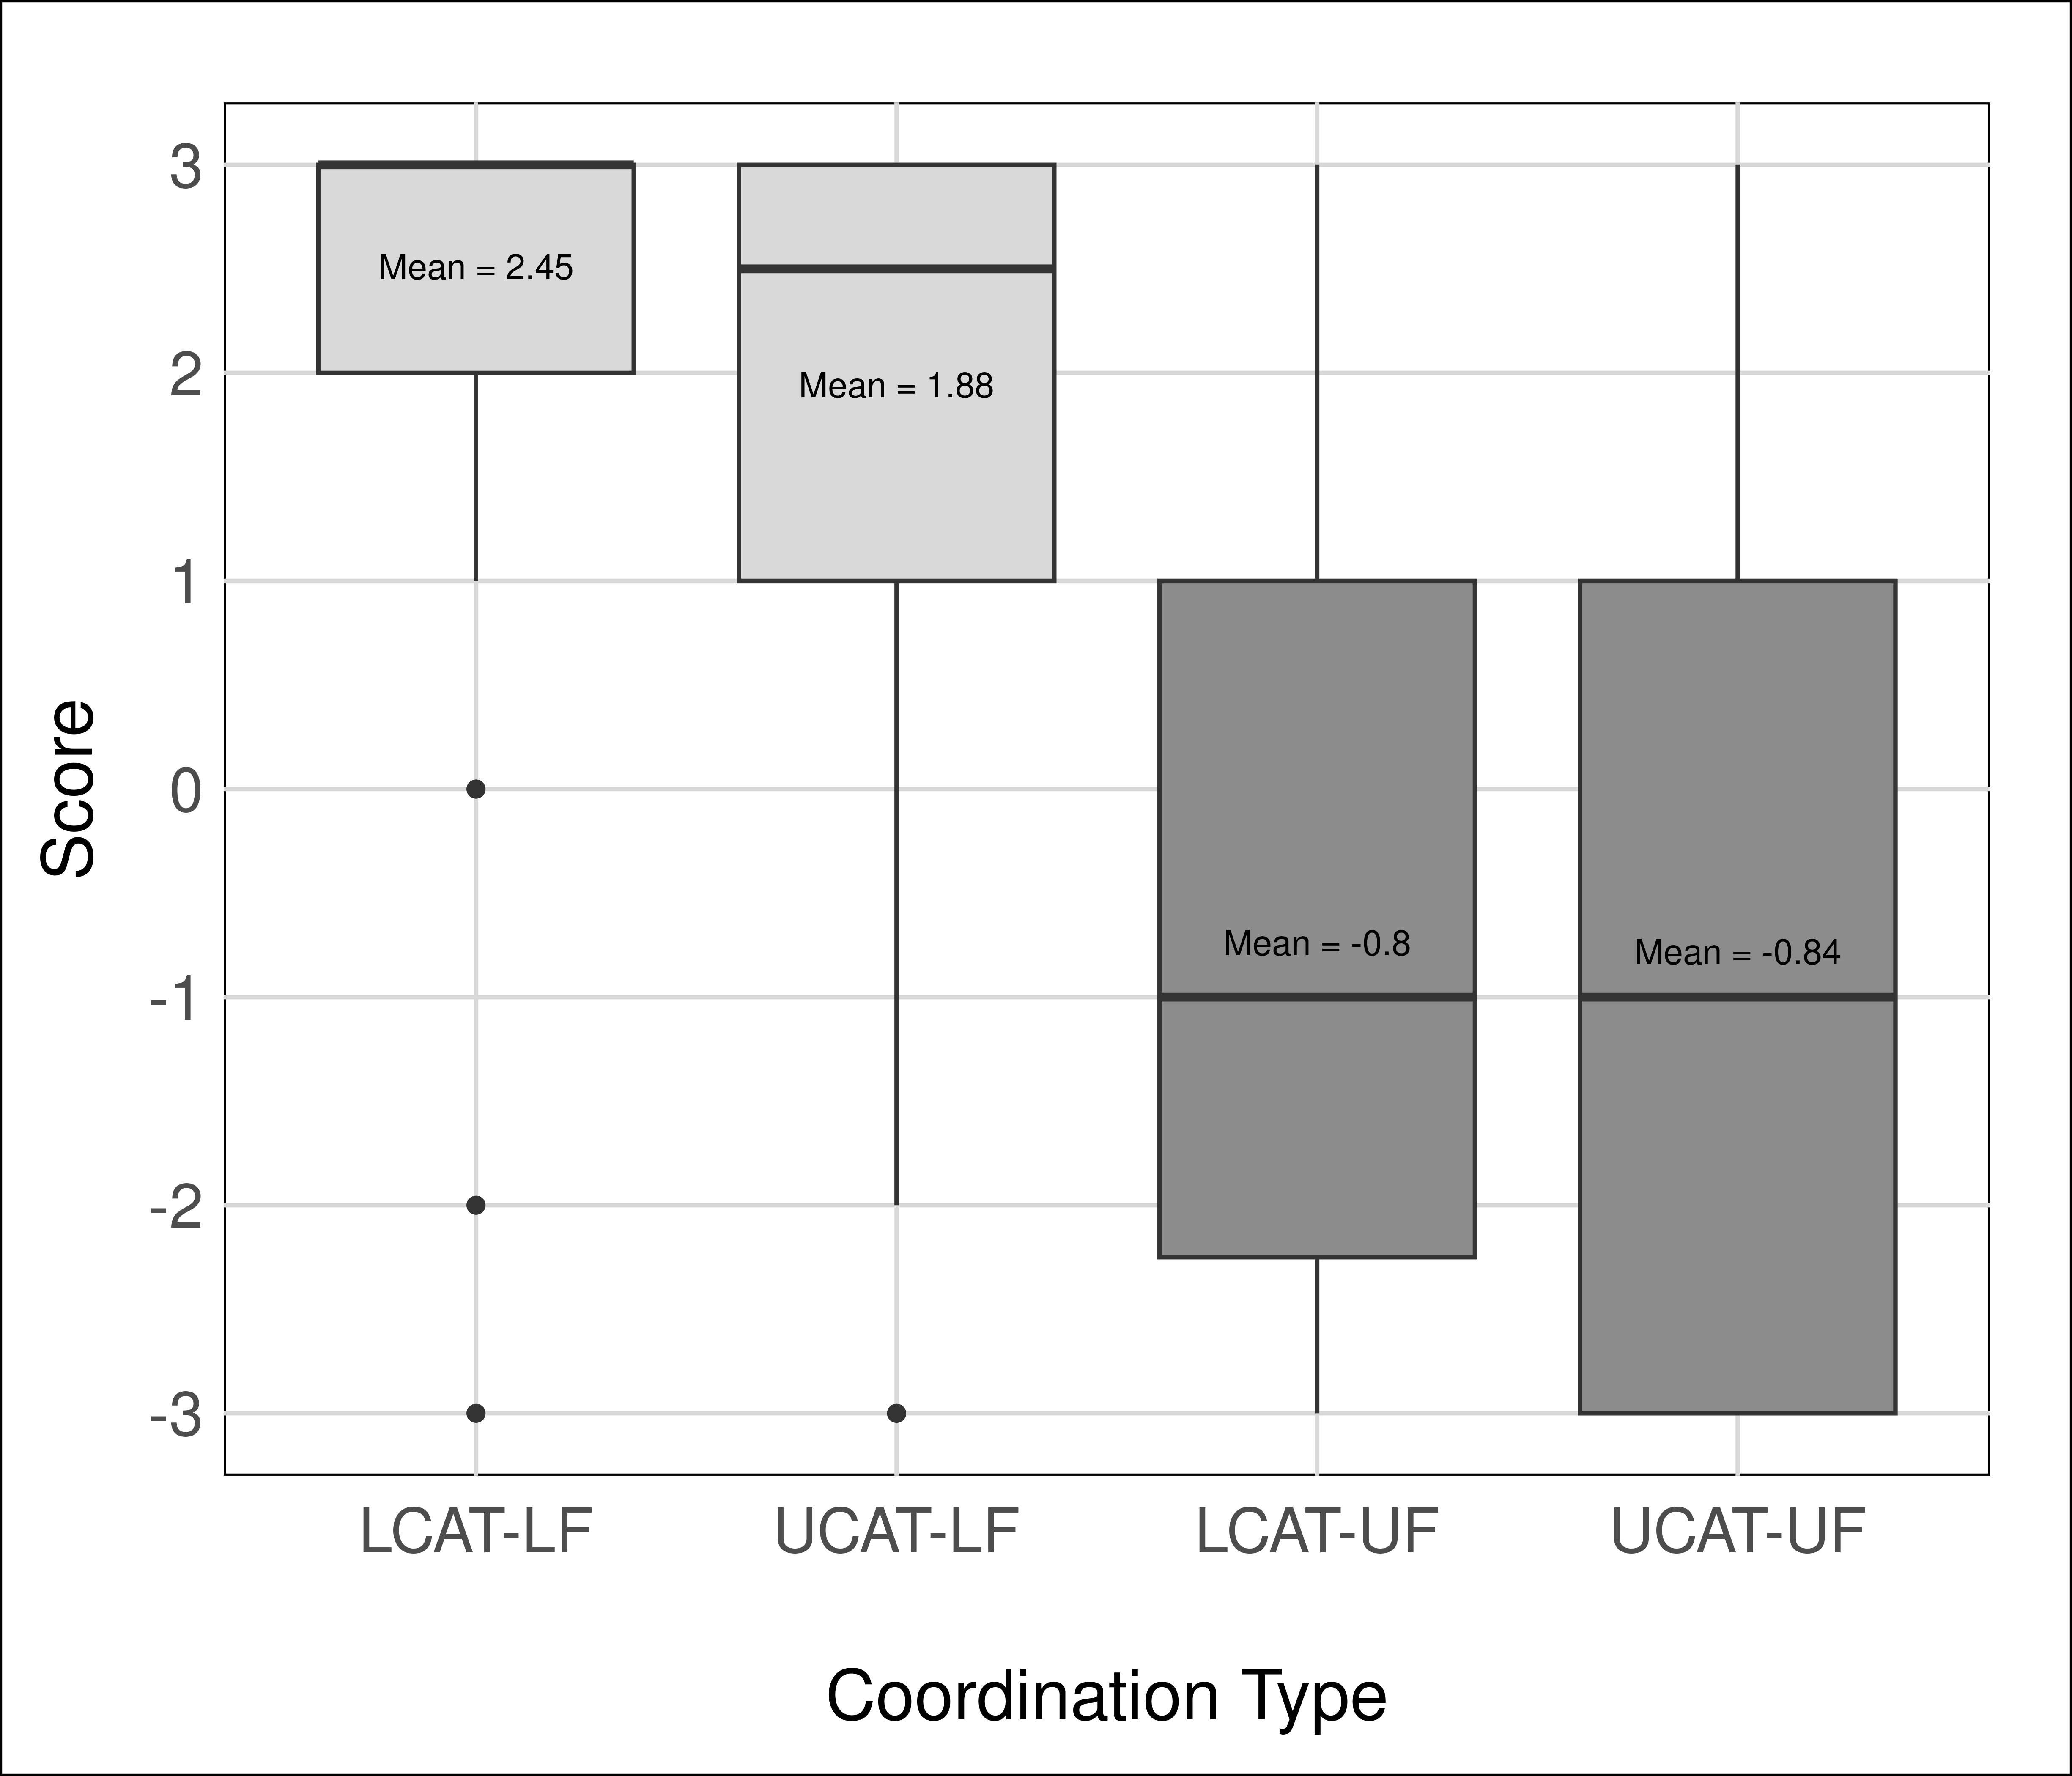
\includegraphics[width=0.88\linewidth]{images/updated_experiment/catboxplot.png}
	\caption{Boxplot for unlike category coordination experiment}
	\label{fig:catboxplot}
\end{figure}

\subsubsection{Inferential statistics}

Before fitting the linear mixed-effects models, several relevant comparisons between different pairs of conditions were carried out. A Wilcoxon signed-rank test was conducted to compare the scores for the LCAT-LF and UCAT-LF conditions. The test revealed a significant difference between the two conditions, with a test statistic (\textit{V}) of 2563 (\textit{p} < 0.001). This finding is in conflict with the part of the hypothesis that there should be no significant difference in acceptability so long as the conjuncts match in their functions. However, the same test demonstrated that UCAT-LF was also significantly different from both LCAT-UF (\textit{V} = 7735, \textit{p} < 0.001) and UCAT-UF (\textit{V} = 7394, \textit{p} < 0.001). 

Three distinct linear models were fitted to unlike category coordination data. In the first model, the distinct coordination configurations (i.e., LCAT-LF, UCAT-LF, LCAT-UF, UCAT-UF) were encoded as the levels of one independent variable called ``conditions.'' While this independent variable was specified as the fixed effect, IDs of the participants and token set indices were encoded as random effects. The exact R code used to fit the model can be seen in Figure \ref{fig:R_catmodelbasic}. Since the default optimiser of the `lmer()' function, the ``nloptwrap'' algorithm, failed to produce a fully convergent model, the ``bobyqa'' algorithm was used.

\begin{figure}[!h]
	\lstset{
		language=R,
		escapechar=@,
		basicstyle=\small\ttfamily,
		columns=fullflexible,
		keepspaces=true,
		keywordstyle=\color{black}\bfseries
	}
	\begin{lstlisting}
		control <- lmerControl(optimizer = "bobyqa")
		
		model_cat_1factor <- lmer(rating ~ condition +
		(1 + condition|participant_ID) +
		(1 + condition|tokenset),
		data = lm_cat_1factor,
		control = control)\end{lstlisting}
	\caption{R code for Model I of unlike category coordination experiment data}
	\label{fig:R_catmodelbasic}
\end{figure}


The relevant specifications of the first model (including some random effect statistics) are summarized in Figure \ref{tab:lmbasic}. 


\begin{table}[!h]
	\centering
	\begin{tabular}{llrr}
		\hline
		\hline
		\multicolumn{1}{c}{\textbf{}}        & \multicolumn{3}{c}{\textbf{acceptability}}                                            \\
		\multicolumn{1}{c}{\textit{Predictors}}       & \multicolumn{1}{c}{\textit{Estimates}} & \multicolumn{1}{c}{\textit{CI}} & \multicolumn{1}{c}{\textit{p}} \\ \hline
		(Intercept)                          & \multicolumn{1}{r}{2.45}      & 2.20 - 2.71            & \textbf{\textless{} 0.001}    \\
		condition {[}UCAT-LF{]}              & \multicolumn{1}{r}{--0.58}   &--1.04 - --0.13          & \textbf{0.012}                 \\
		condition {[}LCAT-UF{]}              & \multicolumn{1}{r}{--3.25}     & --3.75 - --2.75          & \textbf{\textless{} 0.001}    \\
		condition {[}UCAT-UF{]}              & \multicolumn{1}{r}{--3.29}     & --3.82 - --2.76          & \textbf{\textless{} 0.001}     \\
		\multicolumn{4}{l}{\textbf{Random Effects}}                                                                                    \\
		$\sigma$2                                   & \multicolumn{3}{l}{1.59}                                                       \\
		$\tau$00 participant\_ID                  & \multicolumn{3}{l}{0.04}                                                       \\
		$\tau$00 token\_set                       & \multicolumn{3}{l}{0.06}                                                       \\
		N participant\_ID                        & \multicolumn{3}{l}{48}                                                         \\ 
		N token\_set                         & \multicolumn{3}{l}{12}                                                         \\ \hline
		Observations                         & \multicolumn{3}{l}{576}                                                        \\
		Marginal R$^{2}$ / Conditional R$^{2}$        & \multicolumn{3}{l}{0.587 / NA}     \\    
		\hline \hline                                       
	\end{tabular}
	\caption{One independent variable model specifications}
	\label{tab:lmbasic}
\end{table}

In the context of a linear mixed effects model, the fixed effects refer to the parameters that are estimated to have a consistent effect on the outcome variable across all levels of the random effects. The respective coefficients of each level of the fixed effect are interpreted as follows:

\begin{itemize}
	\item \textbf{LCAT-LF}: The intercept coefficient of the model, which is 2.45 (\textit{SE} = 0.13, 95\% \textit{CI} [2.20, 2.71], \textit{p} < 0.001), represents the average rating for the LCAT-LF condition. This means that, on average, participants rated the LCAT-LF stimuli 2.45 on the scale. 
	
	\item \textbf{UCAT-LF}: The coefficient for the UCAT-LF condition is $-$0.58 (\textit{SE} = 0.17, 95\% \textit{CI} [--1.04, --0.13], \textit{p} = 0.012), indicating that participants rated the UCAT-LF stimuli slightly lower by 0.58 points, on average, compared to the LCAT-LF stimuli.
	
	\item \textbf{LCAT-UF}: The coefficient for the LCAT-UF condition is $-$3.25 (\textit{SE} = 0.25, 95\% \textit{CI} [--3.75, --2.75], \textit{p} < 0.001), which represents the difference in average scores between LCAT-UF and LCAT-LF when all other predictors are controlled for. The negative coefficient suggests that participants rated the LCAT-UF stimuli 3.25 points lower than the LCAT-LF stimuli, on average. 
	
	
	\item \textbf{UCAT-UF}: Finally, the coefficient for the UCAT-UF condition is $-$3.29 (\textit{SE} = 0.25, 95\% \textit{CI} [--3.82, --2.76], \textit{p} < 0.001), indicating that participants rated the UCAT-UF stimuli 3.29 points lower than the LCAT-LF stimuli, on average. 
\end{itemize}

Table \ref{tab:comparisons} below provides pairwise comparisons of conditions in the first model. Each row represents a specific comparison between two conditions. The ``Estimate'' column displays the estimated difference between the conditions. For example, in the LCAT-LF $\sim$ LCAT-UF comparison, the estimate of 3.2517 suggests that, on average, LCAT-LF condition is estimated to receive a higher score than the LCAT-UF condition. The ``SE'' column shows the standard error of the estimate while ``t-ratio'' column displays the calculated t-ratio for the comparison. The ``p-value'' column indicates the probability of obtaining the observed t-ratio or a more extreme value if the null hypothesis (no difference between the conditions) is true.

From the table, we can observe that the LCAT-LF $\sim$ LCAT-UF and LCAT-LF $\sim$ UCAT-UF comparisons have significant differences, as evinced by the very small p-values (both <0.0001). However, the LCAT-LF $\sim$ UCAT-LF comparison does not attain statistical significance (\textit{p} = 0.1114), suggesting that the difference between these conditions is not statistically significant. Similarly, the LCAT-UF $\sim$ UCAT-UF comparison shows that their negative impact on scores is virtually the same (\textit{p} = 0.9983). Moreover, the LCAT-UF $\sim$ UCAT-LF and UCAT-LF $\sim$ UCAT-UF comparisons both demonstrate significant differences, with p-values less than 0.0001.


\begin{table}[!ht]
	\centering
	\begin{tabular}{lrrrr}
		\textbf{Comparison} & \textbf{Estimate} & \textbf{SE} & \textbf{t-ratio} & \textbf{p-value} \\
		\hline \hline
		LCAT-LF $\sim$ UCAT-LF & 0.5810 & 0.232 & 2.508 & 0.1114 \\
		LCAT-LF $\sim$ LCAT-UF & 3.2517 & 0.256 & 12.682 & <0.0001 \\
		LCAT-LF $\sim$ UCAT-UF & 3.2941 & 0.270 & 12.186 & <0.0001 \\
		UCAT-LF $\sim$ UCAT-UF & 2.7132 & 0.372 & 7.298 & <0.0001 \\
		LCAT-UF $\sim$ UCAT-LF & $-$2.6708 & 0.299 & $-$8.934 & <0.0001 \\
		LCAT-UF $\sim$ UCAT-UF & 0.0424 & 0.258 & 0.164 & 0.9983 \\
		\hline
		\hline
	\end{tabular}
	\caption{Pairwise comparisons of conditions in Model I}
	\label{tab:comparisons}
\end{table}


The second model had two independent variables as fixed effects. These were the binary categorical variables of ``function'' and ``category'' where 1 indicated that conjuncts matched in their grammatical functions or categories, respectively. This model makes it possible to better isolate and estimate the individual impacts of functional and categorical matching between the conjuncts on the acceptability scores of the participants. While Figure \ref{fig:R_catmodel} shows the exact R code to fit the model, Figure \ref{fig:lmcat} lists the exact specifications of the second model. As this model could reach full convergence with the default optimizer algorithm, no alterations were introduced.

\begin{figure}[!h]
	\lstset{
		language=R,
		escapechar=@,
		basicstyle=\small\ttfamily,
		columns=fullflexible,
		keepspaces=true
	}
	\begin{lstlisting}
		model_cat <- lmer(rating ~ 
		function_match + category_match +
		(function_match + category_match | participant_ID) +
		(function_match + category_match | tokenset),
		data = lm_cat)\end{lstlisting}
	\caption{R code for Model II of unlike category coordination experiment data}
	\label{fig:R_catmodel}
\end{figure}

\begin{table}[!h]
	\centering
	\begin{tabular}{llrr}
		& \multicolumn{3}{c}{\textbf{acceptability}}                   \\
		\textit{Predictors} & \textit{Estimates}        & \multicolumn{1}{l}{\textit{CI}} & \multicolumn{1}{l}{\textit{p}} \\ \hline
		(Intercept)                  & \multicolumn{1}{r}{2.32}  & {2.00} - {2.65}   & \textless{}0.001 \\
		function mismatch   & \multicolumn{1}{r}{--2.99} & {--3.46} - {--2.51}                   & \textless{}0.001               \\
		category mismatch            & \multicolumn{1}{r}{--0.31} & --0.59 - --0.03 & 0.029            \\
		\multicolumn{4}{l}{\textbf{Random Effects}}                                                 \\
		$\sigma^{2}$                           & \multicolumn{3}{l}{1.79}                                     \\
		$\tau$00 participant\_ID          & \multicolumn{3}{l}{0.16}                                     \\
		$\tau$00 token\_set               & \multicolumn{3}{l}{0.18}                                     \\
		N participant\_ID                        & \multicolumn{3}{l}{48}                                                         \\ 
		N token\_set                 & \multicolumn{3}{l}{12}                                       \\ \hline
		Observations                 & \multicolumn{3}{l}{576}                                      \\
		Marginal R$^{2}$ / Conditional R$^{2}$ & \multicolumn{3}{l}{0.558 / NA}  \\ \hline \hline                            
	\end{tabular}
	\caption{Two independent variables model specifications}
	\label{fig:lmcat}
\end{table}


The intercept of the second model, which represents the average score when both functions and categories of the conjuncts match, was found to be 2.32 (\textit{SE} = 0.16, 95\% \textit{CI} [2.00, 2.65], \textit{p} < 0.001). The estimated coefficient for function mismatch was $-$2.99 (\textit{SE} = 0.23, 95\% \textit{CI} [$-$3.46, $-$2.51], \textit{p} < 0.001), indicating that when the functions of the conjuncts do not match, the average rating is expected to decrease by 2.99. The coefficient for category mismatch was $-$0.31 (\textit{SE} = 0.14, 95\% \textit{CI} [$-$0.59, $-$0.03], \textit{p} = 0.029), suggesting that the average rating is expected to decrease by 0.31 when the conjuncts have different syntactic categories.

The results of this model suggest that both function mismatch and category mismatch have a significant impact on the acceptability ratings. When the functions of the conjuncts do not match, however, the acceptability scores dramatically decrease, while a mismatch in syntactic categories leads to only a slight decrease in scores.

Note that the intercept of the second model refers to the score of the condition LCAT-LF. It is, however, different from the intercept of the first model, which corresponds to the same variable. This stems from the fact that the second model does not take into account the interaction between the two fixed effects. For this reason, a third model was also fit to the data to account for the interaction between the fixed effects of function mismatch and category mismatch as well. The Figure \ref{fig:R_catmodel2} demonstrates the exact R code used to fit the model. The Table \ref{tab:catmodel3}, on the other hand, provides the estimates, confidence intervals, and p-values for each predictor in this model. 


\begin{figure}[!h]
	\lstset{
		language=R,
		escapechar=@,
		basicstyle=\small\ttfamily,
		columns=fullflexible,
		keepspaces=true
	}
	\begin{lstlisting}
		model_cat_interaction <- lmer(rating ~ 
		function_match * category_match +
		(function_match + category_match | participant_ID) +
		(function_match + category_match | tokenset),
		data = lm_cat)\end{lstlisting}
	\caption{R code for Model III of unlike category coordination experiment data}
	\label{fig:R_catmodel2}
\end{figure}


\begin{table}[!h]
	\centering
	\begin{tabular}{llrr}
		\hline \hline
		\multicolumn{1}{c}{\textbf{}}         & \multicolumn{3}{c}{\textbf{acceptability}}                          \\
		\multicolumn{1}{c}{\textit{Predictors}} & \multicolumn{1}{c}{\textit{Estimates}} & \multicolumn{1}{c}{\textit{CI}} & \multicolumn{1}{c}{p} \\ \hline
		(Intercept)                           & \multicolumn{1}{r}{2.45}  & 2.11 – 2.80   & \textless{}0.001 \\
		function mismatch                     & \multicolumn{1}{r}{-3.26} & -3.78 – -2.73 & \textless{}0.001 \\
		category mismatch                     & \multicolumn{1}{r}{-0.58} & -0.94 – -0.22 & 0.002            \\
		function mismatch × category mismatch & \multicolumn{1}{r}{0.54}  & 0.10 – 0.98   & 0.015            \\
		\multicolumn{4}{l}{\textbf{Random Effects}}                                                          \\
		$\sigma$2                                    & \multicolumn{3}{l}{1.77}                                     \\
		$\tau$00 participant\_ID                   & \multicolumn{3}{l}{0.16}                                     \\
		$\tau$00 token\_set                        & \multicolumn{3}{l}{0.18}                                     \\
		N participant\_ID                        & \multicolumn{3}{l}{48}                                                         \\
		N token\_set                          & \multicolumn{3}{l}{12}                                       \\ \hline
		Observations                          & \multicolumn{3}{l}{576}                                      \\
		Marginal R2 / Conditional R2          & \multicolumn{3}{l}{0.563 / NA} \\ \hline \hline                              
	\end{tabular}
	\caption{Two independent variables + interaction model specifications}
	\label{tab:catmodel3}
\end{table}
The intercept of the third model (see Table \ref{tab:catmodel3}) indicates that the expected acceptability rating is 2.45 when conjuncts match both in their functions and categories (\textit{SE} = 0.17, 95\% \textit{CI} [2.11, 2.80], \textit{p} < 0.001). The estimate for the function mismatch variable is $-$3.26 (\textit{SE} = 0.26, 95\% \textit{CI} [$-$3.78, $-$2.73], \textit{p} < 0.001), indicating that a mismatch of functions is associated with an (average) decrease of 3.26 in the acceptability rating when other predictors are held constant. The estimate for the category mismatch is $-$0.58 (\textit{SE} = 0.18, 95\% \textit{CI} [$-$0.94, $-$0.22], \textit{p} = 0.002). That is, mismatching categories of conjuncts is associated with a decrease of 0.58 in the acceptability rating. 

The interaction predictor, function mismatch $\times$ category mismatch, has an estimate of 0.54 (\textit{SE} = 0.22, 95\% \textit{CI} [0.10, 0.98], \textit{p} = 0.015). This means that, on average, when both the functions and the categories of conjuncts mismatch, their cumulative negative effect on the acceptability rating becomes less severe. To calculate the combined effect, we would sum the estimates of the individual main effects (-3.26 for function mismatch and -0.58 for category mismatch) along with the estimate for the interaction term, which is 0.54.


\subsubsection{Discussion}

The results obtained from the three models demonstrate that a functional match between the conjuncts is a crucial factor in the acceptability rate of a coordinate structure. In the first model, the conditions where the conjuncts have different functions (i.e., LCAT-UF and UCAT-UF) have large negative impacts on the acceptability ratings. The predictors of the second model indicates that the functional match between conjuncts has the biggest impact on the acceptability ratings with a coefficient estimate of $-$2.99. In the third model, the negative impact of mismatching functions becomes more pronounced at an estimated coefficient of $-$3.26 when the model accounted for the interaction effects between the predictors.

With the exception of the pairwise comparisons in Model I (see Table \ref{tab:comparisons}), all the analyses show that there is a significant difference between LCAT-LF and UCAT-LF in their acceptability rates. Thus, a categorical incongruity between the conjuncts seems to have a statistically significant impact on the acceptability rate. This impact, however, is not substantial as can be seen from the relevant coefficients of categorical predictors in the models. Furthermore, UCAT-LF is by no means an utterly unacceptable construction as it received a mean score of 1.88 and a median of 2.5 compared to the negative mean scores of LCAT-UF and UCAT-UF conditions. 

Based on the results, two distinct conclusions can be drawn. First, we can challenge the original hypothesis and propose a more flexible version of it, implying that the mismatch between syntactic categories or cases could potentially exert a significant influence on acceptability. Alternatively, we can seek to retain the original hypothesis by considering the impact of frequency factors on acceptability. Within the context of the present findings, LCAT-LF, which is the standard type of coordination in Turkish, is undeniably much more frequent in Turkish corpora than UCAT-LF. In experimental syntax literature, there is a substantial body of evidence indicating that structures with low frequencies tend to receive lower acceptability ratings when compared to high-frequency structures, assuming both structures are grammatical \citep{Bresnan2007, Divjak2016, Francis2021}. Therefore, a minor disparity in favor of the LCAT-LF condition is expected.

As a result, the present thesis leans towards the latter conclusion, thereby upholding the original hypothesis. This stance essentially asserts that the slight variation in acceptability ratings between the conditions could be attributed to the frequency difference between the LCAT-LF and UCAT-LF conditions.

\subsection{Coordination of unlike cases}
\subsubsection{Descriptive statistics}

As demonstrated in Table \ref{tab:unlikecase_descriptive}, the mean rating for LCASE-LF coordination type is 2.32, with a standard deviation of 1.38. The median rating is 3, indicating a generally positive evaluation of this coordination type, which is not surprising as this is the standard type of coordination in Turkish. On the other hand, the mean rating for UCASE-LF coordination type is 1.58, with a higher standard deviation of 1.71. The median rating is 2.00, suggesting a positive evaluation of this coordination type, but with more variability than LCASE-LF. Finally, the mean rating for UCASE-UF coordination type is negative at $-$0.37, with the highest standard deviation of 2.04. The median rating is $-$1.00, indicating an overall negative evaluation of this coordination type. 

\begin{table}[ht]
	\centering
	\begin{tabular}{lrrrrrr}
		\textbf{Coordination type} & \textbf{N} & \textbf{Mean} & \textbf{SD} & \textbf{Min} & \textbf{Max} & \textbf{Median}  \\ 
		\hline \hline
		LCASE-LF & 144 &2.32 & 1.38 &  $-$3 &   3 & 3.00  \\ 
		UCASE-LF & 144 &1.58 & 1.71 &  $-$3 &   3 & 2.00  \\ 
		UCASE-UF & 144 &$-$0.37 & 2.04 &  $-$3 &   3 & $-$1.00  \\ 
		\hline \hline
	\end{tabular}
	\caption{Descriptive statistics of unlike case coordination experiment}
	\label{tab:unlikecase_descriptive} 
\end{table}

Participants strongly agree that LCASE-LF is highly acceptable, as can be seen in Figure \ref{fig:lmcase}. The scores of UCASE-LF, however, show more variability as the IQR box is relatively more spread out between the scores of 1 and 3. UCASE-LF, however, still seems to be an acceptable type as the distribution is again considerably left-skewed towards the positive end of the scale. UCASE-UF, on the other hand, seems to be slightly right-skewed towards the negative end of the scale. The variability of UCASE-UF scores, however, is quite high as IQR box is extended between the scores of $-$2 and 1.


\begin{figure}[!h]
	\centering
	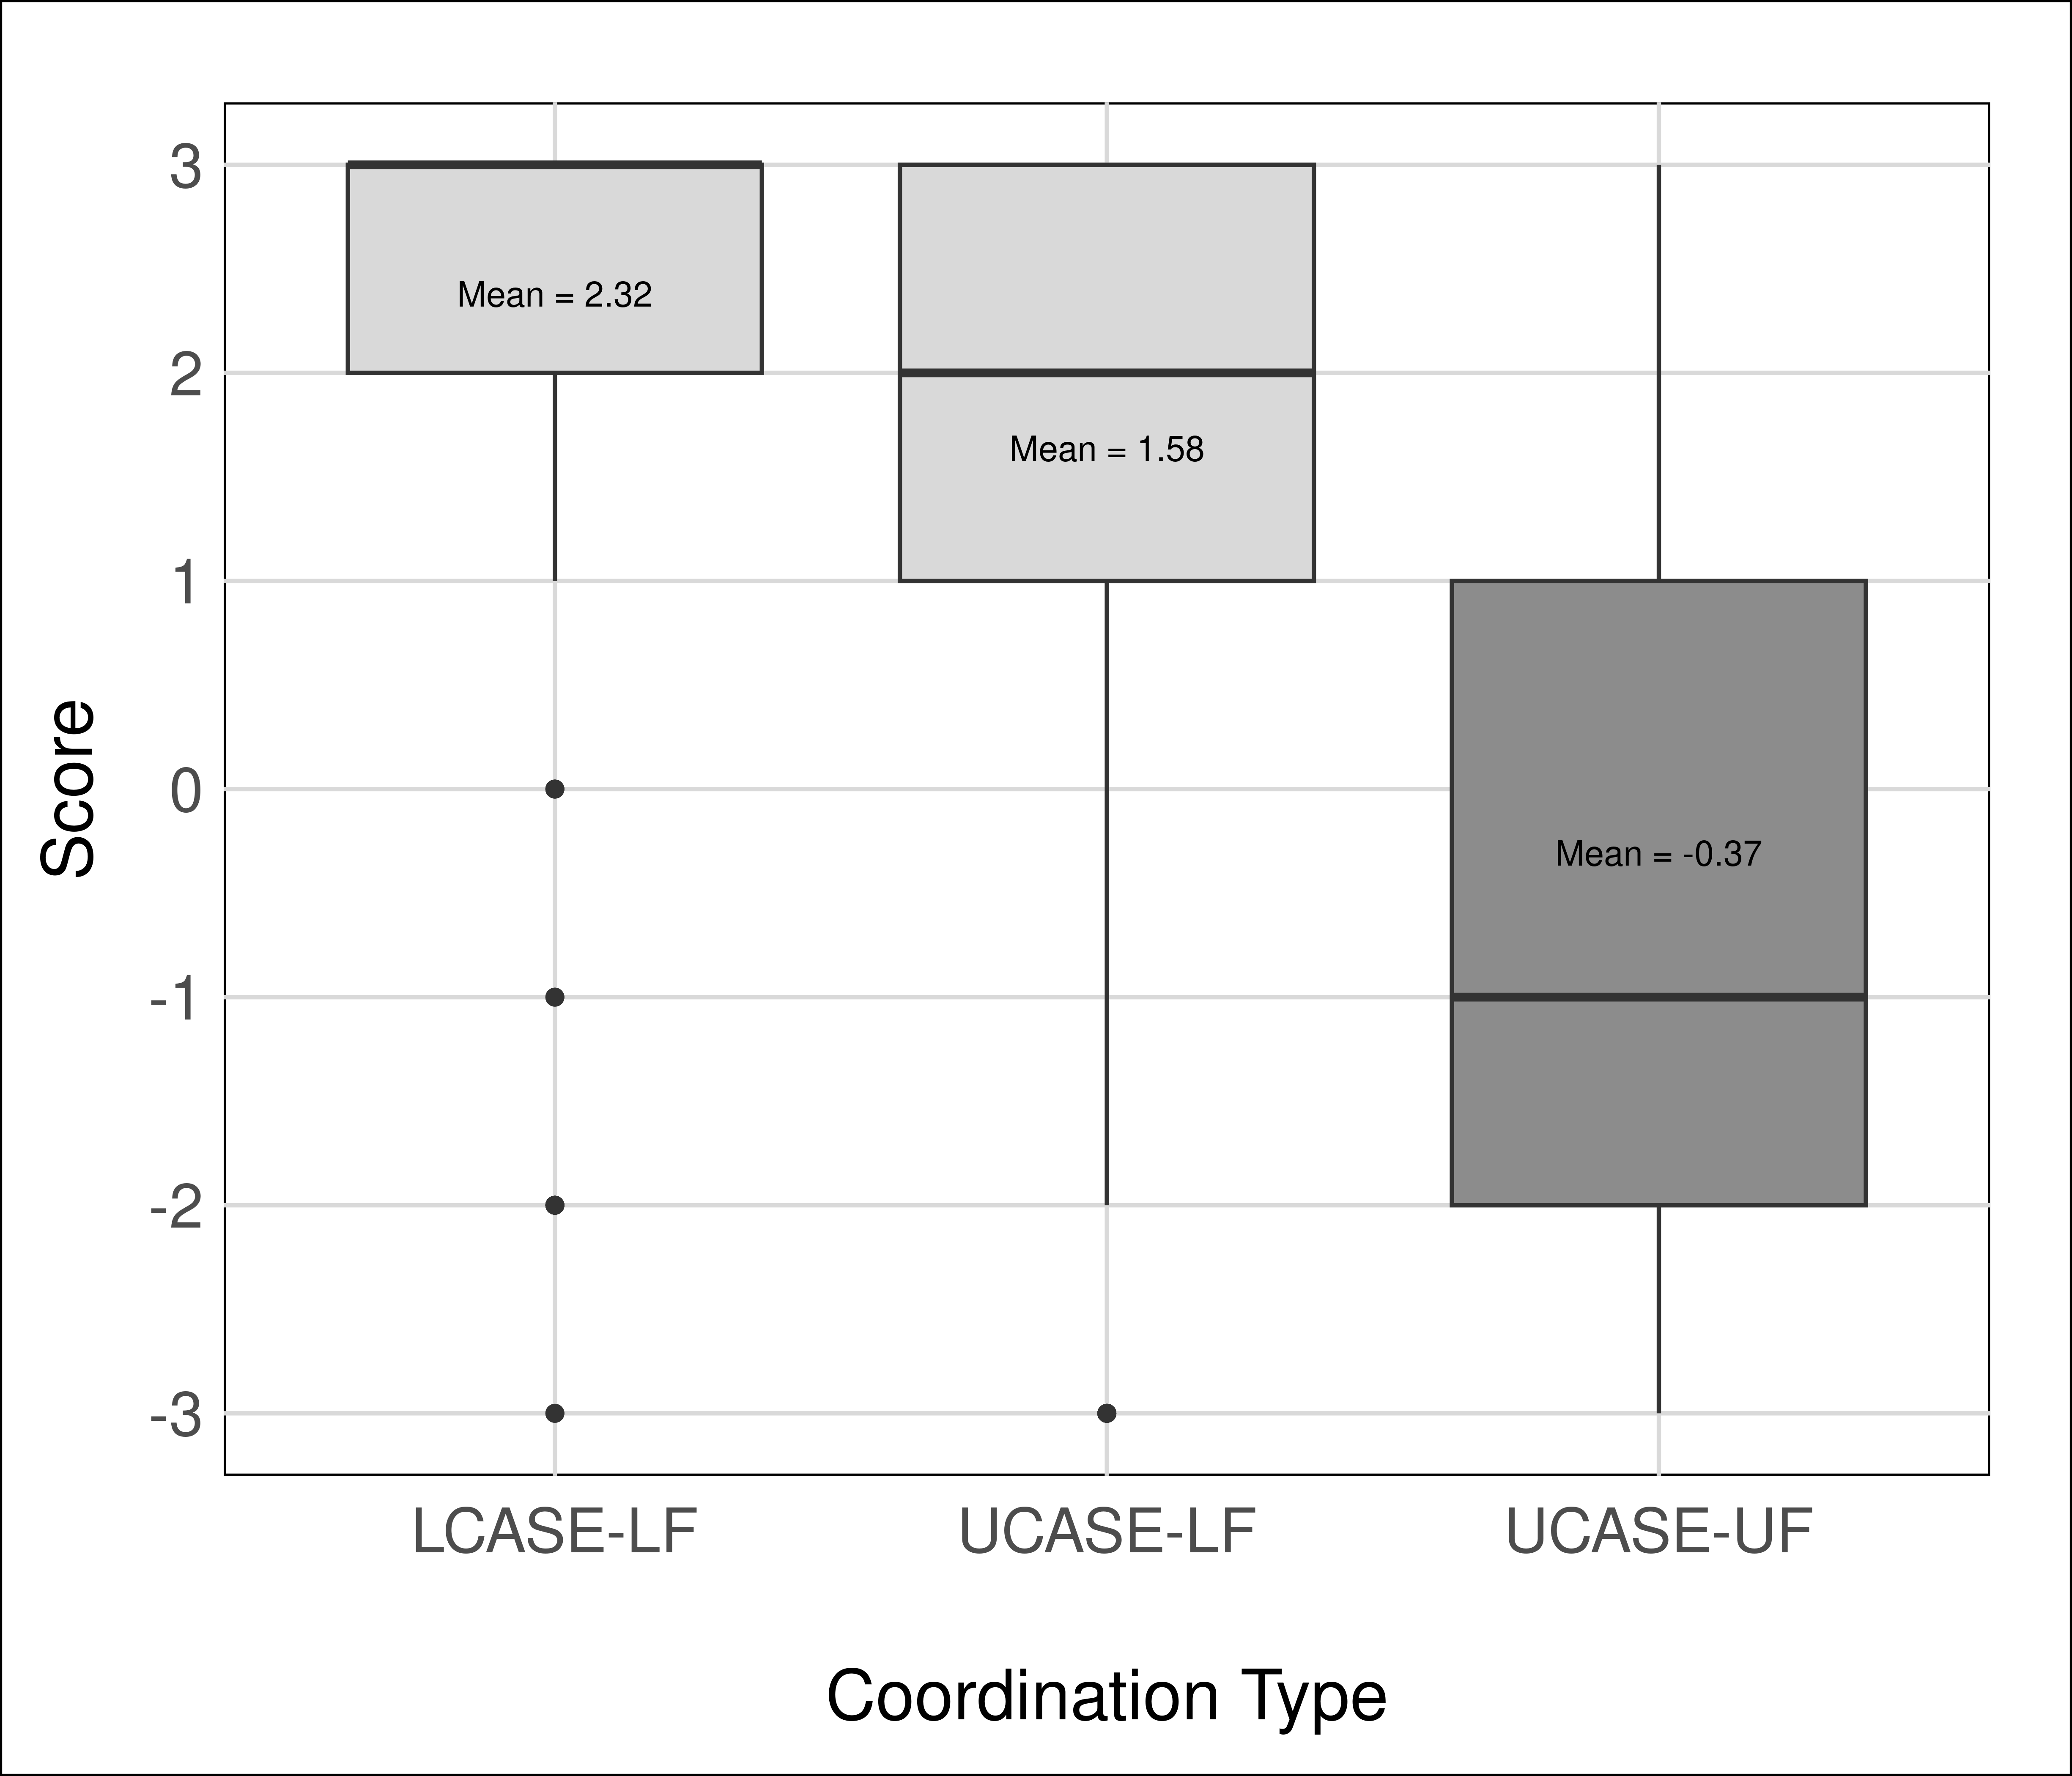
\includegraphics[width=0.88\linewidth]{images/updated_experiment/caseboxplot.png}
	\caption{Boxplot for unlike case coordination experiment}
	\label{fig:lmcase}
\end{figure}


\subsubsection{Inferential Statistics}

Similar to the analyses of unlike category coordination experiment, in addition to fitting a linear mixed-effects model, several Wilcoxon signed-rank tests were conducted to compare relevant pairs of conditions. The difference between LCASE-LF and UCASE-LF was significant (\textit{V} = 2655, \textit{p} < .001), confirming that mismatching cases of conjuncts had a significant negative impact on acceptability. However, the difference between UCASE-LF and UCASE-UF was also significant (\textit{V} = 5859, \textit{p} < .001), suggesting functional incongruity between the conjuncts also had a considerable negative impact on acceptability.

As opposed to the unlike category coordination experiment, only one linear mixed-effects model was fitted to the data as unlike case coordination experiment did not have a proper 2$\times$2 factorial design (see \S \ref{sec:experimentaldesign}). This model is practically the same as the first model used to analyze the unlike category coordination experiment.

This model had one independent variable called ``condition'' encoded as the fixed effect. The distinct types of coordination (i.e., LCASE-LF, UCASE-LF, UCASE-UF) were analyzed as the levels of this variable. The random effects were the same as the previous models: IDs of the participants and the token set indices. Since this model also did not fully converge with the default optimizer algorithm, ``bobyqa'' algorithm had to be manually introduced. The exact code used to fit the model can be seen in Figure \ref{fig:R_casemodel}. The specifications of the fitted model are summarized in Table \ref{tab:lmcase_model}. 

\begin{figure}[!h]
	\lstset{
		language=R,
		escapechar=@,
		basicstyle=\small\ttfamily,
		columns=fullflexible,
		keepspaces=true
	}
	\begin{lstlisting}
		control <- lmerControl(optimizer = "bobyqa")
		
		model_case = lmer(rating ~ condition + 
		(1 + condition|participant_ID) +
		(1 + condition|tokenset), 
		data = lm_case,
		control = control)\end{lstlisting}
	\caption{R code for the model of unlike case coordination experiment data}
	\label{fig:R_casemodel}
\end{figure}


\begin{table}[!h]
	\centering
	\begin{tabular}{llrr}
		\hline \hline
		\multicolumn{1}{c}{\textbf{}} & \multicolumn{3}{c}{\textbf{acceptability}}                          \\
		\multicolumn{1}{c}{\textit{Predictors}} & \multicolumn{1}{c}{\textit{Estimates}} & \multicolumn{1}{c}{\textit{CI}} & \multicolumn{1}{c}{\textit{p}} \\ \hline
		(Intercept)                   & \multicolumn{1}{r}{2.32}  &2.02 -- 2.62   & \textless{}0.001 \\
		condition {[}UCASE-LF{]}        & \multicolumn{1}{r}{-0.75} &-1.15 -- -0.34 & \textless{}0.001 \\
		condition {[}UCASE-UF{]}        & \multicolumn{1}{r}{-2.70} & -3.31 – -2.09 & \textless{}0.001 \\
		\multicolumn{4}{l}{\textbf{Random Effects}}                                                  \\
		$\sigma$2                            & \multicolumn{3}{l}{1.93}                                     \\
		$\tau$00 participant\_ID           & \multicolumn{3}{l}{0.22}                                     \\
		$\tau$00 token\_set                & \multicolumn{3}{l}{0.06}                                     \\
		N token\_set                  & \multicolumn{3}{l}{12}                                       \\ \hline
		Observations                  & \multicolumn{3}{l}{432}                                      \\
		Marginal R2 / Conditional R2  & \multicolumn{3}{l}{0.300 / 0.554}  \\ \hline \hline                      
	\end{tabular}
	\caption{One independent variable case model specficiations}
	\label{tab:lmcase_model}
\end{table}


As revealed by the model, participant scores were significantly affected by the experimental conditions UCASE-LF and UCASE-UF. The intercept, representing the expected score for LCASE-LF, was estimated to be 2.32 (\textit{SE} = 0.15, 95\% \textit{CI} [2.02, 2.62], \textit{p} < 0.001). The scores given to UCASE-LF stimuli were 0.75 points lower (\textit{SE} = 0.20, 95\% \textit{CI} [$-$1.15, $-$0.34], \textit{p} < 0.001) than LCASE-LF condition, on average. UCASE-UF stimuli received 2.70 points lower scores (\textit{SE} = 0.31, 95\% \textit{CI} [$-$3.31, $-$2.09], \textit{p} < 0.001) than LCASE-LF condition, on average.

These coefficients indicate that both experimental conditions have significant negative effects on participant scores, compared to LCASE-LF, which is the standard type of coordination in Turkish. However, the negative effect is considerably larger for the UCASE-UF condition than for the UCASE-LF condition.

\subsubsection{Discussion}

The combined results from the linear mixed-effects model and Wilcoxon signed-rank test comparisons draw a picture similar to the unlike category coordination experiment. Functional matching is indeed the most important factor when it comes to the acceptability of Turkish coordinate structures. Mismatching case configuration alone was not able to engender a highly negative response from the participants despite being a significant and slightly negative predictor of acceptability ratings. Furthermore, the UCASE-UF condition cannot also be considered as an outright unacceptable condition, as the mean score of UCASE-UF is still significantly higher than the mean score of ungrammatical fillers.

Once again, these findings lend support to the hypothesis that regards functional matching between the conjuncts as the essential factor behind the acceptability of Turkish coordinate structures.

\section{Conclusion} \label{sec:conclusionexp}

This chapter discussed the methodology and results of the formal acceptability judgment experiment conducted within the context of the present thesis. The experiment provided data that is valuable not only within the scope of the present thesis but also in terms of the general theoretical research on coordination.

The results strongly support the claim that the functional congruence between the conjuncts is the main driving factor behind the acceptability of Turkish coordinate structures. However, the claim that functional congruence is the only significant factor behind acceptability could be problematic if one does not acknowledge the impact of frequency factors on acceptability ratings. Furthermore, both UCAT-LF and UCASE-LF received considerably positive ratings and should ultimately be considered as highly acceptable constructions.

The acceptability experiment further evaluated the acceptability rates of coordination configurations featuring mismatching functions, denoted by conditions ending with UF. The tested configurations also included different types of absolute unlike coordination that were not encountered within the corpus. The results of the experiment suggest that all such configurations have a significantly negative effect on acceptability. Notably, the rarity of these constructions in the corpus appropriately mirrors their ungrammatical status. Overall, the results of the acceptability experiment align with the results of the corpus investigation.

	\chapter{Formal analysis} \label{ch:formal_analysis}
	\section{Overview of the chapter}

This chapter presents a formal analysis of Turkish unlike coordination phenomena within the framework of Lexical-Functional Grammar (LFG). In \S\ref{sec:frameworksofsyntax}, the rationale for adopting this particular theoretical framework is justified. Next, in \S\ref{sec:lfg}, the fundamental properties of LFG are introduced, providing essential background information for the analysis. \S\ref{sec:lfganalysis} presents a detailed formal analysis of Turkish unlike coordination within the context of distinct syntactic configurations. Finally, \S\ref{sec:exampleanalysis} demonstrates how the analysis works within the context actual examples of unlike coordination.

\section{Frameworks of syntax}\label{sec:frameworksofsyntax} 

Modern approaches to natural language syntax can be broadly classified into two overarching frameworks \citep{pullumetal_2001}: \textit{generative-enumerative syntax} and \textit{model-theoretic syntax}. Although these two frameworks share the common goal of capturing the syntactic parameters of natural languages, they differ significantly in their approaches to achieving this objective.

\textit{Generative-enumerative syntax} (henceforth abbreviated as GES) has its origins in the syntactic component of mathematical logic and formal language theory, with foundational contributions made by \citet{Chomsky1959}. Within the GES framework, language is viewed as a (potentially infinite) collection of strings generated by a formal ``device.'' This formal device consists of a finite set of rewrite rules, often referred to as phrase-structure rules, and lexical items. Consequently, the responsibility of this device is to generate (and enumerate) all and only the grammatical strings of a given language. Accordingly, linguists working within the GES framework endeavor to formulate a precise set of rules for this device that can adequately account for grammatical strings while avoiding the generation of ungrammatical ones. Prominent theoretical approaches following GES include Minimalism \citep{Chomsky1993} and its precursor, Government and Binding Theory \citep{Chomsky1981}, as well as Tree-Adjoining Grammars \citep{Joshi1987} and various forms of categorial grammars.

In contrast to GES, \textit{model-theoretic syntax} (henceforth abbreviated MTS) primarily originates from the semantic domain of mathematical logic. Unlike GES, MTS does not rely on rewrite rules but rather employs a set of constraints to define syntax. These constraints do not aim to exhaustively enumerate all and only the grammatical strings of a given language. Instead, they collectively define syntax by specifying the necessary conditions for the desired syntactic structure of a valid natural language string. Consequently, a natural language string is deemed grammatical if it satisfies the constraints formulated by a linguist, while it is considered ungrammatical if it violates them. It is important to note that these constraints do not generate syntactically well-formed strings, neither conceptually nor formally. Rather, they model possible syntactic structures that can characterize a well-formed string.  Notable MTS-based approaches include Head-Driven Phrase Structure Grammar (HPSG; \citealp{pollardetal1994, muller:2021}) and Lexical-Functional Grammar (LFG; \citealp{kaplan&bresnan_1982, Dalrymple2019}).

MTS-based approaches offer several advantages over their GES-based counterparts both in formal and empirical domains (for an overview, see \citealp{pullumetal_2001, Sag2011}). One notable advantage of MTS-based approaches lies in their ability to account for gradience in ungrammaticality, a feature lacking in GES-based approaches. In GES-based approaches, grammars generate all and only the grammatical strings that form a set. Thus, a given sentence either belongs to this set (grammatical) or not (ungrammatical). However, this binary classification fails to capture the varying degrees to which a sentence violates syntactic rules. To exemplify this issue, consider the following sentences in (\ref{tonysoprano}). 

\pex[glspace=!1em,everygla={},everyglb={},aboveglbskip=-.15ex, interpartskip=5pt]
\label{tonysoprano}
\a \label{tonysopranoa}A wrong decision is better than indecision.
\a \label{tonysopranob}\ljudge{*} A wrong decision are better than indecision.
\a \label{tonysopranoc}\ljudge{**} Decision a better wrong is indecision than.
\xe

In a GES-based grammar of English, both (\ref{tonysopranob}) and (\ref{tonysopranoc}) would be classified as ungrammatical since they do not belong to the generated set of grammatical strings. While both sentences are indeed ungrammatical, the extent to which they violate the syntactic rules of English differs. Sentence (\ref{tonysopranob}) still retains some ability to express a proposition, albeit with a subject-verb agreement error. In contrast, sentence (\ref{tonysopranoc}) fails to convey any coherent meaning at all. However, within the GES framework, there is no inherent mechanism to account for gradience in ungrammaticality, as grammaticality is treated as a binary property tied to set membership.

On the other hand, an MTS-based grammar provides the necessary tools to model degrees of ungrammaticality. A given string does not need to violate all syntactic constraints simultaneously. For instance, sentence (\ref{tonysopranob}) violates only the constraint that governs the number and person agreement between subject and verb in English, while satisfying all other syntactic constraints. In contrast, sentence (\ref{tonysopranoc}) violates numerous constraints of English syntax. Consequently, an MTS-based grammar can effectively explain and measure the degrees of grammaticality by assessing the number of constraint violations, rather than relying solely on set membership.

Another advantage of MTS stems from its ability to effectively model the incremental processing of language, a crucial aspect of real-life language comprehension.  When individuals encounter a sentence, they begin constructing its meaning and syntactic structure as soon as they start perceiving the linguistic input, without waiting for the full utterance to conclude. This incremental processing involves constant revision and updating of the partial structure in their minds as new linguistic items unfold.\footnote{This phenomenon of incremental processing has been extensively supported by a wealth of psycholinguistic research. See \citet{Levelt1993}, \citet{Tanenhaus1995}, and \citet{VONDERMALSBURG2011}.} 

To effectively model this dynamic and incremental process, a formal mechanism is required to construct and evaluate partial structures. GES-based approaches, however, fall short in this regard since their rewrite rules solely enumerate complete expressions and exclude the fragments that constitute them. For instance, the string \textit{a wrong decision is} does not exist within the set of grammatical strings in GES-based grammars. Consequently, it is treated no differently than a randomly ordered sequence of symbols. 

In contrast, MTS-based approaches, such as HPSG and LFG, are equipped to handle partial structures. In these approaches, the string \textit{a wrong decision} is analyzable and already satisfies numerous constraints pertaining to the structure of English NPs and subject-verb agreement, among others. Moreover, lexical items in MTS-based approaches inherently carry diverse morphosyntactic information regardless of whether they are part of a larger syntactic construction. This means that even as isolated expressions, lexical items contribute to (partial) meaning and morphosyntactic structure. This feature-rich nature of lexical items enables MTS-based approaches to account for partial expressions giving rise to both meaning and morphosyntactic structure. Consequently, it can be claimed that MTS-based approaches enable linguists to more accurately model the intricacies of linguistic knowledge in humans.

Building upon the advantages offered by MTS foundations, this thesis proposes a formal analysis of Turkish coordination within an MTS-based framework, namely Lexical-Functional Grammar (LFG). While LFG also incorporates elements from GES, the analysis presented here integrates mechanisms proposed in previous works to align LFG more closely with the core principles of MTS. Thus, the analysis not only provides a formalized account of the empirical findings regarding Turkish coordination but also exemplifies a form of LFG that more closely adheres to the core principles of MTS.

	\section{Lexical-Functional Grammar} \label{sec:lfg}

\subsection{Overview of LFG architecture}

LFG emerged as a compelling alternative to the prevailing transformative framework in 1970s. It was proposed by Joan Bresnan, a linguist, and Ronald Kaplan, a psychologist. The motivation behind their proposal primarily arose from the transformative framework's shortcomings in terms of psychological plausibility and its limited ability to model crosslinguistic generalizations effectively \citep[pp.\ 1--2]{Dalrymple2019}. Unlike transformative frameworks, as well as other constraint-based frameworks, LFG posits a modular architecture of grammar, wherein distinct forms of linguistic knowledge are represented at different formal levels. Crucially, these levels are interconnected through well-defined mappings (\textit{projections}), enabling the exchange of information across levels.

In LFG, syntax is handled through two key levels: c-structure (constituent structure) and f-structure (functional structure). To elucidate these distinct structures, let us consider the sentence (\ref{tonylikes}) and its corresponding LFG analysis, as portrayed in Figure \ref{fig:tonylikes}.

\pex
\label{tonylikes}
Tony likes the book.
\xe

The syntax of the sentence is captured by two distinct data structures that are systematically connected. C-structure (depicted on the left) is a phrase-structure tree, generated using a specific type of phrase-structure rules encoded in the grammar. At the c-structure level, the information is primarily concerned with the linear order of words and the underlying constituent structure of the sentence. By contrast, the f-structure (presented on the right) represents more abstract syntactic relations and notions in the form of an unordered collection of pairs of attributes and values. Importantly, the f-structure is constructed (denoted by arrows in the diagram) based on the information present on specific c-structure nodes. Let us now elucidate how LFG grammars can construct such analyses.


\begin{figure}[H]
	\centering
	\resizebox{0.85\textwidth}{!}{%
	\begin{tikzpicture}[baseline=(current bounding box.south)]
		\Tree [.S
		[.NP [.N Tony ] ]
		[.VP [.V likes ]
		[.NP [.D the ] [.N$'$ [.N book ] ] ] ]  ]
		\node [anchor=west] (avm) at (5.5,0.3) { % Adjust the x-coordinate here
			\begin{avm}
				\[ pred & `like$\langle$\@1, \@2$\rangle$' \\
				tense & pres \\
				subj & \@1\[ pred & `Tony' \\
				pers & 3 \\
				num & sg \] \\
				obj & \@2\[ pred & `book' \\
				pers & 3 \\
				num & sg \\
				def & $+$ \] \]
			\end{avm}
		};
		\coordinate (pobj) at ($(avm.east)!0.68!(avm.west)$);
		\coordinate (psubj) at ($(avm.east)!0.68!(avm.west)$);
		
		% Vertical adjustments
		\coordinate (obj) at ($(pobj)+(0,-2.0)$);
		\coordinate (subj) at ($(psubj)+(0,0.1)$);
		
		\draw [->, color=green] (0.5,0.2) to[out=5,in=180] (avm.west);
		\draw [->, color=green] (1.3,-1) to[out=5,in=190] (avm.west);
		\draw [->, color=green] (0.4,-2) to[out=5,in=190] (avm.west);
		
		\draw [->, color=red] (-.6,-1.96) to[out=-5,in=200] (subj);
		\draw [->, color=red] (-.6,-1.0) to[out=-10,in=200] (subj);
		
		\draw [->, color=blue] (2.1,-1.9) to[out=-5,in=180] (obj);
		\draw [->, color=blue] (1.4,-3.0) to[out=15,in=195] (obj);
		\draw [->, color=blue] (2.6,-4) to[out=-5,in=190] (obj);
		\draw [->, color=blue] (2.5,-3) to[out=-5,in=190] (obj);
		
	\end{tikzpicture}
	}
	\caption{C-structure and f-structure of sentence (\ref{tonylikes})}
	\label{fig:tonylikes}
\end{figure}


\subsection{LFG grammars}

LFG grammars consist of two fundamental components: a set of c-structure rules and a set of lexical entries. While this setup may initially resemble traditional phrase-structure grammars, LFG introduces several key distinctions. To gain a better understanding of LFG grammars and how they function, let us construct a toy grammar for English in LFG step-by-step. The goal of our toy grammar will be to parse the sentence \textit{Tony likes the book}, as shown in Figure \ref{fig:tonylikes}.

\subsubsection{C-structure rules}

First, let us consider the conventional phrase-structure rules that would allow our grammar to parse the sentence \textit{Tony likes the book}. The rules provided in (\ref{examplecstructure-trad}) can produce the simple phrase-structure tree depicted in Figure \ref{fig:tonylikes}.

\pex
\vspace{-12pt}
\label{examplecstructure-trad}

\begin{tabular}{lccc}
	S & $\longrightarrow$ & NP & VP \\
	& & & \\
	VP & $\longrightarrow$ & V & NP \\
	& & & \\
	NP & $\longrightarrow$ & \{N | D N$'$\} & \\
	& & & \\
	N$'$ & $\longrightarrow$ & N & \\
\end{tabular}
\xe

In LFG, however, phrase-structure rules have to be somehow connected to f-structure since syntax in LFG is decomposed into two distinct levels of representation. To establish this connection between c-structure and f-structure, LFG introduces specific annotations called functional annotations on phrase-structure rules. Consequently, the traditional phrase-structure rules in (\ref{examplecstructure-trad}) would be represented in LFG grammars as follows:

\pex
\vspace{-12pt}
\label{examplecstructure}

\begin{tabular}{lcccc}
	S & $\longrightarrow$ & NP & VP &\\
	&			   & ($\uparrow$ \textsc{subj}) = $\downarrow$ & $\uparrow$ = $\downarrow$ &\\
	& & & &\\
	VP & $\longrightarrow$ & V & NP &\\
	&			   & $\uparrow$ = $\downarrow$ & ($\uparrow$ \textsc{obj}) = $\downarrow$ &\\
	& & & &\\
	NP & $\longrightarrow$ & \{\hspace{4pt} N \hspace{15pt} |& \hspace{-20pt} D & \hspace{4pt} N$'$ \hspace{4pt} \}\\
	& & \hspace{4pt} $\uparrow$ = $\downarrow$ \hspace{15pt} & \hspace{-20pt} $\uparrow$ = $\downarrow$ & $\uparrow$ = $\downarrow$ \hspace{4pt} \\
	& & & &\\
	N$'$ & $\longrightarrow$ & N & &\\
	&	 & $\uparrow$ = $\downarrow$ & & \\
\end{tabular}
\xe

In the above representation, c-structure nodes are annotated with two distinct symbols: $\downarrow$ and $\uparrow$. The symbol $\downarrow$ refers to the f-structure associated with the c-structure node itself, while $\uparrow$ refers to the f-structure of the mother node, i.e., the node immediately dominating the c-structure node in question.

In the first rule, the annotation $\uparrow$ = $\downarrow$, directly below the VP node, indicates that the f-structure of VP is to be equated with the f-structure of its mother node, S. This means that the information associated with VP will be integrated into the overall f-structure of the S node. Intuitively, the annotation $\uparrow$ = $\downarrow$ serves the function of propagating information up the tree through unification of f-structures.

The annotation ($\uparrow$ \textsc{subj}) = $\downarrow$ below the NP node is slightly more complex. The first part of the annotation, ($\uparrow$ \textsc{subj}), indicates that there is a \textsc{subj} attribute within the f-structure of the mother node. The remaining part of the annotation, = $\downarrow$, specifies that the value of that \textsc{subj} attribute is the f-structure of the NP node. This rule states that the first NP is the subject of the sentence.  Similarly, the second rule specifies that the f-structure of the V node is directly equated with the f-structure of its mother node, which is VP\@. Additionally, the f-structure associated with the immediately following NP node is assigned as the value of the \textsc{obj} attribute within the mother node's f-structure. Consequently, this rule states that the NP immediately following V is the object of the sentence. As for the NP and N$'$ rules, the $\uparrow$ = $\downarrow$ annotations on the daughters simply serve to ``carry'' and ``unify'' the f-structures of the daughters at the level of their respective mother nodes.

\subsubsection{Lexical entries}

The f-structure information on the nodes is mainly supplied by the lexical entries of the words appearing in a sentence. These lexical entries play a crucial role in providing the necessary linguistic information to build the f-structures. These lexical entries typically include both \textit{defining equations} (signified by the use of the plain ``='' sign), which create attribute-value pairs in the f-structure, and \textit{constraining equations} (signified by the use of the ``=$_c$'' sign), which do not create but only verify the presence of specific attribute-value pairs in the f-structure. Let us examine the lexical entry of the word \textit{likes} in (\ref{lexicalentry-like}) to better understand how the equations in lexical entries work.


\pex
\vspace{-13pt}

\label{lexicalentry-like}
\begin{tabular}{lllll}
	&	likes & V & & ($\uparrow$ \textsc{pred}) = `\textsc{like}$\langle$\textsc{subj, obj}$\rangle$' \\
	&& &  & ($\uparrow$ \textsc{tense}) = \textsc{pres} \\
	&&&&($\uparrow$ \textsc{subj} \textsc{num}) =$_c$ \textsc{sg}\\
	& & &  & ($\uparrow$ \textsc{subj} \textsc{pers}) =$_c$ 3 \\

\end{tabular}
\xe

\begin{sloppypar}

In the lexical entry above, the first is a defining equation that creates an attribute-value pair \mbox{$\langle$\textsc{pred}, `\textsc{like}$\langle$\textsc{subj, obj}$\rangle$'$\rangle$}. Intuitively, this equation indicates that the word \textit{likes} represents the (abstract) predicate \textsc{like} and requires both a subject and an object. Similarly, the following defining equation generates the attribute-value pair \mbox{$\langle$\textsc{tense}, \textsc{pres}$\rangle$}, signifying that the word is in the present tense. 
\end{sloppypar}

However, the last two equations are constraining equations, responsible for verifying the presence (or absence) of specific features once the entire f-structure of the sentence is constructed. The equation \mbox{($\uparrow$ \textsc{subj} \textsc{num}) =$_c$ \textsc{sg}} ensures that the subject of the verb \textit{likes} must be in the singular form. The presence of this equation means that the f-structure associated with the subject should contain an attribute-value pair \mbox{$\langle$\textsc{num}, \textsc{sg}$\rangle$}. If the sentence's f-structure does not satisfy this constraint, the analysis will be disallowed. 


Similarly, the equation \mbox{($\uparrow$ \textsc{subj} \textsc{pers}) =$_c$ 3} ensures that the subject of the verb \textit{likes} must be in the third person. It requires the f-structure value of the \textsc{subj} attribute of the sentence to have an attribute-value pair \mbox{$\langle$\textsc{pers}, 3$\rangle$}. If a sentence violates this constraint, the analysis is ruled out.

Importantly, all the equations employ the $\uparrow$ symbol, allowing the word \textit{likes} to instantiate its f-structure on its mother node, which in this case can only be a V node. The visualization in (\ref{preterminalinstant}) demonstrates how a word instantiates its f-structure on its preterminal node. As depicted, the instantiated f-structure on the V node does not have a \textsc{subj} attribute, as constraining equations cannot generate attribute-value pairs.

\pex
\label{preterminalinstant}
\vspace{-2em}

	\resizebox{0.93\textwidth}{!}{%
		\begin{tikzpicture}[baseline=(current bounding box.south)]
			\tikzset{every tree node/.style={align=center,anchor=north}}
			\Tree [.{...} [.V likes\\{($\uparrow$\textsc{pred}) = `\textsc{like}$\langle$\textsc{subj,obj}$\rangle$'}\\{($\uparrow$ \textsc{tense}) = \textsc{pres}}\\{($\uparrow$ \textsc{subj} \textsc{num}) =$_c$ \textsc{sg}}\\{($\uparrow$ \textsc{subj} \textsc{pers}) =$_c$ 3} ] ]
			\node [anchor=west] (avm) at (5.5,0) { % Adjust the x-coordinate here
				\begin{avm}
					\[ pred & `like$\langle$subj,obj$\rangle$' \\
					tense & pres \]
				\end{avm}
			};

			
			\draw [->, color=green] (0.5,-1.3) to[out=0,in=180] (avm.west);
		\end{tikzpicture}
	}
\xe

Let us now expand the lexicon of our toy grammar by adding other lexical entries so that our grammar can recognize the sentence \textit{Tony likes the book}. All the lexical entries in our toy grammar are listed in (\ref{lexicalentries}).

\pex

\vspace{-13pt}

\label{lexicalentries}
\resizebox{0.58\textwidth}{!}{%
\begin{tabular}{lllll}
	&Tony & N &  & ($\uparrow$ \textsc{pred}) = `\textsc{tony}' \\
	&& &  & ($\uparrow$ \textsc{pers}) = 3 \\
	&& &  & ($\uparrow$ \textsc{num}) = \textsc{sg} \\
	
	
	& &&& \\
	
	
	
	&	likes & V & & ($\uparrow$ \textsc{pred}) = `\textsc{like}$\langle$\textsc{subj, obj}$\rangle$' \\
	&&&&($\uparrow$ \textsc{subj} \textsc{num}) =$_c$ \textsc{sg}\\
	& & &  & ($\uparrow$ \textsc{subj} \textsc{pers}) =$_c$ 3 \\
	&& &  & ($\uparrow$ \textsc{tense}) = \textsc{pres} \\
	
	&&&& \\
	
	
	&	the & D & & ($\uparrow$ \textsc{def}) = + \\
	
	&&&& \\
	
	
	&	book & N &  & ($\uparrow$ \textsc{pred}) = `\textsc{book}' \\
	&& &  & ($\uparrow$ \textsc{pers}) = 3 \\
	&& &  & ($\uparrow$ \textsc{num}) = \textsc{sg} \\
\end{tabular}}
\xe

\subsubsection{Full analysis}

Now that we have expanded the lexicon of our toy grammar with additional lexical entries, we can analyze the sentence \textit{Tony likes the book} using the formulated c-structure rules and lexical entries. The fully annotated c-structure, along with the corresponding f-structure, is presented in Figure \ref{fig:tonyhasreadfull}. The f-structure on the right makes explicit the mapping between the c-structure nodes and the elements in the f-structure through indices on nodes.\footnote{The indices on c-structure nodes are not part of the grammar. They are inserted on the nodes to facilitate understanding the mapping between the c-structure and f-structure.} 

\begin{figure}[H]
	\centering
	\resizebox{0.98\textwidth}{!}{%
		\begin{tikzpicture}[sibling distance=.25cm, level distance=1.38cm]
			\Tree [.S\textsubscript{\textit{f1}}
			[.\node[align=center] {($\uparrow$ \textsc{subj}) = $\downarrow$\\NP\textsubscript{\textit{f2}}}; [.\node[align=center] {$\uparrow$ = $\downarrow$\\N\textsubscript{\textit{f4}}}; Tony ] ]
			[.\node[align=center] {$\uparrow$ = $\downarrow$\\VP\textsubscript{\textit{f3}}}; [.\node[align=center] {$\uparrow$ = $\downarrow$\\V\textsubscript{\textit{f5}}}; likes ]
			[.\node[align=center] {($\uparrow$ \textsc{obj}) = $\downarrow$\\NP\textsubscript{\textit{f6}}}; [.\node[align=center] {$\uparrow$ = $\downarrow$\\D\textsubscript{\textit{f7}}}; the ] [.\node[align=center] {$\uparrow$ = $\downarrow$\\N$'$\textsubscript{\textit{f8}}}; [.\node[align=center] {$\uparrow$ = $\downarrow$\\N\textsubscript{\textit{f9}}}; book ] ] ] ] ]
			\node [anchor=west] (avm) at (5.5,0) { % Adjust the x-coordinate here
				\begin{avm}
					\textit{f1, f3, f5:}\[ pred & `like$\langle$\@1, \@2$\rangle$' \\
					tense & pres \\
					subj & \textit{f4, f2: \@1}\[ pred & `Tony' \\
					pers & 3 \\
					num & sg \] \\
					obj & \textit{f6, f7, f8, f9: \@2}\[ pred & `book' \\
					pers & 3 \\
					num & sg \\
					def & $+$ \] \]
				\end{avm}
			};
		\end{tikzpicture}
	}
	\caption{Annotated c-structure and f-structure of sentence (\ref{tonylikes})}
	\label{fig:tonyhasreadfull}
\end{figure}

\begin{sloppypar}
The c-structure represents the hierarchical syntactic structure of the sentence. At the top, we have the S node, representing the sentence as a whole. The S node has two daughters: NP\textsubscript{\textit{f2}} and VP\textsubscript{\textit{f3}}. The NP\textsubscript{\textit{f2}} node represents the subject \textit{Tony}, and its f-structure is supplied by the lexical entry for \textit{Tony}, which is relayed through the N\textsubscript{\textit{f4}} node. The VP\textsubscript{\textit{f3}} node represents the verb phrase \textit{likes the book}, and its f-structure is built from the lexical entry for \textit{likes} and the f-structure of the NP\textsubscript{\textit{f6}} node, which is assigned as the value of the \textsc{obj} attribute. The f-structure associated with the NP\textsubscript{\textit{f6}} node is constructed by the integration of the information provided by the lexical entries for \textit{the} and \textit{book}.
\end{sloppypar}

\subsubsection{Well-formedness conditions}

In LFG, the syntactic well-formedness of a sentence depends on several factors. If a sentence cannot be parsed validly according to our c-structure rules, it is not recognized by our grammar. This means our grammar fails to construct both the c-structure and f-structure for the sentence. However, being parsed by the grammar is not sufficient for a string to be considered syntactically well-formed; the constructed f-structure must also satisfy certain conditions.

An f-structure is deemed valid if it fulfills three overarching conditions simultaneously: Uniqueness, Completeness, and Coherence. The Uniqueness condition stipulates that each attribute in an f-structure should be associated with only one value. Consequently, while different attributes may map to the same value, an attribute cannot be mapped to two distinct values. The Completeness condition ensures that the obligatory arguments of a predicate are present in the f-structure. For instance, if the predicate \textit{like} requires both a subject and an object, the relevant attribute-value pairs incorporating \textsc{subj} and \textsc{obj} should be present in the f-structure. Consequently, the sentence \textit{Tony likes} violates the Completeness condition as the \textsc{obj} requirement of \textit{likes} is not fulfilled. The Coherence condition mandates that no additional governable function (i.e., \textsc{subj, obj, obl} etc.) should be present in the f-structure. This condition rules out sentences like \textit{my mother cried sadness}, as the verb \textit{cry} does not take an object.

Additionally, f-structures can be rendered invalid if they violate constraining equations imposed on them. For example, if we introduce the word \textit{children} to our lexicon as in (\ref{fstructure-children}), our toy grammar would still parse the sentence \textit{Children likes the books} given our c-structure rules and lexical entries and produce a corresponding f-structure representation. However, the sentence would still be considered ungrammatical by our grammar since the plural subject \textit{children} is incompatible with the constraining equation, ($\uparrow$ \textsc{subj} \textsc{num}) =$_c$ \textsc{sg}, found in the lexical entry of the verb \textit{likes}.

\pex
\vspace{-13pt}

\label{fstructure-children}
\begin{tabular}{lllll}
	&	children & N & & ($\uparrow$ \textsc{pred}) = `\textsc{child}' \\
	&& &  & ($\uparrow$ \textsc{pers}) = 3 \\
	&&&&($\uparrow$ \textsc{num}) = \textsc{pl}\\
	
\end{tabular}
\xe

\pex
Children likes the books.
\vspace{7pt}

\label{lexicalentry-children}
\resizebox{0.3\textwidth}{!}{%
\begin{avm}
	\[ pred & `like$\langle$\@1, \@2$\rangle$' \\
	tense & pres \\
	subj & \@1\[ pred & `child' \\
	pers & 3 \\
	num & \textbf{pl} \] \\
	obj & \@2\[ pred & `book' \\
	pers & 3 \\
	num & sg \\
	def & $+$ \] \]
\end{avm}}
\xe


\subsection{Coordination in LFG}

\subsubsection{Sets and distributivity}

In LFG, coordinate structures are represented as sets in the f-structure. This representation decision is based on two fundamental observations: 1) There is no limit to the number of elements that can be coordinated in a given coordinate structure (abstracting away from working memory limitations); 2) The conjuncts in a coordinate structure are equal, meaning there is typically no hierarchical relationship between them. 

LFG sets are subject to fundamental set-theoretic operations such as union and intersection. However, sets representing coordinate structures in LFG are unique in that they can have their own attribute-value pairs alongside their elements. This distinction arises from the observation that coordinate structures may have properties independent from their conjuncts. Hence, the sets representing coordinate structures are called \textit{hybrid objects} \citep[][pp.\ 49--50]{Dalrymple2019}.

Consider the f-structure (\ref{f-structure:tonyandpaulie}) for the sentence \textit{Tony and Paulie run}. The \textsc{subj} attribute maps to an f-structure that encompasses both a set (of conjuncts) and its own features $\langle$\textsc{num, pl}$\rangle$ and $\langle$\textsc{conj, and}$\rangle$. This hybrid structure allows us to explain why the verb \textit{run} is grammatical instead of \textit{runs} despite both conjuncts being singular nouns. The constraining equation associated with \textit{runs} demands that its subject must be singular, represented by the necessary presence of $\langle$\textsc{num, sg}$\rangle$ in the subject f-structure. However, in the hybrid structure associated with the \textsc{subj} attribute, we find the presence of $\langle$\textsc{num, pl}$\rangle$, which clashes with the constraint imposed by \textit{runs}.

\pex
\label{f-structure:tonyandpaulie}
\resizebox{0.37\textwidth}{!}{%
\begin{avm}
	\[ 
	
	pred & `run$\langle$\@1$\rangle$' \\
	tense & pres \\
	
	subj & \@1
	
	\[ conj \quad and \\ 
	\textbf{num} \quad \textbf{pl} & \\ 
	
	\{
	\[ pred & `tony' \\
	pers & 3 \\
	num & sg \] \\
	
	\[ pred & `paulie' \\
	pers & 3 \\
	num & sg \]
	\} 
	\]  
	\]
\end{avm}
}
\xe

These hybrid objects are constructed with set-theoretic annotations on c-structure rules.  Consider the basic NP coordination rule in (\ref{example:coord_cstructure}). The NP nodes corresponding to conjuncts are adorned with the special notation $\uparrow$ $\in$ $\downarrow$, indicating that the associated f-structure of the NP node belongs to a set. 

\pex

\vspace{-12pt}

\label{example:coord_cstructure}
\begin{tabular}{lcccc}
	NP & $\longrightarrow$ & NP$^{+}$ \hspace{15pt} & Cnj \hspace{15pt} & NP \\
	   & & $\uparrow$ $\in$ $\downarrow$ \hspace{15pt} & $\uparrow$ = $\downarrow$ \hspace{15pt} & $\uparrow$ $\in$ $\downarrow$ 
\end{tabular}
\xe

The information introduced by the lexical entry of the conjunction is directly mapped to the f-structure that encompasses the set, as denoted by ``$\uparrow$ = $\downarrow$'' beneath the Cnj node. As demonstrated in (\ref{f-structure:tonyandpaulie}), the information associated with the lexical entry of \textit{and} directly maps to the hybrid object and is not encapsulated as an additional member of the set. 

\pex
\vspace{-13pt}

\label{lexentry-and}
\begin{tabular}{lllll}
	&	and & Cnj & & ($\uparrow$ \textsc{conj}) = \textsc{and} \\
	&&&&($\uparrow$ \textsc{num}) = \textsc{pl}
\end{tabular}
\xe

Furthermore, the properties associated with the coordination are classified into two classes: 1) distributive and 2) non-distributive properties. They are formally defined in \citet[][p.\ 779]{DalrympleKaplan2000} as follows:

\pex
\textit{Distributive} and \textit{nondistributive} features:\\

For any \textit{distributive} property $P$ and set $s$, $P(s)$ iff $\forall$$f$ $\in$ $s.P(f)$.\\
For any \textit{non-distributive} property $P$ and set $s$, $P(s)$ iff $P$ holds of $s$ itself.
\xe

Thus, if a feature is encoded as distributive in an LFG grammar, it applies to all conjuncts encapsulated in the set. For example, if \textsc{case} is encoded as a distributive property and it is assigned to coordinate structure, then all conjuncts must bear the assigned case value if there is no overriding constraint. By contrast, non-distributive properties do not distribute to the elements of the set (f-structure of individual conjuncts) and only act as independent properties of the set. In this regard, when a property is encoded as non-distributive, conjuncts are allowed to have discrepant features pertaining to that property. 

\subsubsection{CAT predicate}

CAT predicate is a formal device implicated in the analysis of unlike coordination in LFG \citep[see][]{DalrympleKaplan2000, Dalrymple2017}. The device provides a means for specifying the simple categorical requirements of a given predicate on its arguments.

\begin{sloppypar}
Formally, CAT predicate is a function that takes two arguments: an f-structure $f$ and a set of syntactic categories $C$. Its purpose is to determine whether there exists a syntactic category in the input set $C$ that also maps to the given f-structure $f$. For example, the fact that the verb \textit{become} constrains its predicative argument (which is encoded as the value of \textsc{predlink} attribute in multiple LFG analyses) to either be an NP or an AdjP can be captured with the statement \mbox{CAT(($\uparrow$ \textsc{predlink}), \{NP, AdjP\}))}, which evaluates to true if the f-structure associated with \textsc{predlink} function is mapped to either an  NP or an AP.
\end{sloppypar}
	\section{Analysis of unlike coordination in Turkish} \label{sec:lfganalysis}

Before proposing a formal analysis that captures empirical facts obtained from corpus and acceptability judgment studies, let us outline some desiderata for the analysis, which are crucial to ensure both theoretical parsimony and broad applicability.

Firstly, to ensure theoretical simplicity and broad applicability, the analysis should avoid introducing coordination mechanisms or overarching grammar parameters specific to Turkish. Instead, basic coordination facts observed in Turkish should naturally fall out from more fundamental constraints pertaining to the morphosyntactic relation between Turkish predicates and their arguments. In other words, the focus should be on developing accurate predicate constraints that can be evaluated for each conjunct in a coordination.

Secondly, the proposed analysis should avoid introducing significant extensions to the existing LFG architecture. In this way, it can be ensured that the analysis remains compatible with XLE \citep[Xerox Linguistic Environment;][]{xle}, which is a computational platform for implementing LFG grammars.

\subsection{Evaluating possible solutions}
\subsubsection{CAT predicate}

Modeling unlike category coordination through the mechanism of CAT predicate was pursued in \citet{Dalrymple2017}. Under her analysis, syntactic category labels are replaced with feature matrices. For example, instead of using simple categories, like N or NP, Dalrymple's approach represents them as complex feature matrices, such as [\textsc{n} +, \textsc{v} --, \textsc{p} --, \textsc{adj} --, \textsc{adv} --].

In the context of coordination, the feature matrix associated with the coordination node aggregates via a specific coordination rule the categorical information of each conjunct. For instance, the coordinate structure incorporating a noun and an adjective would bear the feature matrix [\textsc{n} +, \textsc{adj} +]. 

Categorical constraints imposed by the predicates are also expressed using these feature matrices. When a predicate constrains the category of its arguments, it indicates via the CAT predicate the categories that are not allowed, leaving room for the co-occurrence of permitted categories. For instance, the predicative argument of the Turkish verb \textit{ol-} `be/become', can be realized by an NP, AdjP, PP or their coordination. This categorical constraint would be encoded under Dalrymple's analysis as in (\ref{dalrymple.become}).\footnote{\%\textsc{c} acts as a placeholder name (as indicated by the \% sign) for the f-structure that is the value of the \textsc{predlink} attribute.} 

\pex
\label{dalrymple.become}
CAT(($\uparrow$ \textsc{predlink}), \%\textsc{c})\\
(\%\textsc{c} \textsc{v}) = -- \\ 
(\%\textsc{c} \textsc{adv}) = -- 
\xe

Dalrymple's CAT predicate analysis coupled with complex feature matrices offers an elegant analysis of unlike category coordination. However, its coverage is far from comprehensive, as pointed out by \citet{prz:pat:21:oup}, who argue that predicates not only impose general categorical constraints on their arguments but also intricate morphosyntactic requirements.

To illustrate this point, consider the Turkish sentences in (\ref{PPNP-konus}) and (\ref{PPNP-konus2}). In (\ref{PPNP-konus}), both examples involve a coordinate structure consisting of a PP and an NP that serves as the object argument of the verb \textit{konuş-} `talk/converse'. However, not all NPs or PPs can occupy the object argument position of this verb. Specifically, the head of the PP must be either the postposition \textit{hakkında} 'about', as seen in (\ref{PPNP-1}--b), or \textit{üzerine} 'upon/over', as demonstrated in (\ref{PPNP-konus2}). Additionally, the object NP argument must be in either the nominative case, as seen in (\ref{PPNP-1}) (indicating non-specificity), or the accusative case, as observed in (\ref{PPNP-2}) (indicating specificity).

\pex[glspace=!1em,everygla={},everyglb={},aboveglbskip=-.15ex, interpartskip=15pt]
\label{PPNP-konus} 
\a\label{PPNP-1} \begingl
\gla Kolektör-ler sık sık {[} antik enstrüman-lar {hakkında ]\textsubscript{PP}} veya {[} ticari {bilgi ]\textsubscript{NP\textit{nom}}} konuş-ur-lar. //
\glb collector-\textsc{pl}  frequent frequent antique instrument-\textsc{pl} about or commercial information talk-\textsc{aor}-\textsc{3pl}//
\glft `Collectors frequently talk about antique instruments or about commercial information.' \trailingcitation{(trTenTen)}//
\endgl
\a\label{PPNP-2} \begingl
\gla Kendi-si ile {[} Sofya baş müftü yardımcısı Necati Ali {hakkında ]\textsubscript{PP}} ve {[} yap-tık-ları {hizmet-ler-i]\textsubscript{NP\textit{acc}}} konuş-tu-k. //
\glb self-\textsc{3p} with Sofia chief mufti deputy Necati Ali about and do-\textsc{ptcp}-\textsc{3pl.poss} service-\textsc{pl}-\textsc{acc} talk-\textsc{pst}-\textsc{1pl} //
\glft `We talked about Necati Ali, the deputy chief mufti of Sofia, and the services they provide.' \trailingcitation{(trTenTen)}//
\endgl
\xe

\pex[glspace=!1em,everygla={},everyglb={},aboveglbskip=-.15ex, interpartskip=15pt]
\label{PPNP-konus2} 
\begingl
\gla Sayın Babacan ile Ortadoğu-da-ki son gelişme-ler üzerine konuş-tu-k. //
\glb honourable Babacan with {Middle East}-\textsc{loc}-\textsc{adjz} last development-\textsc{pl} over talk-\textsc{pst}-\textsc{1pl} //
\glft `With honourable Babacan, we talked about the latest developments in the Middle East.' \trailingcitation{(trTenTen)}//
\endgl
\xe

\citet{prz:pat:21:oup} (henceforth abbreviated as P\&P) provide further examples from Polish and English that illustrate similarly complex morphosyntactic constraints and subsequently consider a potential amendment to Dalrymple's account in terms of complex categories. This solution involves representing various morphosyntactic properties, such as case and the form of the postposition, in the syntactic category labels. For instance, this solution would necessitate encoding the category of \textit{hakkında} not as a simple P but as a complex category P[\textit{hakkında}]. Similarly, we would need to encode the grammatical case of an NP in terms of complex categories. Since practically all Turkish grammatical cases are found in unlike coordination configurations, this would require 7 distinct nominal categories in the form of NP[$x$], where $x$ stands for a Turkish case.

However, as P\&P observe, this solution presents challenges. First, it contradicts one of the fundamental assumptions of LFG, which advocates representing universal and abstract grammatical features, like \textsc{case}, at the level of f-structure. Introducing numerous complex c-structure categories where such information is represented in category labels renders the f-structure redundant. Second, even if complex categories were adopted, they would not guarantee comprehensive coverage. P\&P support this argument with Polish examples illustrating how the assignment of case to a nominal can change depending on the presence of negation, further complicating the complex category and CAT predicate analysis.


\subsubsection{Solution proposed by \citeauthor{prz:pat:21:oup} (\citeyear{pat:prz:12b,prz:pat:21:oup})}

To address the complications arising from the CAT predicate solution, P\&P offer a robust solution.\footnote{The foundations of this solution were laid in their earlier work: \citet{prz:pat:12a}. The present work, however, refers to their more recent paper as the present analysis draws upon that version.} They propose representing syntactic categories exclusively as values of a distributive \textsc{cat} attribute in the f-structure.
  
In their work, P\&P present two conceptually equivalent solutions. The first solution, known as the `liberal' solution, makes use of local names and constraining equations. While the `liberal' solution slightly extends the default assumptions of LFG, it succinctly captures the underlying mechanism involved. The second solution, referred to as the `conservative' solution, involves using a specific LFG device called off-path constraints. The 'conservative' solution remains fully compatible with the default assumptions of LFG, making it a desirable option for computational implementation. For the purposes of this work, the `liberal' solution is utilized in the current chapter due to its conceptual clarity and intuitiveness. However, in the subsequent chapter on implementation, the `conservative' solution is adopted as the implementation method.

To illustrate their analysis within the context of the `liberal' solution, let us consider the examples in (\ref{believein}).

\pex
\label{believein}
\a We all believe [in positive energy]\textsubscript{PP[\textit{in}]} and [that what you give comes back]\textsubscript{CP[\textit{that}]}.
\a We also believe [that you learn from your mistakes]\textsubscript{CP[\textit{that}]} and [in second chances]\textsubscript{PP[\textit{in}]}. \trailingcitation{\citep[][p.\ 210, ex.\ (11) and (12)]{prz:pat:21:oup}}
\xe

These examples demonstrate that the \textsc{obl} (oblique) argument of the verb \textit{believe} can manifest as a CP headed by the complementizer \textit{that}, or a PP with the preposition \textit{in}. This conclusion is supported by the fact that replacing the complementizer \textit{that} with \textit{if}, or substituting the preposition \textit{in} with \textit{at}, leads to ungrammaticality. In light of these observations, P\&P propose the following statement that captures the constraints imposed by \textit{believe} on its \textsc{obl} argument(s):

\ex
\label{przpat:statement}
($\uparrow$ \textsc{obl}) = \%\textsc{c} $\land$ \\
\vspace{3pt}\text{[[}(\%\textsc{c cat}) =$_c$ V $\land$ (\%\textsc{c comp-form}) =$_c$ \textsc{that}] $\lor$ \\
\text{[}(\%\textsc{c cat}) =$_c$ P $\land$ (\%\textsc{c pform}) =$_c$ \textsc{in}\text{]]}
\xe

The constraining statement starts by assigning a local name, \%\textsc{c}, to the f-structure value of the \textsc{obl} attribute. This allows us to refer to this specific f-structure using the name \%\textsc{c} throughout the statement. To be considered a valid f-structure, \%\textsc{c} must satisfy one of the conditions presented in the second and third lines, as indicated by the disjunction symbol, $\lor$.

The first condition, encoded in the second line, states that \%\textsc{c} must contain two specific attribute-value pairs simultaneously, as indicated by the conjunction symbol, $\land$. These pairs are \textsc{cat} attribute with the value ``V'' (indicating verbal category) and \textsc{comp-form} attribute with the value ``that'' (indicating the presence of the complementizer \textit{that}). The second condition, on the other hand, mandates that \%\textsc{c} must have two particular attribute-value pairs together. These are \textsc{cat} attribute with the value ``P'' (indicating prepositional category) and \textsc{pform} with the value ``in'' (signifying the preposition \textit{in}). 

In simpler terms, the constraining statement states that the \textsc{obl} argument of the verb \textit{believe} can take one of two forms: either a CP projected by \textit{that} or a PP projected by \textit{in}. Below are the visual representations of the two possible f-structures.

\noindent
\begin{minipage}{0.5\textwidth}
\pex
First condition:\\
\begin{avm}
	\[ pred & `believe$\langle$subj, obl$\rangle$' \\ 
	obl & \[cat & V \\
			comp-form & \textsc{that} \\
	. . . \] \\
	. . .	\]
\end{avm}
\xe
\end{minipage}
\hfill
\begin{minipage}{0.5\textwidth}
\pex
Second condition:\\
\begin{avm}
	\[ pred & `believe$\langle$subj, obl$\rangle$' \\ 
	obl & \[cat & P \\
			pform & \textsc{in} \\
	. . . \] \\
	. . . \]
\end{avm}
\xe
\end{minipage}

However, the intended functionality of the statement encounters a challenge when dealing with coordinated oblique arguments (i.e., when \%\textsc{c} corresponds to a hybrid object). In standard LFG assumptions, the statement is evaluated once for the entire coordinate structure, not for each individual conjunct as intended. Consequently, the coordinated oblique arguments are required to be either all CP[\textit{that}] or all PP[\textit{in}], rather than allowing a mix of the two categories.

To address this issue, P\&P expand the notion of distributivity to encompass statements. This revised definition implies that not only features like \textsc{cat} or \textsc{case} can distribute to conjuncts, but also statements such as the one shown in (\ref{przpat:statement}). 

Furthermore, P\&P's solution also effectively eliminates the troublesome issue of assigning a syntactic category label to the node dominating the conjuncts. In the analysis proposed by \citeauthor{Dalrymple2017}, the mother coordination node collects in the form of a feature matrix the category of all its daughters. Alternatively, \citeauthor{peterson2004}'s (\citeyear{peterson2004}) account assigns the category of the first conjunct to the entire coordination. P\&P's proposal, however, adopts a drastically different approach. Under their analysis, the hybrid object corresponding to coordination does not possess a syntactic category label itself; instead, individual conjuncts are assigned their respective syntactic categories.

This solution is attractive in that it allows both categorical and other morphosyntactic constraints to be unified within a single statement, representing a conceptually superior approach compared to the use of the CAT predicate. Moreover, within vanilla LFG, syntactic categories and bar levels of nodes are actually represented in a separate level called l-structure, which projects from c-structure nodes, much like f-structure \citep[][p.\ 16]{Lowe_Lovestrand_2020}. Therefore, P\&P's proposal essentially transfers the \textsc{cat} attribute from l-structure to f-structure.\footnote{The question as to whether bar levels should also be relocated to the f-structure goes beyond the scope of this thesis. However, such a modification would have significant implications for the overall architecture of LFG.} Thus, the present thesis adopts the solution proposed by P\&P to analyze Turkish unlike coordination facts.

\subsection{Analysis of distinct unlike coordination configurations}

\subsubsection{Predicative arguments}

In the case of coordination of unlike arguments, the most common type observed in the corpus was predicative argument coordination. These predicative arguments specifically occur in relation to the verb \textit{ol-} `be/become' and can occur as PPs, NPs, and AdjPs.

When it comes to PP predicates, virtually any Turkish postposition can be used to project the PP in the predicative position. Some verified examples of these postpositional heads include \textit{yönelik} `towards', \textit{ile} `with', \textit{kadar} `until', \textit{birlikte} `together', \textit{karşı} `against', \textit{göre} `according to', \textit{için} `for', \textit{gibi} `like', \textit{dolayı} `due to'. Accordingly, we can assume that the verb, \textit{ol-}, leaves \textsc{pform} attribute of its \textsc{predlink} argument (predicative argument) underspecified. Similarly, there appears to be no morphosyntactic constraint on predicative AdjPs.

In contrast, when it comes to NPs, the verb \textit{ol-} specifies that its NP argument can bear any case except accusative or dative. This is because nominals marked with accusative and dative cases are consistently assigned to the functions of \textsc{obj} and \textsc{obl}, respectively, and not the predicative function, \textsc{predlink}. The absence of corpus examples featuring accusative or dative nominals in the predicative position further supports this constraint.

The distinct morphosyntactic constraints imposed by \textit{ol-} on its predicative arguments can be effectively encoded using the disjunctive statement presented in (\ref{ol:statement}). 

\ex
\label{ol:statement}
($\uparrow$ \textsc{predlink}) = \%\textsc{c} $\land$ \\
\vspace{3pt}\text{[[}(\%\textsc{c cat}) =$_c$ N $\land$ $\neg$\text{[}(\%\textsc{c case}) =$_c$ \textsc{acc} $\lor$ (\%\textsc{c case}) =$_c$ \textsc{dat}\text{]]} $\lor$ \\
(\%\textsc{c cat})  =$_c$ P $\lor$ \\
(\%\textsc{c cat})  =$_c$ Adj\text{]]}
\xe

Importantly, since the definition of distributivity is extended to statements under the present analysis, these disjuncts are evaluated for individual conjuncts if the value of the oblique is a hybrid object. As a result, the coordination of predicative arguments is well-formed if each conjunct individually satisfies exactly one of the disjuncts in the statement.

\subsubsection{Object arguments}

The coordination of unlike objects was observed specifically within the context of the verb \textit{konuş-} `talk/converse', which subcategorizes for PP and NP objects. As mentioned earlier, the constraints imposed by \textit{konuş-} on its \textsc{obj} are not limited to syntactic categories alone. The PP argument must be introduced by the postpositions \textit{hakkında} `about' or \textit{üzerine} `over/upon'. Likewise, the case of the nominal argument is restricted to accusative and nominative cases. These requirements imposed by \textit{konuş-} can be represented in the following disjunctive statement:

\ex
\label{konus:statement}
($\uparrow$ \textsc{obj}) = \%\textsc{c} $\land$ \\
\vspace{3pt}\text{[[}(\%\textsc{c cat}) =$_c$ P $\land$ \text{[}(\%\textsc{c pform}) =$_c$ \textsc{hakkinda} $\lor$ (\%\textsc{c pform}) =$_c$ \textsc{üzerine}\text{]]} $\lor$ \\
\text{[}(\%\textsc{c cat}) =$_c$ N $\land$ \text{[}(\%\textsc{c case}) =$_c$ \textsc{acc} $\lor$ (\%\textsc{c case}) =$_c$ \textsc{nom}\text{]]]}
\xe


\subsubsection{Oblique arguments}

\begin{sloppypar}
In the acceptability judgment study, unlike oblique arguments were tested within the context of two verbs: \textit{sür-} `last/continue' and \textit{saydır-} `curse (someone)'. However, there was a notable difference in the participants' responses to the sentences. The sentence testing \textit{saydır-} received somewhat unfavorable scores \mbox{(\textit{M} = --0.18, \textit{SD} = 2.31)}, whereas the sentence testing \textit{sür-} was more positively received (\textit{M} = 1.72, \textit{SD} = 1.55). Despite this, the average score for the \textit{saydır-} sentence is not low as the average score for ungrammatical fillers (\textit{M} = --1.99, \textit{SD} = 1.41), suggesting that \textit{saydır-} might be a verb capable of taking objects with distinct categories. Thus, an analysis for this verb can also be proposed. The sentence that tested \textit{saydır-} is provided in (\ref{obl-saydir}).
\end{sloppypar}

\pex[glspace=!1em,everygla={},everyglb={},aboveglbskip=-.15ex, interpartskip=15pt]
\label{obl-saydir} 
\begingl
\gla Kürsü-de {[} yerel minibüs şoför-ler-i {hakkında ]\textsubscript{PP}} ve {[} {belediye-ye]\textsubscript{NP}} saydır-dı. //
\glb podium-\textsc{loc} local minibus driver-\textsc{pl}-\textsc{3p} about and municipality-\textsc{dat} curse-\textsc{pst.3sg} //
\glft `On the podium, he/she cursed at local minibus drivers and municipality.' //
\endgl
\xe

In this example, the first conjunct, \textit{yerel minibüs şoförleri hakkında}, is a PP introduced by the postposition \textit{hakkında}. The second conjunct, \textit{belediyeye}, is a dative NP, which is the typical argument of the verb \textit{saydır-}. Tampering with the postposition or the case of the NP negatively affects the grammaticality of the sentence.  Therefore, we can conclude that the argument of \textit{saydır-} must be either a PP projected by \textit{hakkında} or a dative NP. To capture these facts, the following disjunctive constraint is proposed:

\ex
\label{saydir:statement}
($\uparrow$ \textsc{obl}) = \%\textsc{c} $\land$ \\
\vspace{3pt}\text{[[}(\%\textsc{c cat}) =$_c$ N $\land$ (\%\textsc{c case}) =$_c$ \textsc{dat}\text{]} $\lor$ \\
\text{[}(\%\textsc{c cat}) =$_c$ P $\land$ (\%\textsc{c pform}) =$_c$ \textsc{hakkinda}\text{]]}
\xe

In contrast, the verb \textit{sür-} has different requirements for its \textsc{obl} argument. It requires that its \textsc{obl} argument be filled only by an AdvP, an NP in the nominative case, and a PP projected by \textit{boyunca} `throughout/during'. Furthermore, the arguments must express duration or frequency. However, according to LFG's modular architecture, these semantic constraints should not be encoded at the f-structure level but rather at the s(emantic)-structure or a(rgument)-structure. Thus, the constraining statement capturing these facts would be encoded as follows:

\ex
\label{sur:statement}
($\uparrow$ \textsc{obl}) = \%\textsc{c} $\land$ \\
\vspace{3pt}\text{[[}(\%\textsc{c cat}) =$_c$ N $\land$ (\%\textsc{c case}) =$_c$ \textsc{nom}\text{]} $\lor$ \\
\text{[}(\%\textsc{c cat}) =$_c$ P $\land$ (\%\textsc{c pform}) =$_c$ \textsc{boyunca}\text{]} $\lor$ \\
(\%\textsc{c cat}) =$_c$ Adv\text{]}
\xe

\subsubsection{Adjuncts}

Within the scope of the study, unlike adjuncts were observed to function as either verbal or nominal modifiers. However, they are subject to different constraints.

In the case of verbal modifiers, the conjuncts can be realized as PPs, NPs, or AdvPs. Consider sentence (\ref{adj-verbal-a}), where the PP conjunct \textit{tekneler ile} is coordinated with the AdvP \textit{yürüyerek} to modify the main predicate \textit{ulaşılır}. Similarly, in sentence (\ref{adj-verbal-b}), the PP conjunct, \textit{kan ürünleri ile}, is coordinated with the ablative NP, \textit{frengili anneden}, collectively modifying the main verb \textit{bulaşabilir}.

\pex[glspace=!1em,everygla={},everyglb={},aboveglbskip=-.15ex, interpartskip=15pt]
\label{adj-verbal} 
\a\label{adj-verbal-a} 
\begingl
\gla ... şehir merkez-i-ne tekne-ler ile veya yürü-yerek ulaş-ıl-ır. //
\glb ... city center-\textsc{3sg}-\textsc{dat} boat-\textsc{pl} with or walk-\textsc{advz} reach-\textsc{pass}-\textsc{aor}//
\glft `One can reach the city center with boats or on foot.' \trailingcitation{(trTenTen)} //
\endgl
\a\label{adj-verbal-b} 
\begingl
\gla Hastalık kan ürün-ler-i ile ve frengi-li anne-den çocuğ-a bulaş-abil-ir. //
\glb ilness blood product-\textsc{pl}-\textsc{3p} with and syphilis-\textsc{adjz} mother-\textsc{abl} child-\textsc{dat} spread-\textsc{abil}-\textsc{aor} //
\glft `The disease can be transmitted to the child by blood products and from the mother with syphilis.' \trailingcitation{(trTenTen)} //
\endgl
\xe

By contrast, nominal modifiers can be realized either as PPs or AdjPs. Take sentence (\ref{adj-nominala}) as an example, where the PP projected by \textit{boyunca} is coordinated with the AdjP projected by \textit{sınırsız}. Together, they modify the noun \textit{gezme}. Likewise, sentence (\ref{adj-nominalb}) demonstrates a coordinate structure incorporating PP and AdjP conjuncts, headed by \textit{ait} and \textit{olmamış}, respectively.

\pex[glspace=!1em,everygla={},everyglb={},aboveglbskip=-.15ex, interpartskip=15pt]
\label{adj-nominal} 
\a\label{adj-nominala} 
\begingl
\gla ... bir yıl boyunca ve sınır-sız gezme ... //
\glb ... one year throughout and limit-less sightseeing  //
\glft `... limitless sightseeing for a year ...' \trailingcitation{(trTenTen)} //
\endgl
\a\label{adj-nominalb} 
\begingl
\gla Daha sonraki dönem-e ait veya tahrip ol-ma-mış plak-lar ... //
\glb more after era-\textsc{dat} {belong to} or wreck be-\textsc{neg}-\textsc{adjz} record-\textsc{pl} //
\glft `Records that belong to the later era or are undamaged ... ' \trailingcitation{(trTenTen)} //
\endgl
\xe

Overall, the constraints imposed on adjuncts appear to be primarily related to syntactic categories, with other morphosyntactic properties such as \textsc{pform} and \textsc{case} being underspecified. Moreover, these categorical constraints seem to depend solely on the phrase-structure positions of the adjuncts. Hence, the constraints on adjuncts can be succinctly expressed through functional annotations on c-structure rules rather than at the level of individual predicates. Accordingly, the relevant c-structure rule for verbal modifiers could be encoded as follows:

\pex

\vspace{-13pt}

\label{adjverbal_rule0}
\begin{tabular}{lccc}
	V$'$ & $\longrightarrow$ & \{PP | NP | AdvP\} & V$'$ \\
	& & $\downarrow$ $\in$ ($\uparrow$ \textsc{adj}) & $\uparrow$ = $\downarrow$
	
\end{tabular}
\xe

\begin{sloppypar}
This formulation, however, is not compatible with the approach proposed by Przepiórkowski and Patejuk since the rule represents syntactic categories (e.g., PP or NP) at the level of node labels as in vanilla LFG. To align with their approach, we should transfer the syntactic category information to functional annotations, retaining only the bar-level information at the node labels. Consequently, the appropriate rule is presented in (\ref{adjverbal_rule1}).
\end{sloppypar}

\pex

\vspace{-13pt}

\label{adjverbal_rule1}
\begin{tabular}{lccc}
	X$'$ & $\longrightarrow$ & XP & X$'$ \\
	& & $\downarrow$ $\in$ ($\uparrow$ \textsc{adj}) & $\uparrow$ = $\downarrow$ \\
	&			   & ($\downarrow$ \textsc{cat}) $\in_{c}$ \{P, N, Adv\} & ($\downarrow$ \textsc{cat}) =$_{c}$ V  
\end{tabular}
\xe

In the modified rule, the first daughter node, XP, is a maximal node. Directly below, the first functional annotation, $\downarrow$ $\in$ ($\uparrow$ \textsc{adj}), indicates that the structure associated with this node is a member of the set of adjuncts, as specified by the \textsc{adj} attribute. This node can map to a singleton in the case of a single adjunct or a hybrid object representing the coordination of multiple adjuncts. Crucially, the second functional annotation restricts XP to have the syntactic categories P, N, or Adv. In the case of coordination, this categorical constraint is distributed to all conjuncts, as \textsc{cat} is encoded as a distributive attribute. The X$'$ node, which immediately follows the XP node, is crucially constrained to be a verbal node. This constraint, on the other hand, ensures that the adjunct node can only attach to a verbal node. 

The rule for nominal modifiers, which is presented in (\ref{adjnom_rule}) shares similarities with the rule for verbal modifiers. However, the nominal modifier rule differs in that the XP node must either be a postpositional or an adjectival phrase. Additionally, the subsequent node is constrained to have the category N.

\pex
\vspace{-13pt}

\label{adjnom_rule}
\begin{tabular}{lccc}
	X$'$ & $\longrightarrow$ & XP & X$'$ \\
	& & $\downarrow$ $\in$ ($\uparrow$ \textsc{adj}) & $\uparrow$ = $\downarrow$ \\
	&			   & ($\downarrow$ \textsc{cat}) $\in_{c}$ \{P, Adj\} & ($\downarrow$ \textsc{cat}) =$_{c}$ N  
\end{tabular}
\xe

\section{Example analysis} \label{sec:exampleanalysis}

\subsection{Coordination of unlike categories}

In sentence (\ref{unlikecat-example}), both conjuncts serve as predicative arguments of the verb \textit{olmalı}. However, they differ in terms of their syntactic categories. The first conjunct, \textit{doğal kıldan}, is an NP headed by an ablative noun, while the second conjunct, \textit{yumuşak}, is an AdjP.

\pex[glspace=!1em,everygla={},everyglb={},aboveglbskip=-.15ex, interpartskip=15pt]
\label{unlikecat-example} 
\begingl
\gla Fırça {[} doğal {kıl-dan ]\textsubscript{NP}} ve {[} {yumuşak ]\textsubscript{AdjP}} ol-malı.//
\glb brush natural bristle-\textsc{abl} and soft be-\textsc{necess} //
\glft `(A) brush must be of natural bristle and soft.' \trailingcitation{(trTenTen)}//
\endgl
\xe

Let us start analyzing this sentence by providing lexical entries for all the words present in the sentence except for the verb.

\pex

\vspace{-11pt}

\label{lexicalentries-analysis}
\resizebox{0.95\textwidth}{!}{%
	\begin{tabular}{lllll}
		& fırça & X &  & ($\uparrow$ \textsc{pred}) = `\textsc{brush}' \\
		&& &  & ($\uparrow$ \textsc{pers}) = 3 \\
		&& &  & ($\uparrow$ \textsc{cat}) = N \\
		&& &  & ($\uparrow$ \textsc{case}) = \textsc{nom} \\
		&& &  & ($\uparrow$ \textsc{num}) = \textsc{sg} \\

		&&&& \\
		
		& kıldan & X &  & ($\uparrow$ \textsc{pred}) = `\textsc{bristle}' \\
		&& &  & ($\uparrow$ \textsc{pers}) = 3 \\
		&& &  & ($\uparrow$ \textsc{cat}) = N \\
		&& &  & ($\uparrow$ \textsc{case}) = \textsc{abl} \\
		&& &  & ($\uparrow$ \textsc{num}) = \textsc{sg} 
	\end{tabular}
	\hspace{18pt}
	\begin{tabular}{lllll}
		& yumuşak & X & & ($\uparrow$ \textsc{pred}) = `\textsc{soft}' \\
		&& &  & ($\uparrow$ \textsc{cat}) = Adj \\
		
		&&&& \\
		
		&	doğal & X & & ($\uparrow$ \textsc{pred}) = `\textsc{natural}' \\
		&& &  & ($\uparrow$ \textsc{cat}) = Adj \\
		
		&&&& \\
		& ve & X &  & ($\uparrow$ \textsc{conj}) = \textsc{and} \\
		& & &  & ($\uparrow$ \textsc{cat}) = CNJ \\
		& & &  & ($\uparrow$ \textsc{num}) = \textsc{pl} \\
	\end{tabular}}
\xe

As can be observed in the lexical entries, the syntactic categories of words are represented through defining equations with the \textsc{cat} attribute. As a result, the conventional LFG designation for indicating the syntactic category of words, which is directly next to the word itself, is now occupied by the placeholder symbol X.

Regarding the verb \textit{olmalı}, the constraint presented in (\ref{ol:statement}) within the context of \textit{ol-} words is appended to the lexical entry of the verb. This incorporation ensures that the specified constraint is consistently applied to any sentence containing the verb \textit{olmalı}.

\pex

\vspace{-11pt}

\label{lexicalentries-verb}
\resizebox{0.92\textwidth}{!}{%
\begin{tabular}{lllll}
& olmalı & X & & ($\uparrow$ \textsc{pred}) = `\textsc{be}$\langle$\textsc{subj}, \textsc{predlink}$\rangle$' \\
&& &  & ($\uparrow$ \textsc{cat}) = V \\
&& &  & ($\uparrow$ \textsc{tense}) = \textsc{pres} \\
&& &  & ($\uparrow$ \textsc{necess}) = $+$ 	\\
&& &  & ($\uparrow$ \textsc{predlink}) = \%\textsc{c} $\land$ \\
&& &  &\text{[[}(\%\textsc{c cat}) =$_c$ N $\land$ $\neg$\text{[}(\%\textsc{c case}) =$_c$ \textsc{acc} $\lor$ (\%\textsc{c case}) =$_c$ \textsc{dat}\text{]]} $\lor$ \\
&& &  & (\%\textsc{c cat})  =$_c$ P $\lor$ \\
&& &  & (\%\textsc{c cat})  =$_c$ Adj\text{]]}
\end{tabular}}
\xe

Given the relative complexity of c-structure rules required for parsing this sentence, a detailed exploration of these rules falls outside the scope of this chapter.\footnote{The relevant c-structure rules are presented later in \S\ref{sec:cstructure-rules}.} Therefore, our focus here is directed towards the relationship between the f-structure of the sentence and the constraining statement embedded within the lexical entry of \textit{olmalı}. Let us proceed by assuming that our c-structure rules have the capability to construct the following f-structure for this sentence:

\pex
\resizebox{0.58\textwidth}{!}{%
\begin{avm}
	\[ pred & `be$\langle$\@1, \@2$\rangle$' \\ 
	   cat & \textup{V} \\
	   necess & $+$ \\
	   tense & pres \\
	   subj & \@1\[pred & `brush' \\
	   			case & nom \\
	   			cat & \textup{N} \\
	   			num & sg \\
	   			pers & 3 \] \\
	   predlink & \@2\[ conj \quad and \\
	   				 num \quad pl \\
	   				 \{ \[ pred & `bristle' \\
	   				 	   case & abl \\
	   				 	   cat & \textup{N} \\
	   				 	   num & sg \\
	   				 	   pers & 3 \\
	   				 	   adjunct & \{ \[ pred & `natural' \\ 
	   				 	   				   cat & \textup{Adj} \] \}
	   				 	\] \\
	   				 	
	   				 	\[ pred & `soft' \\
	   				 	cat & \textup{Adj}
	   				 	\] \\	
	   				 \}
	   				\]
	   		\]
\end{avm}}
\xe

\begin{sloppypar}
The validity of this f-structure is two-fold. First, it adheres to all well-formedness conditions. Second, it satisfies the morphosyntactic constraints set by \textit{olmalı} on its \textsc{predlink} argument. The f-structure of the initial conjunct fulfills the first condition stipulated in the constraining statement: it possesses the attribute-value pair $\langle$\textsc{cat}, N$\rangle$, and its case attribute value is not \textsc{acc} or \textsc{dat}. Meanwhile, the f-structure of the second conjunct meets the third condition from the constraining statement by containing the attribute-value pair $\langle$\textsc{cat}, A$\rangle$.
\end{sloppypar}

Now let us alter the morphosyntactic properties of conjuncts and make the first conjunct an accusative NP and the second an AdvP. This sentence, presented below in  (\ref{unlikecat-example2}), is outright ungrammatical.

\pex[glspace=!1em,everygla={},everyglb={},aboveglbskip=-.15ex, interpartskip=15pt]
\label{unlikecat-example2} 
\begingl
\gla\ljudge{*}Fırça {[} doğal {kıl-ı ]\textsubscript{NP}} ve {[} {yumuşak-ça ]\textsubscript{AdvP}} ol-malı.//
\glb brush natural bristle-\textsc{acc} and soft-ly be-\textsc{necess} //
\glft Intended meaning: `(A) brush must be of natural bristle and soft.'//
\endgl
\xe

By considering the f-structures of the modified conjuncts, as illustrated in (\ref{ungram-uncat}), we can understand the source of this ungrammaticality. The f-structure of the first conjunct is illicit as it bears one of the disallowed attribute-value pairs, namely $\langle$\textsc{case, acc}$\rangle$.  Similarly, the f-structure of the second conjunct violates the constraints imposed by the verb due to the presence of the attribute-value pair $\langle$\textsc{cat}, Adv$\rangle$.

\noindent
\begin{minipage}{0.5\textwidth}
	\pex
	\label{ungram-uncat}
	\a \textit{doğal kılı}
	\a\label{firstconj}
	\begin{avm}
	\[ pred & `bristle' \\
		\textbf{case} & \textbf{acc} \\
		cat & \textup{N} \\
		num & sg \\
		pers & 3 \\
		adjunct & \{ \[ pred & `natural' \\ 
		cat & \textup{Adj} \] \}
		\]
	\end{avm}
	\xe
\end{minipage}
\hfill
\begin{minipage}{0.4\textwidth}
	\vspace{-8em}
	\pex
	\a\textit{yumuşakça}
	\a\label{secondconj}
	\begin{avm}
		\[ pred & `softly' \\
			\textbf{cat} & \textbf{\textup{Adv}}
		\]
	\end{avm}
	\xe
\end{minipage}

\subsection{Coordination of unlike cases}

In the context of coordination of unlike cases, when the mismatching conjuncts are situated within the c-structure as verbal modifiers, as per the rule outlined in (\ref{adjverbal_rule1}), the cases of the conjuncts can freely mismatch without encountering a constraint. In this respect, the following sentence is deemed grammatical as the mismatching conjuncts occupy the position of verbal adjuncts, wherein no case-related constraint is operational.

\pex[glspace=!1em,everygla={},everyglb={},aboveglbskip=-.15ex, interpartskip=15pt]
\label{unlikecase-example} 
\begingl
\gla Sonra {[} {robot-ta ]\textsubscript{NPloc}} ve {[} {çatal-la ]\textsubscript{NPins}} ez-meli-yiz.//
\glb then robot-\textsc{loc} and fork-\textsc{ins} crush-\textsc{necess}-\textsc{1pl} //
\glft `Then we should crush (it) in the (kitchen) appliance and with a fork.'
\trailingcitation{(trTenTen)}//
\endgl
\xe

However, the proposed analysis does exhibit a specific limitation that deserves attention. The analysis notably permits coordination between nominative and accusative objects, particularly evident in the case of the verb \textit{konuş-} 'talk/converse'. This prediction is problematic, as evidenced by the ungrammaticality of the example provided in (\ref{konus-ungram}).

\pex[glspace=!1em,everygla={},everyglb={},aboveglbskip=-.15ex, interpartskip=15pt]
\label{konus-ungram} 
\begingl
\gla\ljudge{*}Kolektör-ler sık sık {[} antik {enstrüman-lar-ı ]\textsubscript{NPacc}} veya {[} ticari {bilgi ]\textsubscript{NPnom}} konuş-ur-lar. //
\glb collector-\textsc{pl}  frequent frequent antique instrument-\textsc{pl}-\textsc{acc} or commercial information talk-\textsc{aor}-\textsc{3pl}//
\glft `Collectors frequently talk about antique instruments or about commercial information.'//
\endgl
\xe

One way of tackling this problem would involve enforcing congruence in the specificity of the conjuncts, thereby preventing the coordination of nominative and accusative objects. This solution entails encoding the specificity attribute, \textsc{spec}, as a distributive property and incorporating the subsequent constraint into the lexical entries of verbs that subcategorize for objects.

\pex
($\uparrow$ \textsc{obj spec}) = $+$ $\lor$ ($\uparrow$ \textsc{obj spec}) = $-$ 
\xe

It is important to highlight that this constraint is distinct from the preceding distributive constraints that have been presented. Its evaluation occurs only once for the whole coordination, which enforces that either all object conjuncts must be specific or non-specific.

Notably, the introduction of this constraint carries an implicit assertion pertaining to Turkish grammar: Turkish conjuncts occupying the object position must share identical specificity values. The validation of this assertion, however, requires careful empirical scrutiny, which falls beyond the scope of the present thesis and, therefore, remains a subject for future research.

\section{Conclusion} 

In this chapter, we have attempted to formally model empirical facts about Turkish coordination within the framework of LFG, focusing on theoretical parsimony and broad applicability.

The proposed analysis exemplifies theoretical simplicity by deriving basic coordination facts from fundamental morphosyntactic constraints. It avoids assuming distinct overarching parameters for unlike and like coordination, recognizing that if a specific syntactic position is constrained by disjunctive morphosyntactic rules, then coordination occupying that position can incorporate unlike conjuncts. The central notion behind the analysis lies in evaluating the relevant constraints not on the entire coordinate structure, but on individual conjuncts, which aligns with the empirical observations.

 

	\chapter{Implementation} \label{ch:implementation}
	\section{Introduction}

Prior to this work, a comprehensive LFG grammar for Turkish had been developed in XLE by \citet{cetinoglu2009}. However, the unavailability of the source files for that implementation necessitated the creation of a small-scale Turkish grammar from scratch for the current implementation.

\begin{sloppypar}
Building grammars in XLE involves two essential steps: formulating c-structure rules and constructing a lexicon with lexical entries. In the present implementation, the Turkish grammar naturally consisted of a small set of c-structure rules and a limited lexicon. Despite its basic nature, the implemented grammar is still of significant size, making it impractical to explore in its entirety within a single chapter. Hence, this chapter will primarily focus on the relevant implementation features related to the analysis presented in the previous chapter. For a comprehensive view of the implementation, readers can refer to Appendix \ref{appendixc:grammar}.
\end{sloppypar}

Furthermore, the verification of the grammar involved extensive testing on sentences representing diverse configurations. The testing process included both well-formed and ill-formed sentences to assess the selectivity of the implementation. A total of 53 sentences were tested, including 22 ill-formed ones. Although providing a detailed analysis of each test sentence is beyond the scope of this chapter, interested readers can find them in Appendix \ref{appendixc:testsentences}.


\section{C-structure rules} \label{sec:cstructure-rules}

The implementation faced a significant challenge in encoding c-structure rules, particularly because the analysis adopted in the previous chapter required the exclusion of syntactic categories represented at node labels, which is a standard XLE implementation feature. To illustrate this, let us consider the rule in (\ref{imp:sentencerule}), which is intended to parse simple Turkish sentences.


\pex
\label{imp:sentencerule}
\vspace{-12pt}

\begin{tabular}{lccc}
	S & $\longrightarrow$ & (NP) & VP \\
	& & ($\uparrow$ \textsc{subj}) = $\downarrow$ & $\uparrow$ = $\downarrow$ \\
	&			   & ($\downarrow$ \textsc{case}) $=_c$ \textsc{nom} &  
\end{tabular}
\xe

This rule posits that a sentence consists of an NP and VP. The NP is identified as the subject of the sentence, and a constraining equation ensures that this position can only be filled by a nominative NP. Crucially, the NP can be omitted (as indicated by parentheses) since the inclusion of the subject is optional in Turkish. 

However, according to the analysis proposed by \citet{prz:pat:21:oup}, this rule has to be modified, as shown in (\ref{imp:sentencerule1}).

\pex
\vspace{-12pt}
\label{imp:sentencerule1}

\begin{tabular}{lccc}
	S & $\longrightarrow$ & (XP) & XP \\
	& & ($\uparrow$ \textsc{subj}) = $\downarrow$ & $\uparrow$ = $\downarrow$ \\
	&			   & ($\downarrow$ \textsc{case}) $=_c$ \textsc{nom} & ($\downarrow$ \textsc{cat}) =$_c$ V  \\
	& & ($\downarrow$ \textsc{cat}) =$_c$ N &  \\
\end{tabular}
\xe

The XLE version of the sentence rule, as presented in (\ref{imp:sentencexle}), is not vastly different from the original LFG rule. However, some elucidation is still needed to explain the parallelisms between LFG and XLE notations.

\pex
\label{imp:sentencexle}
\vspace{-18pt}

\lstset{
	escapeinside={(*@}{@*)}, basicstyle=\small\ttfamily
}
\begin{lstlisting}
	S -->   (X_MAX: (^ SUBJ) = !
	  		(! CASE) =c NOM)
			(! CAT) =c N
			
		 X_MAX: ^=!
			(! CAT) =c V.
\end{lstlisting}
\xe

In XLE notation, functional annotations are not located below their respective nodes, as is typical in standard LFG rules. Instead, functional annotations are attached to their nodes using the semicolon placed next to the node labels. The metavariables $\uparrow$ and $\downarrow$ in LFG notation are represented in XLE by the caret symbol (\texttt{\^}) and exclamation mark (\texttt{!}), respectively. It is worth mentioning that in XLE, there is no need to explicitly signify conjunction ($\land$) through symbols such as \texttt{\&}. Instead, the conjunction between constraints (or functional equations) is implied when they are placed adjacent to each other. In this instance, despite there being no conjunction symbols between functional equations, XLE interprets them as logical conjuncts. Additionally, the presented XLE rule encodes XP as \texttt{X\_MAX} since the implemented grammar followed a notation that used \texttt{X\_n} to represent bar-levels, with \texttt{X\_1} representing X$'$ and \texttt{X\_0} representing X.

When it comes to coordination rule, the most straightforward way of encoding it would be as follows: 

\pex
\vspace{-12pt}
\label{imp:coordrule0}

\begin{tabular}{lcccc}
	XP & $\longrightarrow$ & XP$^{+}$ & X & XP \\
	& & $\uparrow$ $\in$ $\downarrow$ & $\uparrow$ = $\downarrow$ & $\uparrow$ $\in$ $\downarrow$ \\
	& & & ($\downarrow$ \textsc{cat}) =$_c$ CNJ & 
\end{tabular}
\xe

In this representation, the rule does not impose constraints on the syntactic categories of the conjuncts, as such constraints depend on the specific syntactic position they occupy. However, the head of the phrase (coordination) is constrained to have the category CNJ. When transferred to XLE, this rule would be expressed as in (\ref{imp:xlecoord0}).

\newpage
\pex
\label{imp:xlecoord0}
\vspace{-19pt}

\lstset{
	escapeinside={(*@}{@*)}, basicstyle=\small\ttfamily
}
\begin{lstlisting}
	X_MAX --> X_MAX+: ! $ ^;
	          X: ^ = !
	             (! CAT) =c CNJ
	          X_MAX: ! $ ^.
\end{lstlisting}
\xe

However, this rule clashed with other \texttt{X\_MAX} rules (see Appendix \ref{appendixc:c-structure} for other \texttt{X\_MAX} rules) for different phrase types, for reasons that remain unclear. Consequently, the grammar failed to produce parses for sentences containing coordination. To overcome this issue, the rule had to be adapted as shown in (\ref{imp:xlecoord1}). Importantly, this modification does not imply that the current thesis asserts coordination to have the category COORD. Rather, the rule should be interpreted solely as a technical workaround.

\pex
\label{imp:xlecoord1}
\vspace{-19pt}

\lstset{
	escapeinside={(*@}{@*)}, basicstyle=\small\ttfamily
}
\begin{lstlisting}
	COORD --> X_MAX+: ! $ ^;
		  CNJ: ^ = !;
		  X_MAX: ! $ ^.
\end{lstlisting}
\xe

\section{Coordination of unlike adjuncts}
\subsection{Verbal adjuncts}

In the previous section, it was put forward that coordination of unlike verbal adjuncts can be best accounted for through c-structure rules rather than at the level of lexical entries. The XLE representation of the rule (\ref{imp: adjverbal_rule2}) is provided in (\ref{imp:adjrulexle}).

\pex
\vspace{-12pt}

\label{imp: adjverbal_rule2}
\begin{tabular}{lccc}
	X$'$ & $\longrightarrow$ & XP$^{+}$ & X$'$ \\
	& & $\downarrow$ $\in$ ($\uparrow$ \textsc{adj}) & $\uparrow$ = $\downarrow$ \\
	&			   & ($\downarrow$ \textsc{cat}) $\in_{c}$ \{P, N, Adv\} & ($\downarrow$ \textsc{cat}) =$_{c}$ V  
\end{tabular}
\xe

\pex
\vspace{-18pt}
\label{imp:adjrulexle}

\lstset{
	escapeinside={(*@}{@*)}, basicstyle=\small\ttfamily
}
\begin{lstlisting}
	X_MAX --> {	"VP"
			{
			"Verbal adjuncts"
			(COORD: ! $ (^ ADJUNCT)
				(! CAT) $ {P N ADV})
			|
			(X_MAX: ! $ (^ ADJUNCT)
				(! CAT) $ {P N ADV})
			}
			"Verbal head"
			X_1: ^=!
			     (! CAT) =c V
\end{lstlisting}
\xe

It is worth noting that there are some differences between the original formulation and the XLE representation. First, \texttt{X\_MAX} is used as the mother node instead of X$'$ (\texttt{X\_1}) and the verbal adjuncts are marked as optional elements instead of being adorned with Kleene plus. This decision was made to keep c-structure rules and testing as simple as possible.  Second, the verbal adjunct position preceding the verbal head is allowed to rewrite either to \texttt{COORD} or a single \texttt{X\_MAX} (indicated by the use of " | "). This is due to coordination being encoded as a separate rule rather than being part of the \texttt{X\_MAX} rules.

Now, let us put our grammar to the test and examine how it handles different instances of verbal adjuncts. Consider the sentences provided in (\ref{adj-verbaltest}), which allow us to test different configurations for the implemented analysis.

\pex[glspace=!1em,everygla={},everyglb={},aboveglbskip=-.15ex, interpartskip=15pt]
\label{adj-verbaltest}
\a\label{adj-verbaltesta} 
\begingl
\gla\ljudge{*}Kural-lar-a göre ve zor çalış-ıyor-uz. //
\glb rule-\textsc{pl}-\textsc{dat} {according to} and difficult work-\textsc{pres.prog}-\textsc{1pl} //
\glft `We work according to the rules and hard.' //
\endgl
\a\label{adj-verbaltestb} 
\begingl
\gla Yürü-yerek veya tekne-ler ile merkez-e ulaş-ır-sın. //
\glb walk-\textsc{advz} or boat-\textsc{pl} with center-\textsc{dat} reach-\textsc{aor}-\textsc{2sg} //
\glft `(You) reach the center on foot or by boats.' //
\endgl
\a\label{adj-verbaltestc} 
\begingl
\gla Yürü-yerek ve yorul-madan merkez-e ulaş-ır-sın. //
\glb walk-\textsc{advz} and {be tired}-\textsc{advz} center-\textsc{dat} reach-\textsc{aor}-\textsc{2sg} //
\glft `(You) reach the center on foot and without getting tired.' //
\endgl
\xe 

The sentence (\ref{adj-verbaltesta}) is ungrammatical as coordinating a PP with an AdjP violates the rule in (\ref{imp:adjrulexle}). Thus, XLE should not produce a parse for this sentence. Similarly, (\ref{adj-verbaltestb}) features a coordination of unlike verbal adjuncts, where the first conjunct, \textit{belediyeyle birlikte}, is a PP, and the second conjunct, \textit{yorulmadan}, is an AdvP. The implemented grammar, however, should correctly parse this sentence, as PPs and AdvPs can be coordinated in the verbal adjunct position. Finally, the sentence (\ref{adj-verbaltestc}) contains a coordination of two adverbs that modify the predicate \textit{ulaşırsın} `you reach'. This sentence should be recognized as a licit structure by our grammar, as it represents a standard coordination of adverbs.


As expected, XLE fails to produce a parsing solution for the first sentence, as the category of the second conjunct does not satisfy the functional annotation \mbox{\texttt{(!\ CAT) \$ \{P N ADV\})}}. However, for the second sentence (\ref{adj-verbaltestb}), XLE successfully generates both the correct c-structure (Figure \ref{fig:cstr-vadj}) and f-structure (Figure \ref{fig:fstrverbadj}). The coordinated elements are identified as verbal adjuncts and they differ in their \textsc{cat} value. For the third sentence, a similar parse is obtained, with the exception that both adjunct conjuncts have the same \textsc{cat} value.


\vspace{10pt}


\begin{figure}[H]
	\centering
	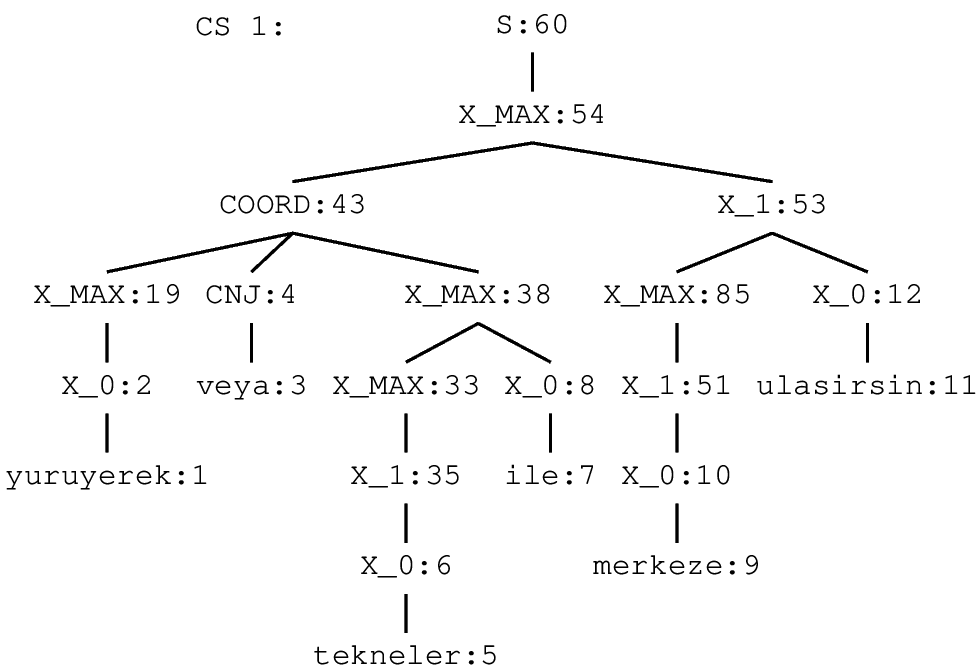
\includegraphics[width=0.72\linewidth]{images/implementation/cstr:verbadj}
	\caption{XLE screenshot of c-structure of sentence (\ref{adj-verbaltestb})}
	\label{fig:cstr-vadj}
\end{figure}

\begin{figure}[H]
	\centering
	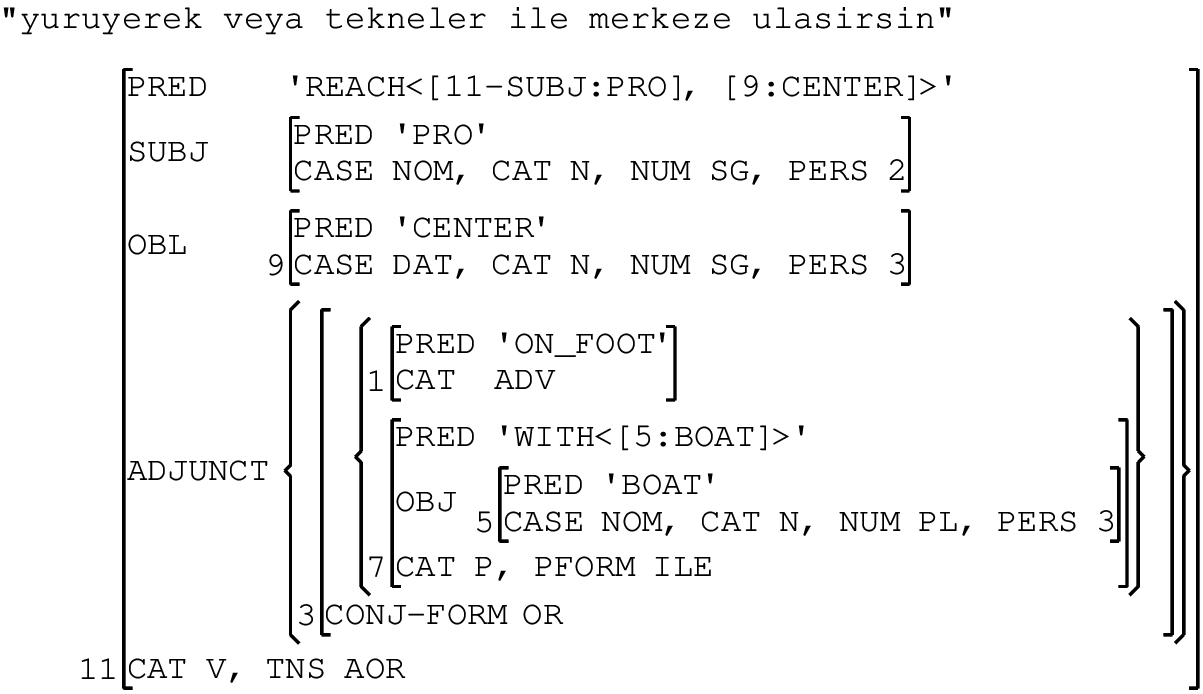
\includegraphics[width=0.7\linewidth]{images/implementation/fstr:verbadj}
	\caption{XLE screenshot of f-structure of sentence (\ref{adj-verbaltestb})}
	\label{fig:fstrverbadj}
\end{figure}

\subsection{Nominal adjuncts}

\begin{sloppypar}
The implementation of the rule governing nominal adjuncts is structurally quite similar to the one for verbal adjuncts, as both types of adjuncts are constrained through their c-structure positions. The rule proposed in the analysis chapter (repeated here in (\ref{imp:adjnom_rule2})) is transferred to XLE as shown in (\ref{imp:adjnomrulexle}). In this rule, the head of the phrase is constrained to be a nominal, as indicated by \mbox{\texttt{(!\ CAT) =c N}}, and the adjuncts can only be either a PP or an AdjP, as indicated by \mbox{\texttt{(!\ CAT) \$ \{P A\}}}.
\end{sloppypar}

\pex
\vspace{-13pt}

\label{imp:adjnom_rule2}
\begin{tabular}{lccc}
	X$'$ & $\longrightarrow$ & XP$^{+}$ & X$'$ \\
	& & $\downarrow$ $\in$ ($\uparrow$ \textsc{adj}) & $\uparrow$ = $\downarrow$ \\
	&			   & ($\downarrow$ \textsc{cat}) $\in_{c}$ \{P, Adj\} & ($\downarrow$ \textsc{cat}) =$_{c}$ N  
\end{tabular}
\xe

\newpage 
\pex
\vspace{-19pt}
\label{imp:adjnomrulexle}

\lstset{
	escapeinside={(*@}{@*)}, basicstyle=\small\ttfamily
}
\begin{lstlisting}
	X_MAX --> {	"NP"
		        {
			"Nominal adjuncts"
			(COORD:! $ (^ ADJUNCT)
				 (! CAT) $ {P A})
			|
			(X_MAX: ! $ (^ ADJUNCT)
				 (! CAT) $ {P A})		
		        }
		        "Nominal head"
		        X_1: ^=!
		             (! CAT) =c N }
	\end{lstlisting}
	\xe

Let us now test this rule on different configurations provided in (\ref{adj-nominaltest}). The first sentence (\ref{adj-nominaltesta}) is ungrammatical because the nominal adjunct position is occupied by a coordination of AdjP and AdvP, which is not permitted according to the rule. However, the sentence (\ref{adj-nominaltestb}) incorporates a coordination of a PP and an AdjP, which should be correctly parsed by the grammar. Finally, the last sentence involves a coordination of AdjPs, which should also not pose a problem for the grammar.

\pex[glspace=!1em,everygla={},everyglb={},aboveglbskip=-.15ex, interpartskip=15pt]
\label{adj-nominaltest}
\a\label{adj-nominaltesta} 
\begingl
\gla\ljudge{*}Güzel ve profesyonel-ce eser-ler-i konuş-tu-k. //
\glb beautiful and professional-\text{advz} work-\textsc{pl}-\textsc{acc} talk-\textsc{pst}-\textsc{1pl} //
\glft `(We) talked about beautiful and professionally works of art.' //
\endgl
\a\label{adj-nominaltestb} 
\begingl
\gla Antik dönem-e ait ve eskimiş eser-ler-i konuş-tu-k. //
\glb antiquated era-\textsc{dat} {belong to} and obsolescent work-\textsc{pl}-\textsc{acc} talk-\textsc{pst}-\textsc{1pl} //
\glft `(We) talked about works of art that belong to ancient history and are obsolescent' //
\endgl
\a\label{adj-nominaltestc} 
\begingl
\gla Güzel ve antik enstrüman-lar-ı konuş-tu-k. //
\glb beautiful and antiquated instrument-\textsc{pl}-\textsc{acc} talk-\textsc{pst}-\textsc{1pl}  //
\glft `(We) talked about beautiful and antiquated instruments.' //
\endgl
\xe 

The first sentence (\ref{adj-nominaltesta}) does not receive a parsing solution, as the nominal adjunct position is occupied by a coordination of an AdjP and an AdvP, which is not permitted. The second sentence (\ref{adj-nominaltestb}) receives the desired parsing solution, as indicated by its c-structure (Figure \ref{fig:cstr-nomadj1}) and f-structure (Figure \ref{fig:fstrnomadj1}).\footnote{The grammar produces another solution for (\ref{adj-nominaltestb}) where \textit{antik} `antiquated' is parsed as one of the conjuncts rather than the adjectival modifier of \textit{döneme} `era'. This alternative reading is indeed easily recoverable in spoken language if a prosodic break (i.e., a pause) is inserted between \textit{antik} and \textit{döneme}.} The last sentence (\ref{adj-nominaltestc}) is also correctly parsed.


\begin{figure}[H]
	\centering
	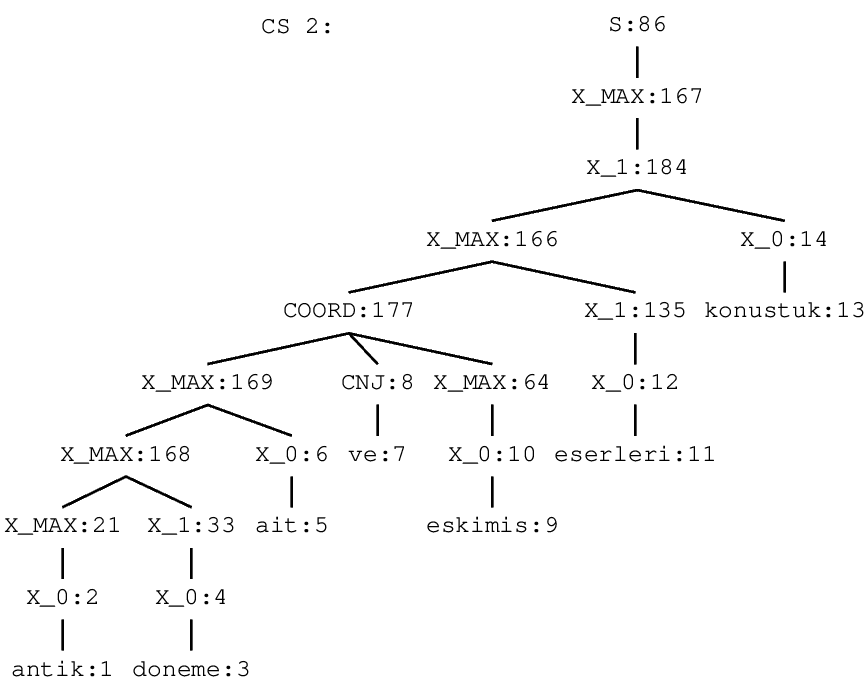
\includegraphics[width=0.7\linewidth]{images/implementation/cstr:nomadj1}
	\caption{XLE screenshot of c-structure of sentence (\ref{adj-nominaltestb})}
	\label{fig:cstr-nomadj1}
\end{figure}

\begin{figure}[H]
	\centering
	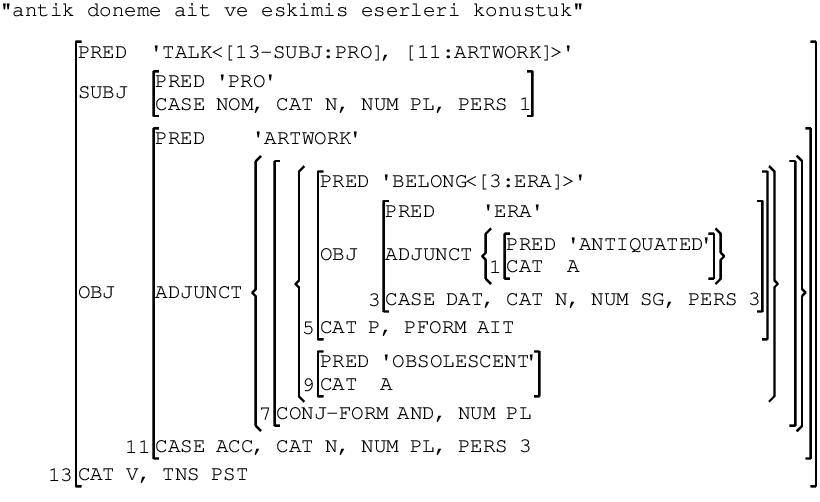
\includegraphics[width=0.73\linewidth]{images/implementation/fstr:nomadj1}
	\caption{XLE screenshot of f-structure of sentence (\ref{adj-nominaltestb})}
	\label{fig:fstrnomadj1}
\end{figure}

\section{Implementing the conservative solution}
\subsection{Off-path constraints}

In the preceding chapter, among the analyses offered by \citeauthor{prz:pat:21:oup}, the choice was made to embrace the liberal solution when formally analyzing Turkish unlike coordination, due to its conceptual advantages. In contrast to the liberal solution, the conservative solution offers the capacity to enforce morphosyntactic constraints on the f-structure of individual conjuncts without extending the formalism of LFG. While the conservative solution involves more complicated formal machinery, it is fully compatible with XLE, making it the ideal option for implementation.

The conservative solution relies on using a specific constraint type called off-path constraints. Before demonstrating their application, consider the examples (\ref{offpath1}) and (\ref{offpath2}) to understand the basic mechanism of off-path constraints on f-structures.

\noindent
\begin{minipage}{0.5\textwidth}
	\pex
	\label{offpath1}
	\a\label{offpath1.constraint}($\uparrow$ \qquad \textsc{a} \qquad \textsc{b} \hspace{5pt} \textsc{c}) =$_{c}$ $+$ \\ \hspace*{0.75em} ($\leftarrow$ \textsc{d}) =$_{c}$ \textsc{e}  
	\a\label{offpath1.fstructure}\begin{avm}
		\[ A \quad \[ 
		B \quad \[ 
		C & + \] 
		\] \\
		D \quad E
		\]
	\end{avm}
	\xe
\end{minipage}
\hfill
\begin{minipage}{0.5\textwidth}
	\pex
	\label{offpath2}
	\a\label{offpath2.constraint}($\uparrow$ \qquad \textsc{a} \qquad \textsc{b} \hspace{5pt} \textsc{c}) =$_{c}$ $+$ \\ \hspace*{0.75em} ($\rightarrow$ \textsc{d}) =$_{c}$ \textsc{e} 
	\a\label{offpath2.fstructure}
	\begin{avm}
		\[ A \quad \[ 
		B \quad \[ 
		C & + \] \\
		D \quad E 
		\]
		
		\]
	\end{avm}
	\xe
\end{minipage}

The constraints themselves can be observed in (\ref{offpath1.constraint}) and (\ref{offpath2.constraint}). The minimal f-structures that satisfy them are given in (\ref{offpath1.fstructure}) and (\ref{offpath2.fstructure}), respectively. The first lines of the constraints are simply constraining equations. The second lines of the constraints, however, are where the off-path constraints are found, which are placed directly below the attribute that they apply. 

Crucially, off-path constraints use distinct metavariables in the form of horizontal arrows. The left arrow ($\leftarrow$) denotes the f-structure that contains the attribute that the off-path constraint applies. The right arrow ($\rightarrow$), on the other hand, refers to the the value of the attribute that the off-path constraint applies. 

In both examples, although the off-path constraint is assigned to the attribute \textsc{a}, they use different horizontal arrows. In (\ref{offpath1.constraint}), the use of $\leftarrow$ states that there must be an attribute-value pair $\langle$\textsc{d, e}$\rangle$ in the f-structure that contains the attribute \textsc{a}, which is satisfied by the f-structure in (\ref{offpath1.fstructure}). In (\ref{offpath2.constraint}), $\rightarrow$ that the attribute-value pair $\langle$\textsc{d, e}$\rangle$ must instead be found in the f-structure that corresponds to the value of the attribute \textsc{a}.

\subsubsection{From distributive statements to off-path constraints}

As previously discussed, he liberal solution proposed by P\&P involves extending the definition of distributivity to constraining statements. The original statement that they proposed for the constraints imposed by \textit{believe} on its oblique argument is shown again in (\ref{przpat:statement1}).

\ex
\label{przpat:statement1}
($\uparrow$ \textsc{obl}) = \%\textsc{c} $\land$ \\
\vspace{3pt}\text{[[}(\%\textsc{c cat}) =$_c$ V $\land$ (\%\textsc{c comp-form}) =$_c$ \textsc{that}] $\lor$ \\
\text{[}(\%\textsc{c cat}) =$_c$ P $\land$ (\%\textsc{c pform}) =$_c$ \textsc{in}\text{]]}
\xe

This statement can be ``translated'' to an off-path constraint to achieve the same effect, as shown below.


\ex
( $\uparrow$  \textsc{obl} \hspace*{9em} \textsc{pred} \hspace*{9.5em}) \\
\hspace*{3em} \{($\leftarrow$ \textsc{cat}) =$_{c}$ V \hspace*{0.5em} $\land$ \hspace*{0.5em} [($\leftarrow$ \textsc{comp-form}) =$_{c}$ \textsc{that} \\
\hspace*{4em} $\lor$ [($\leftarrow$ \textsc{cat}) =$_{c}$ P \hspace*{0.5em} $\land$ \hspace*{0.5em} ($\leftarrow$ \textsc{pform}) =$_{c}$ \textsc{in}]
\xe

Within the context of this off-path constraint, $\leftarrow$ refers to the f-structure of the oblique argument of \textit{believe}. Once this off-path constraint is added to lexical entry for \textit{believe}, the \textsc{obl} argument of \textit{believe} can be either a CP projected by \textit{that}, as indicated by the \textsc{comp-form} attribute, or a PP projected by \textit{in}, as indicated by the \textsc{pform} attribute. The constraint is anchored to the \textsc{pred} attribute, as any lexical item mapped to the \textsc{obl} attribute inherently carries its respective \textsc{pred} attribute. This anchoring ensures that the off-path constraint is evaluated for each f-structure containing \textsc{pred} if the \textsc{obl} attribute is mapped to a hybrid object corresponding to coordination. In other words, this constraint is recycled for each conjunct, as each conjunct has the \textsc{pred} attribute. 


\section{Coordination of unlike arguments}
\subsection{Predicative arguments}

In the previous chapter, the morphosyntactic restrictions imposed by the Turkish verb \textit{ol-} 'be/become' upon its predicative arguments were formulated as a distributive constraint (see (\ref{pred-liberal})). This distributive formulation can be converted into an off-path constraint, as demonstrated in (\ref{pred-offpath}).

\ex
\label{pred-liberal}
($\uparrow$ \textsc{predlink}) = \%\textsc{c} $\land$ \\
\vspace{3pt}\text{[[}(\%\textsc{c cat}) =$_c$ N $\land$ $\neg$\text{[}(\%\textsc{c case}) =$_c$ \textsc{acc} $\lor$ (\%\textsc{c case}) =$_c$ \textsc{dat}\text{]]} $\lor$ \\
(\%\textsc{c cat})  =$_c$ P $\lor$ \\
(\%\textsc{c cat})  =$_c$ Adj\text{]]}
\xe

\ex
\label{pred-offpath}
( $\uparrow$  \textsc{predlink} \hspace*{12em} \textsc{pred} \hspace*{12.8em}) \\
\hspace*{5.3em} \{($\leftarrow$ \textsc{cat}) =$_{c}$ N \hspace*{0.4em} $\land$ \hspace*{0.4em} $\neg$[($\leftarrow$ \textsc{case}) =$_{c}$ \textsc{acc} \hspace*{0.2em} $\lor$ \hspace*{0.2em} ($\leftarrow$ \textsc{case}) =$_{c}$ \textsc{dat}]\}
\\
\hspace*{9.5em} $\lor$ \hspace*{0.4em} [($\leftarrow$ \textsc{cat}) =$_{c}$ P \hspace*{0.4em} $\lor$ \hspace*{0.4em} ($\leftarrow$ \textsc{cat}) =$_{c}$ Adj]
\xe

This off-path constraint states that for each \textsc{pred} containing f-structure that is the value of the \textsc{predlink} attribute, exactly one of the following conditions must be satisfied:

\begin{itemize}
	\item It must contain a \textsc{cat} attribute with the value N (representing nominal category), and it must \textbf{not} possess the attribute-value pairs $\langle$\textsc{case, acc}$\rangle$ or $\langle$\textsc{case, dat}$\rangle$.
	\item It must contain a \textsc{cat} attribute with the value P (representing postpositional category).
	\item It must contain a \textsc{cat} attribute with the value Adj (representing adjectival category).
\end{itemize}

The XLE implementation of the constraint, as shown in (\ref{imp:xleol}), utilizes specific notations to represent various linguistic features. Notably, XLE employs the notation \texttt{<-} to signify the leftward pointing horizontal arrow ($\leftarrow$), establishing the connection between the f-structure(s) and the \textsc{predlink} argument. Additionally, the negation symbol ``$\neg$'' is represented in XLE using the tilde symbol ``$\sim$''. As previously mentioned, XLE interprets the adjacency (as indicated by the space) between statements as an indication of logical conjunction, which renders \mbox{``($\leftarrow$ \textsc{cat}) =${c}$ N''} and \mbox{``$\neg$[($\leftarrow$ \textsc{case}) =${c}$ \textsc{acc} $\lor$ ($\leftarrow$ \textsc{case}) =$_{c}$ \textsc{dat}''} as logical conjuncts. Furthermore, the entire disjunctive constraint is anchored to the \texttt{PRED} attribute through the use of a semicolon adjacent to the \texttt{PRED} attribute.
\newpage
\pex
\vspace{-20pt}
\label{imp:xleol}

\lstset{
	escapeinside={(*@}{@*)}, basicstyle=\small\ttfamily
}

\begin{lstlisting}
    (^ PREDLINK PRED: 
    {(<- CAT) =c N ~{(<- CASE) =c ACC | (<- CASE) =c DAT} | 
    (<- CAT) =c P | 
    (<- CAT) =c A}).
\end{lstlisting}
\xe


This constraint has demonstrated its effectiveness in handling distinct configurations represented by a total of specifically designed 9 test sentences. For well-formed sentences, the grammar correctly provides valid parses, and, in the case of ill-formed strings, the grammar behaves as expected by not providing any solutions.

\subsection{Object arguments}

The verb \textit{konuş-} `talk/converse' imposes intricate morphosyntactic constraints on its object(s). These constraints were captured in the preceding chapter using the subsequent distributive constraining statement:

\ex
\label{obj-liberal}
($\uparrow$ \textsc{obj}) = \%\textsc{c} $\land$ \\
\vspace{3pt}\text{[[}(\%\textsc{c cat}) =$_c$ P $\land$ \text{[}(\%\textsc{c pform}) =$_c$ \textsc{hakkinda} $\lor$ (\%\textsc{c pform}) =$_c$ \textsc{üzerine}\text{]]} $\lor$ \\
\text{[}(\%\textsc{c cat}) =$_c$ N $\land$ \text{[}(\%\textsc{c case}) =$_c$ \textsc{acc} $\lor$ (\%\textsc{c case}) =$_c$ \textsc{nom}\text{]]]}
\xe

This constraining statement can be equivalently transformed into the following off-path constraint:

\ex
\label{obj-conservative}
( $\uparrow$  \textsc{obj} \hspace*{12em} \textsc{pred} \hspace*{16em})
\\
\hspace*{1.5em} [($\leftarrow$ \textsc{cat}) =$_{c}$ P \hspace*{0.2em} $\land$ [($\leftarrow$ \textsc{pform}) =$_{c}$ \textsc{hakkında} $\lor$ \hspace*{0.2em} ($\leftarrow$ \textsc{pform}) =$_{c}$ \textsc{üzerine}]] \\
\hspace*{3.5em} $\lor$  \{($\leftarrow$ \textsc{cat}) =$_{c}$ N \hspace*{0.2em} $\land$ \hspace*{0.2em} [($\leftarrow$ \textsc{case}) =$_{c}$ \textsc{acc} $\lor$ ($\leftarrow$ \textsc{case}) =$_{c}$ \textsc{nom}]\} 
\xe

This off-path constraint stipulates that for each \textsc{pred} containing f-structure that is the value of the \textsc{obj} attribute, exactly one of the following constraints must hold:

\begin{sloppypar}
	\begin{itemize}
		\item It must contain a \textsc{cat} attribute with the value P, and it must either possess the attribute-value pair $\langle$\textsc{pform, hakkında}$\rangle$ or $\langle$\textsc{pform, üzerine}$\rangle$.
		\item It must contain a \textsc{cat} attribute with the value N, and it must possess either the attribute-value pair $\langle$\textsc{case, acc}$\rangle$ or $\langle$\textsc{case, nom}$\rangle$.
	\end{itemize}
\end{sloppypar}

The corresponding XLE implementation of this constraint is presented below:

\pex
\label{imp:xlekonuş_modified}
\vspace{-18pt}

\lstset{
	escapeinside={(*@}{@*)}, basicstyle=\small\ttfamily
}
\begin{lstlisting}
    (^ OBJ PRED:
    {(<- CAT) =c N {(<- CASE) =c ACC | (<- CASE) =c NOM} |
    (<- CAT) =c P {(<- PFORM) =c HAKKINDA 
    | (<- PFORM) =c UZERINE}}).
\end{lstlisting}
\xe

The effectiveness of this constraint was verified through testing on 8 different configurations (sentences), where it demonstrated its capability to handle them effectively.

\subsection{Oblique arguments}

Coordination uf unlike oblique arguments was examined in the previous chapter within the context of two verbs: \textit{saydır-} `curse/swear' and sür- `last/continue'.

The morphosyntactic constraints imposed by the verb \textit{saydır-} on its oblique argument was formulated through the distributive statement in (\ref{obl-liberal}), which is translated into the off-path constraint in (\ref{obl-cons}).

\ex
\label{obl-liberal}
($\uparrow$ \textsc{obl}) = \%\textsc{c} $\land$ \\
\vspace{3pt}\text{[[}(\%\textsc{c cat}) =$_c$ N $\land$ (\%\textsc{c case}) =$_c$ \textsc{dat}\text{]} $\lor$ \\
\text{[}(\%\textsc{c cat}) =$_c$ P $\land$ (\%\textsc{c pform}) =$_c$ \textsc{hakkinda}\text{]]}
\xe

\ex
\label{obl-cons}
( $\uparrow$  \textsc{obl} \hspace*{8em} \textsc{pred} \hspace*{11.3em}) \\
\hspace*{6.2em} [($\leftarrow$ \textsc{cat}) =$_{c}$ N \hspace*{.4em} $\land$ \hspace*{.4em} ($\leftarrow$ \textsc{case}) =$_{c}$ \textsc{dat}] \\
\hspace*{3.5em} $\lor$ [($\leftarrow$ \textsc{cat}) =$_{c}$ P \hspace*{.4em} $\land$ \hspace*{.4em} ($\leftarrow$ \textsc{pform}) =$_{c}$ \textsc{hakkında}]
\xe

This off-path constraint states that for each \textsc{pred} containing f-structure that is the value of the attribute \textsc{obl}, exactly one of the following constraints must hold:

\begin{itemize}
\item It must contain a \textsc{cat} attribute with the value N, and it must possess the attribute-value pair $\langle$\textsc{case, dat}$\rangle$.
\item It must contain a \textsc{cat} attribute with the value P, and it must possess the attribute-value pair $\langle$\textsc{pform, hakkında}$\rangle$.

\end{itemize}

The XLE version of this constraint is provided in (\ref{imp:xlesaydir}). This constraint was tested on 8 distinct configurations and effectively handled both well-formed and ill-formed strings.

\pex
\label{imp:xlesaydir}
\vspace{-18pt}

\lstset{
	escapeinside={(*@}{@*)}, basicstyle=\small\ttfamily
}
\begin{lstlisting}
    (^ OBL PRED: 
    {(<- CAT) =c N (<- CASE) =c DAT | 
    (<- CAT) =c P (<- PFORM) =c HAKKINDA}).
\end{lstlisting}
\xe

Turning our attention to the verb \textit{sür-}, its constraints pertaining to its \textsc{obl} argument(s) were formulated in the form of a distributive statement in the previous chapter as presented below:

\ex
\label{sur-liberal}
($\uparrow$ \textsc{obl}) = \%\textsc{c} $\land$ \\
\vspace{3pt}\text{[[}(\%\textsc{c cat}) =$_c$ N $\land$ (\%\textsc{c case}) =$_c$ \textsc{nom}\text{]} $\lor$ \\
\text{[}(\%\textsc{c cat}) =$_c$ P $\land$ (\%\textsc{c pform}) =$_c$ \textsc{boyunca}\text{]} $\lor$ \\
(\%\textsc{c cat}) =$_c$ Adv\text{]}
\xe

The off-path constraint equivalent of this distributive formulation is provided below:

\ex
\label{sur-cons}
( $\uparrow$  \textsc{obl} \hspace*{6em} \textsc{pred} \hspace*{9.8em}) \\
\hspace*{3.2em} [($\leftarrow$ \textsc{cat}) =$_{c}$ N \hspace*{.4em} $\land$ \hspace*{.4em} ($\leftarrow$ \textsc{case}) =$_{c}$ \textsc{nom}] \\
\hspace*{.9em} $\lor$ [($\leftarrow$ \textsc{cat}) =$_{c}$ P \hspace*{.4em} $\land$ \hspace*{.4em} ($\leftarrow$ \textsc{pform}) =$_{c}$ \textsc{boyunca}] \\
\hspace*{.9 em} $\lor$ ($\leftarrow$ \textsc{cat}) =$_{c}$ Adv
\xe

This off-path constraint states that for each \textsc{pred} containing f-structure that is the value of the attribute \textsc{obl}, exactly one of the following constraints must hold:

\begin{itemize}
	\item It must contain a \textsc{cat} attribute with the value N, and it must possess the attribute-value pair $\langle$\textsc{case, nom}$\rangle$.
	\item It must contain a \textsc{cat} attribute with the value P, and it must possess the attribute-value pair $\langle$\textsc{pform, boyunca}$\rangle$.
	\item It must contain a \textsc{cat} attribute with the value Adv.
\end{itemize}

The corresponding XLE implementation of this constraint, demonstrated in (\ref{imp:xlesaydir}), was tested on 12 distinct configurations, successfully handling both well-formed and ill-formed strings.

\pex
\label{imp:xlesur}
\vspace{-20pt}

\lstset{
	escapeinside={(*@}{@*)}, basicstyle=\small\ttfamily
}
\begin{lstlisting}
    (^ OBL PRED: 
    {(<- CAT) =c N (<- CASE) =c NOM | 
    (<- CAT) =c P (<- PFORM) =c BOYUNCA |
    (<- CAT) =c ADV}).
\end{lstlisting}
\xe

\section{Conclusion}

This chapter provided an overview of the XLE implementation of the proposed analysis from the preceding chapter. The success of the implementation is ensured through rigorous testing involving 53 sentences. The `conservative solution' proposed by \citeauthor{prz:pat:21:oup} enables the representation of intricate morphosyntactic constraints associated with specific verbs while maintaining full XLE compatibility.

\begin{sloppypar}
An especially noteworthy accomplishment of this implementation is the effective transfer of syntactic category information from node labels to the f-structure. This accomplishment not only validates the viability of the analysis proposed by \citeauthor{prz:pat:21:oup}, but also underscores the versatility of the LFG and XLE framework. 
\end{sloppypar}
	\chapter{Conclusion} \label{ch:conclusion}
	\begin{sloppypar}
To the best of this author's knowledge, this thesis constitutes the first attempt at investigating unlike coordination phenomena in Turkish. To maximize scientific validity, two widely employed methodologies in linguistics were utilized: corpus study and acceptability judgment study. Furthermore, these methodologies were employed in a way that complemented each other.
\end{sloppypar}

The results from both the corpus study and the acceptability judgment task provide compelling evidence that Turkish indeed allows for coordination of unlike elements, both in terms of unlike category and unlike case coordination. However, unlike coordination in Turkish is subject to certain restrictions; not all elements can be coordinated with one another. The grammatical function of the conjuncts appears to play a significant role in determining the acceptability of such structures, as hypothesized at the outset of the thesis. This hypothesis finds strong support both in the corpus study and acceptability judgment task. In the corpus study, the vast majority of examples feature conjuncts with matching functions. Additionally, the linear-mixed effects models applied to the acceptability judgment task data further confirm this observation, as mismatching functions were found to be a negative predictor of acceptability ratings. 


In conclusion, the empirical investigations confirm the hypothesis put forward in this research, also providing support for the increasingly prevalent view that coordination does not universally require conjuncts to match in their morphosyntactic properties. However, further empirical data from other languages would indeed be valuable in strengthening this position.

To analyze and formalize the observed empirical facts, the thesis adopts the framework of Lexical-Functional Grammar and follows the approach proposed by \citet{prz:pat:21:oup}. The analysis refrains from encoding an overarching principle that only conjuncts with like functions can be coordinated, as was suggested by \citet{peterson2004}. Instead, it proposes that each conjunct must meet certain constraints within the syntactic position they occupy, which is a position aligned with \citet{prze:22:cases}. Consequently, this approach elegantly accounts for the empirical observations on Turkish coordination without postulating Turkish- or coordination-specific parameters.

Furthermore, the implementation chapter demonstrates that the proposed analysis of unlike coordination can be implemented. The logic behind the implementation was determined to be straightforward and fully compatible with XLE. However, a noteworthy challenge that requires further investigation involves integrating an approach that transfers syntactic categories from c-structure to f-structure within existing XLE implementations and grammar engineering frameworks. 

	% Bibliography %

	\bibliographystyle{apalike}
	\bibliography{library.bib}
	
	% Appendix %

	\appendix
	\clearpage
	\chapter{Corpus study} \label{appx:corpus_study}
	\section{CQL queries} \label{app:cqlqueries}

\subsection{Interpreting CQL queries}

CQL is a specialized language used for querying and searching linguistic data within a corpus. Queries in CQL are written in a code-like format and consist of several components, each serving a specific purpose:\\
\begin{sloppypar}
\noindent \textbf{Tags and tag patterns:} Tags represent specific parts of speech (e.g., nouns, verbs, adjectives) and are enclosed in angle brackets (< >). Tag patterns can match multiple sub-types associated with a tag, which can be achieved by an asterisk symbol. For example, the block, \Verb"[tag=`<Postp[:>].*']", targets all types of tokens as long as they are tagged as postpositions. The block \mbox{\Verb"[longtag=`<Det:indef>']"}, however, targets only indefinite determiners, which is a sub-type of determiners. The blocks that target sub-types use the keyword \Verb"longtag" and omit the asterisk symbol.\\
\end{sloppypar}
\noindent \textbf{Optional elements:} Optional elements in the query are denoted by placing a question mark (?) after the element. These elements may or may not be present in the pattern being searched. For instance, the block, \Verb"[tag=`Det:indef']?" specifies that this position can be optionally filled by an indefinite determiner.\\

\noindent \textbf{Exclusion:} The ``!='' symbol is used to exclude specific tags or patterns from the query, ensuring that certain elements are not present in the sentence. For example, the block, \Verb"[tag!=`<V[:>].*']", fails to match if the position is filled by any verbal element.\\

\begin{sloppypar}
	\noindent \textbf{Logical operators:} Logical operators such as ``\&'' (AND) and ``|'' (OR) are used to combine different elements within the query and impose more sophisticated requirements on the patterns. For instance, the block \Verb"[tag=`<N[:>].*' & tag!=`<N><sg>']" targets non-singular nouns in the corpus.
\end{sloppypar}

\noindent \textbf{Coordinating conjunction:} The presence of a coordinating conjunction is indicated using the \Verb"Cnj:coo" longtag, representing conjunctions like \textit{and} or \textit{or}. \\

\noindent \textbf{Stem:} The \Verb"stem" attribute allows specific verb stems to be targeted, enabling the search for patterns incorporating particular verb forms. For instance, the block, \Verb"[tag=`<V[:>].*' & stem=`run']", targets all verbs with the stem \textit{run}.\\

\noindent \textbf{Word search:} Specific words can be targeted using the \Verb"word" attribute, allowing searches for patterns containing specific lexical items. For example, the block, \Verb"[word=`alien']", matches the word ``alien.''\\

The linear order of elements in the query directly corresponds to the linear order of elements searched in a sentence pattern. This means that the components in the query are interpreted in the same order they appear, allowing for precise control over the arrangement and occurrence of linguistic elements in the targeted patterns.

\subsection{Coordination of unlike categories}
\subsubsection{PP \& NP}

\begin{figure}[!h]
	\lstset{
		escapeinside={(*@}{@*)},basicstyle=\footnotesize\ttfamily
	}
	\begin{lstlisting}
[tag!="<V[:>].*"] [longtag="<Det:indef>"]?[tag="<Adj[:>].*"]?
[tag="<N[:>].*"] [tag="<Postp[:>].*"] [longtag="<Cnj:coo>"]
[tag="<Adj[:>].*"]? [longtag="<Det:indef>"]? [tag="<N[:>].*"]
[tag!="<Postp[:>].*"]
		\end{lstlisting}
	\caption{General PP \& NP Query}
	\label{CQl_ppnp-general}
\end{figure}


\begin{figure}[!h]
		\lstset{
	escapeinside={(*@}{@*)},basicstyle=\footnotesize\ttfamily
}
	\begin{lstlisting}
[tag!="<V[:>].*"] [tag="<Adj[:>].*"]? [longtag="<Det:indef>"]? 
[tag="<N[:>].*"] [tag="<Postp[:>].*"] [longtag="<Cnj:coo>"]
[tag="<Adj[:>].*"]? [longtag="<Det:indef>"]? [tag="<N[:>].*"]
[stem="ol" & tag="<V[:>].*"][tag!="<Postp[:>].*"]
	\end{lstlisting}
	\caption{PP \& NP \textsc{to be} Query}
	\label{CQl_ppnp-olmak}
\end{figure}


\begin{figure}[!h]
		\lstset{
	escapeinside={(*@}{@*)},basicstyle=\footnotesize\ttfamily
}
		\begin{lstlisting}
[tag="<Adj[:>].*"]? [longtag="<Det:indef>"]? [tag="<N[:>].*"]
[tag="<Postp[:>].*"] [longtag="<Cnj:coo>"] [tag="<Adj[:>].*"]?
[longtag = "<Det:indef>"]? [tag="<N[:>].*"] [tag!="<Postp[:>].*"] 
[tag="<V[:>].*" & stem="dusun"]
		\end{lstlisting}
	\caption{PP \& NP \textsc{to think/consider} Query}
	\label{CQl_ppnp-düşünmek}
\end{figure}

The query in Figure \ref{CQl_ppnp-konuşmak} additionally specifies that the postpositional head of the first conjunct may alternatively be occupied by the word \textit{hakkında} `about'. This stems from the fact that the automatic POS-tagger employed in the corpus sometimes tags \textit{hakkında} as a locative noun even though it was classified as a type of postposition by \citet[pp.\ 100--102]{kornfilt97}.

\begin{figure}[!h]
		\lstset{
	escapeinside={(*@}{@*)},basicstyle=\footnotesize\ttfamily
		}
		\begin{lstlisting}
[tag!="<V[:>].*"] [tag="<Adj[:>].*"]? [longtag="<Det:indef>"]?
[tag="<N[:>].*"] [tag="<Postp[:>].*" | word="hakkinda"]
[tag="<Cnj:coo>"][tag="<Adj[:>].*"]? [longtag="<Det:indef>"]?
[tag="<N[:>].*"][tag!="<Postp[:>].*"] 
[tag="<V[:>].*" & stem="konus"]
		\end{lstlisting}
	\caption{PP \& NP \textsc{to talk/converse/speak} Query}
	\label{CQl_ppnp-konuşmak}
\end{figure}

\newpage
\subsubsection{PP \& AdvP}

\begin{figure}[!h]
		\lstset{
			escapeinside={(*@}{@*)},basicstyle=\footnotesize\ttfamily
		}
		\begin{lstlisting}
[tag="<Adj[:>].*"]? [longtag="<Det:indef>"]? [tag="<N[:>].*"]
[tag="<Postp[:>].*"] [longtag="<Cnj:coo>"] [tag="<Adv[:>].*"]
[tag="<V[:>].*"]
		\end{lstlisting}
	\caption{General PP \& AdvP Query}
	\label{CQl_pp-advpgeneral}
\end{figure}

\subsubsection{PP \& AdjP}

\begin{figure}[!h]
	\lstset{
		escapeinside={(*@}{@*)},basicstyle=\footnotesize\ttfamily
	}
	\begin{lstlisting}
[tag="<Adj[:>].*"]? [tag="<Det:indef>"]? [tag="<N[:>].*"]
[tag="<Postp[:>].*"] [longtag="<Cnj:coo>"] [tag = "<Adv[:>].*"]?
[tag = "<Adj[:>].*"] [tag="<V[:>].*"]
	\end{lstlisting}
	\caption{General PP \& AdjP Query}
	\label{CQl_pp-adjpgeneral}
\end{figure}


\subsubsection{NP \& AdjP}

\begin{figure}[!h]
	\lstset{
		escapeinside={(*@}{@*)},basicstyle=\footnotesize\ttfamily
	}
	\begin{lstlisting}
[tag != "<V[:>].*"][tag = "<Adj[:>].*"]?[tag = "<Det:indef>"]?
[tag = "<N[:>].*"] [longtag = "<Cnj:coo>"][tag = "<Adv[:>].*"]?
[tag = "<Adj[:>].*"][stem= "ol" & tag= "<V[:>].*"]
	\end{lstlisting}
	\caption{NP \& AdjP \textsc{to be} Query}
	\label{CQl_np-adjptobe}
\end{figure}

\subsubsection{NP \& AdvP}

\begin{figure}[!h]
	\lstset{
		escapeinside={(*@}{@*)},basicstyle=\footnotesize\ttfamily
	}
	\begin{lstlisting}
[tag!="<V[:>].*"] [tag="<Num>"]?[tag="<N[:>].*"] [longtag="<Cnj:coo>"] 
[tag="<Adv[:>].*"] [tag="<V[:>].*" & stem="sur"]
	\end{lstlisting}
	\caption{NP (numerical) \& AdvP \textsc{to last} Query}
	\label{CQl_np-advplast}
\end{figure}

\begin{figure}[!h]
	\lstset{
		escapeinside={(*@}{@*)},basicstyle=\footnotesize\ttfamily
	}
	\begin{lstlisting}
[tag!="<V[:>].*"][tag="<Adj[:>].*"]? [longtag=``<Det:indef>'']?
[tag="<N[:>].*"] [longtag="<Cnj:coo>"] [tag="<Adv[:>].*"]
[tag="<V[:>].*" & stem="hallet"] 
	\end{lstlisting}
	\caption{NP \& AdvP \textsc{to handle} Query}
	\label{CQl_np-advphallet}
\end{figure}

\newpage

\subsection{Coordination of unlike cases}

\begin{figure}[!h]
	\lstset{
		escapeinside={(*@}{@*)},basicstyle=\footnotesize\ttfamily
	}
	\begin{lstlisting}
[tag != "<V[:>].*"] [tag = "<Adj[:>].*"]? 
[longtag = "<Det:indef>"]? [(longtag = "<N><dat>") | 
(longtag = "<N><gen>" | longtag = "<N><abl>") | longtag = "<N><ins>" 
| longtag = "<N><loc>"] [longtag = "<Cnj:coo>"] [tag = "<Adj[:>].*"]? 
[longtag = "<Det:indef>"]? [longtag = "<N><acc>"] 
[tag != "<N[:>].*" & tag != "<Postp[:>].*"]
	\end{lstlisting}
	\caption{NP($\neg$acc) \& NP(acc) Query}
	\label{CQl_npacc}
\end{figure}

\begin{figure}[!h]
	\lstset{
		escapeinside={(*@}{@*)},basicstyle=\footnotesize\ttfamily
	}
	\begin{lstlisting}
[tag != "<V[:>].*"] [tag = "<Adj[:>].*"]? 
[longtag = "<Det:indef>"]? [(longtag = "<N><acc>") | 
(longtag = "<N><gen>" | longtag = "<N><abl>") | longtag = "<N><ins>" 
| longtag = "<N><loc>"] [longtag = "<Cnj:coo>"] [tag = "<Adj[:>].*"]? 
[longtag = "<Det:indef>"]? [longtag = "<N><dat>"] 
[tag != "<N[:>].*" & tag != "<Postp[:>].*"]
	\end{lstlisting}
	\caption{NP($\neg$dat) \& NP(dat) Query}
	\label{CQl_npdat}
\end{figure}

\begin{figure}[!h]
	\lstset{
		escapeinside={(*@}{@*)},basicstyle=\footnotesize\ttfamily
	}
	\begin{lstlisting}
[tag != "<V[:>].*"] [tag = "<Adj[:>].*"]? 
[longtag = "<Det:indef>"]? [(longtag = "<N><acc>") | 
(longtag = "<N><dat>" | longtag = "<N><abl>") | longtag = "<N><ins>" 
| longtag = "<N><loc>"] [longtag = "<Cnj:coo>"] [tag = "<Adj[:>].*"]? 
[longtag = "<Det:indef>"]? [longtag = "<N><gen>"] 
[tag != "<N[:>].*" & tag != "<Postp[:>].*"]
	\end{lstlisting}
	\caption{NP($\neg$gen) \& NP(gen) Query}
	\label{CQl_npgen}
\end{figure}

\begin{figure}[!h]
	\lstset{
		escapeinside={(*@}{@*)},basicstyle=\footnotesize\ttfamily
	}
	\begin{lstlisting}
[tag != "<V[:>].*"] [tag = "<Adj[:>].*"]? 
[longtag = "<Det:indef>"]? [(longtag = "<N><acc>") | 
(longtag = "<N><dat>" | longtag = "<N><abl>") | longtag = "<N><gen>" 
| longtag = "<N><loc>"] [longtag = "<Cnj:coo>"] [tag = "<Adj[:>].*"]? 
[longtag = "<Det:indef>"]? [longtag = "<N><ins>"] 
[tag != "<N[:>].*" & tag != "<Postp[:>].*"]
	\end{lstlisting}
	\caption{NP($\neg$ins) \& NP(ins) Query}
	\label{CQl_npins}
\end{figure}

\begin{figure}[H]
	\lstset{
		escapeinside={(*@}{@*)},basicstyle=\footnotesize\ttfamily
	}
	\begin{lstlisting}
[tag != "<V[:>].*"] [tag = "<Adj[:>].*"]? 
[longtag = "<Det:indef>"]? [(longtag = "<N><acc>") | 
(longtag = "<N><dat>" | longtag = "<N><ins>") | longtag = "<N><gen>" 
| longtag = "<N><loc>"] [longtag = "<Cnj:coo>"] [tag = "<Adj[:>].*"]? 
[longtag = "<Det:indef>"]? [longtag = "<N><abl>"] 
[tag != "<N[:>].*" & tag != "<Postp[:>].*"]
	\end{lstlisting}
	\caption{NP($\neg$abl) \& NP(abl) Query}
	\label{CQl_npabl}
\end{figure}

\begin{figure}[H]
	\lstset{
		escapeinside={(*@}{@*)},basicstyle=\footnotesize\ttfamily
	}
	\begin{lstlisting}
[tag != "<V[:>].*"] [tag = "<Adj[:>].*"]? 
[longtag = "<Det:indef>"]? [(longtag = "<N><acc>") | 
(longtag = "<N><dat>" | longtag = "<N><ins>") | longtag = "<N><gen>" 
| longtag = "<N><abl>"] [longtag = "<Cnj:coo>"] [tag = "<Adj[:>].*"]? 
[longtag = "<Det:indef>"]? [longtag = "<N><loc>"] 
[tag != "<N[:>].*" & tag != "<Postp[:>].*"]
	\end{lstlisting}
	\caption{NP($\neg$loc) \& NP(loc) Query}
	\label{CQl_nploc}
\end{figure}

\section{Valency dictionary} \label{app:valency}
\subsection{Treebanks}

In order to construct the small-scale valency dictionary of Turkish verbs, 5 prominent Turkish dependency treebanks, which are listed in Table \ref{treebanks_table}, have been automatically parsed with a script written in Python (\textit{version} 3.8.12). 

\begin{table}[!h]
	\centering
	\scalebox{0.93}{
		\begin{tabular}{crrcc}
			\textbf{Treebank}                                                    & \textbf{Sentences} & \textbf{Tokens} & \textbf{Annotation} & \textbf{Document Type} \\ \hline \hline
			\textit{\begin{tabular}[c]{@{}c@{}} TWT\footnote{\citealp{twt-treebank}} \end{tabular}} & 4,851              & 80,920          & Manual              & Web                    \\
			\textit{The Grammarbook}\footnote{\citealp{grammarbook-treebank}}                                            & 2,803              & 16,516          & Semi-automatic & Textbook examples      \\
			\textit{IMST-UD}\footnote{\citealp{sulubacak-etal-2016-universal}} & 5,635 & 56,423 & Semi-automatic & \begin{tabular}[c]{@{}c@{}}News reports,\\ novels\end{tabular} \\
			\textit{BOUN}\footnote{\citealp{boun-treebank}}                                                                 & 9,761              & 121,214         & Manual              & Various                \\
			\textit{Kenet UD}\footnote{\href{https://github.com/UniversalDependencies/UD_Turkish-Kenet}{Kenet-UD GitHub Repository}}                                                             & 18,700             & 178,700         & Manual              & Various                \\ \hline
	\end{tabular} }
	\caption{List of treebanks employed in the corpus study}
	\label{treebanks_table}
\end{table}

\subsection{Procedure}
A dedicated Python library named \textit{conllu} (\texttt{https://pypi.org/project/conllu/}) was employed to parse the treebanks encoded in CoNLL--U format. The written script in Python automatically constructed the dictionary entries in the following steps: 1) it extracted the main verb/predicate of a sentence; 2) it identified the dependents of the main verb that serve the role of object, oblique and open clausal complement (xcomp) in their relation to the verb; 3) it catalogued the morphosyntactic properties (case and category) of the identified dependents alongside their respective verbal governors.  

Once the dictionary was constructed, each entry was semi-automatically evaluated. First, a Python script automatically eliminated verbal entries that imposed only one category and case requirement on its argument(s). Subsequently, the remaining entries were manually evaluated and CQL queries were designed for the promising verbs. Most of the designed queries resulted in no verified results. An example entry from the constructed dictionary can be seen in (\ref{valencyentry}), which is the entry for the Turkish verb \textit{bas} (to press/push). 


\pex \label{valencyentry}
\vspace{-2.1em}
\begin{Verbatim}[xleftmargin=-.2in]
	bas (V):
	{
		`ObjCat': {`NOUN'}, `ObjCase': {`Dat', `Acc'}, 
		`OblCat': {`NOUN'}, 'OblCase': {`Dat', `Loc'}, 
		`XCompCat': {`NOUN'}, `XCompCase': {`Dat'}
	}
\end{Verbatim}
\xe

According to (\ref{valencyentry}), \textit{bas} can take three kinds of arguments: \textsc{obj}(ect), \textsc{obl}(ique), and \textsc{xcomp}. While \textsc{obj} function is realised by a dative or an accusative noun, the \textsc{obl} element should either be a dative or a locative noun. \textsc{xcomp} argument, on the other hand, can only be a nominal element in the dative case. 

	\chapter{Acceptability judgment task} \label{appx:acc_experiment}
	\section{Sub-surveys} \label{app:subsurveys}

In the following tables, each cell should be understood as a sentence token that belongs to a particular token set and type based on its row and column indices. For example, the cell whose row name is ``TS-6" and whose column name ``UCAT-LF'' is a sentence token from the token set 6 and represents the type: unlike category like function coordination. A symbol inserted in this cell, which is $\alpha$ in this case, signifies that this sentence is assigned to the survey symbolised as $\alpha$, which is Survey 1. 

\subsection{Category block}

\begin{tabular}{|c|c|c|c|c|}
	\hline
	 & \textbf{LCAT-LF} & \textbf{UCAT-LF} & \textbf{LCAT-UF} & \textbf{UCAT-UF} \\ \hline
	TS-1 & $\alpha$ & $\beta$ & $\gamma$ & $\delta$ \\ \hline
	TS-2 & $\delta$ & $\alpha$ & $\beta$ & $\gamma$ \\ \hline
	TS-3 & $\gamma$ & $\delta$ & $\alpha$ & $\beta$ \\ \hline
	TS-4 & $\beta$ & $\gamma$ & $\delta$ & $\alpha$ \\ \hline
	TS-5 & $\alpha$ & $\beta$ & $\gamma$ & $\delta$ \\ \hline
	TS-6 & $\delta$ & $\alpha$ & $\beta$ & $\gamma$ \\ \hline
	TS-7 & $\gamma$ & $\delta$ & $\alpha$ & $\beta$ \\ \hline
	TS-8 & $\beta$ & $\gamma$ & $\delta$ & $\alpha$ \\ \hline
	TS-9 & $\alpha$ & $\beta$ & $\gamma$ & $\delta$ \\ \hline
	TS-10 & $\delta$ & $\alpha$ & $\beta$ & $\gamma$ \\ \hline
	TS-11 & $\gamma$ & $\delta$ & $\alpha$ & $\beta$ \\ \hline
	TS-12 & $\beta$ & $\gamma$ & $\delta$ & $\alpha$ \\ \hline
\end{tabular}
\quad
\begin{tabular}{|c|c|}
	\hline
	\textbf{Symbol} & \textbf{Survey} \\ \hline
	$\alpha$ & Survey 1 \\ \hline
	$\beta$ & Survey 2 \\ \hline
	$\gamma$ & Survey 3 \\ \hline
	$\delta$ & Survey 4 \\ \hline
\end{tabular}



\subsection{Case block}

\begin{tabular}{|c|c|c|c|}
	\hline
	 & \textbf{LCASE-LF} & \textbf{UCASE-LF} & \textbf{UCASE-UF} \\ \hline
	TS-1 & $\alpha$ & $\delta$ & $\gamma$ \\ \hline
	TS-2 & $\beta$ & $\alpha$ & $\delta$ \\ \hline
	TS-3 & $\gamma$ & $\beta$ & $\alpha$ \\ \hline
	TS-4 & $\delta$ & $\gamma$ & $\beta$ \\ \hline
	TS-5 & $\alpha$ & $\delta$ & $\gamma$ \\ \hline
	TS-6 & $\beta$ & $\alpha$ & $\delta$ \\ \hline
	TS-7 & $\gamma$ & $\beta$ & $\alpha$ \\ \hline
	TS-8 & $\delta$ & $\gamma$ & $\beta$ \\ \hline
	TS-9 & $\alpha$ & $\delta$ & $\gamma$ \\ \hline
	TS-10 & $\beta$ & $\alpha$ & $\delta$ \\ \hline
	TS-11 & $\gamma$ & $\beta$ & $\alpha$ \\ \hline
	TS-12 & $\delta$ & $\gamma$ & $\beta$ \\ \hline
\end{tabular}
\quad
\begin{tabular}{|c|c|}
	\hline
	\textbf{Symbol} & \textbf{Survey} \\ \hline
	$\alpha$ & Survey 1 \\ \hline
	$\beta$ & Survey 2 \\ \hline
	$\gamma$ & Survey 3 \\ \hline
	$\delta$ & Survey 4 \\ \hline
\end{tabular}

\section{Instructions} \label{app:instruct}
\subsection{Turkish original}

\begin{center}
	\large \textbf{Sayfa 1/2}
\end{center}


\textbf{Lütfen ankete başlamadan önce yönergeleri dikkatle okuyunuz ve anladığınıza emin olunuz.}

Bu ankette size ardı ardına farklı Türkçe cümleler gösterilecek. Öncelikle gösterilen cümleyi dikkatle okuyunuz. Ardından bu cümleyi günlük hayatınızda duyduğunuz veya okuduğunuz bir durum hayal etmeye çalışın.

Örnek durumlardan bazıları: 

\begin{itemize}
	\item Sokaktaki birinin bu cümleyi kurmuş olması
	\item Afiş, mesaj, kitapçık, sosyal medya postu veya reklam panolarında okumuş olmanız.
\end{itemize}


\begin{sloppypar}
	
	Kendinizi bu duruma koyduktan sonra, bu cümleye olan dilsel tepkinizi \mbox{(--3) ve (3)} ölçeği üzerinden puanlandırınız. Ölçeğin uç noktaları şöyle yorumlanmalıdır: 
	
\end{sloppypar}

(3): Anadili Türkçe olan biri tarafından kurulmuş gibi duyulan bir cümle. Tamamen doğal ve anlaşılabilir. 



(--3): Anlaşılması oldukça güç (hatta anlam ifade etmeyen), garip duyulan ve Türkçeyi yeni öğrenen bir yabancı tarafından kurulmuş olması oldukça muhtemel.


Eğer gösterilen cümleye olan tepkiniz bu iki uç nokta arasında ise aradaki değerleri tepkinizin derecesine göre kullanınız. Örneğin, oldukça doğal duyulan fakat az da olsa bir gariplik barındıran cümle için (1) veya (2) kullanılabilir. 

\vspace{10pt}
\textbf{
	Anket sırasında verdiğiniz puanlar cümleden cümleye önemli değişiklikler gösterebilir.}

\newpage
\begin{center}
	\large \textbf{Sayfa 2/2}
\end{center}

\textbf{ÖNEMLİ NOKTALAR:}

\begin{itemize}
	\item Bu ankette DOĞRU veya YANLIŞ cevap kavramı bulunmamaktadır. Cümleleri puanlarken okulda öğrenmiş olduğunuz çeşitli dilbilgisi ve yazım kurallarını göz önünde bulundurmayınız. Bu çalışma için önemli olan sizin anadili Türkçe olan biri olarak Türkçenin günlük hayattaki kullanımına dair içgüdüsel yaklaşımınızı tespit etmektir.
	\item Bazı cümlelerin ifade ettiği fikirlere kişisel olarak katılmıyor olabilirsiniz. Fakat bu çalışma için önemli olan cümlelerin ifade ettiklerine karşı olan tutumunuz \textbf{DEĞİL}, cümleleri ne kadar anlaşılabilir ve doğal bulduğunuzdur.
\end{itemize}

\textbf{Bazı örnek cümlelerin değerlendirilmesi:}


Gösterilen bazı cümlelerdeki yazım biçimleri anadili Türkçe olan kişilerin günlük hayattaki konuşmalarını yansıtacak şekilde olabilir. Eğer aşağıdaki cümle size anadili Türkçe olan biri tarafından kurulmuş gibi duyuluyorsa, yazım biçimini görmezden geliniz.

\begin{enumerate}
	\item ``Dersten sonra ananemlere uğrıycam.''
\end{enumerate}


Aşağıdaki örnek cümleyi değerlendirirken bu cümlenin fikir düzeyinde ne ifade ettiğini dikkate almayınız. Eğer gösterilen cümle anlamını sorunsuz bir şekilde iletebiliyorsa, bu cümle kişisel görüşlerinizden bağımsız olarak yüksek bir puan almalıdır.


\begin{enumerate}
	\setcounter{enumi}{1}
	\item ``Monarşilerin yıkılmasıyla beraber acınası ve zavallı bir dünyada yaşar olduk.''
\end{enumerate}



\subsection{English translation}

\begin{center}
	\large \textbf{Page 1/2}
\end{center}

\textbf{Please carefully read and make sure that you fully understand the instructions before starting the survey.}

In this survey, you will be shown distinct sentences in Turkish one after the other. First of all, carefully read the sentence shown. Then try to imagine a situation where you hear or read this sentence in your daily life. Some example situations:

\begin{itemize}
	\item Some stranger on the street utters this sentence
	\item You read it on a poster, message, booklet, social media post or billboard.
\end{itemize}

After you put yourself in a situation, rate your linguistic response to this sentence on a scale from ($-$3) to (3). The endpoints of the scale should be interpreted as follows:

(3): A sentence that sounds like it is constructed by a native Turkish speaker. It is completely natural and fully understandable. 

($-$3): It is quite likely that the sentence is uttered by a foreigner who just started learning Turkish and it is very difficult to understand (might even be outright incomprehensible) and sounds quite strange.

If your reaction to the sentence shown is somewhere between these two extremes, use the values in-between according to the degree of your reaction. For instance, (1) or (2) can be
used for a sentence that sounds quite natural with a little bit of awkwardness. Feel free to use the intermediate values between the endpoints accordingly.

\textbf{The scores you employ during the survey can vary significantly from sentence to sentence.}

\begin{center}
	\large \textbf{Page 2/2}
\end{center}

\textbf{Important points to consider:}
\begin{itemize}
	\item There is no concept of TRUE or FALSE answers in this questionnaire. When scoring sentences, do not take into account the various grammar and spelling rules you learned in your education. For the survey, what is important is your instinctive approach to the use of Turkish in daily life as a native speaker of Turkish.
	
	\item You may not personally agree with the ideas expressed by some sentences. However, what is important for this survey is \textbf{NOT} your attitude towards what the
	sentences express, but how understandable and natural you find the sentences. 
\end{itemize}


\textbf{Evaluation of some sample sentences:}\\
The spellings in some of the sentences shown may reflect the daily speech of native Turkish speakers. If the following sentence sounds like it is constructed by a native Turkish speaker, the unorthodox spelling must be ignored when scoring.

\begin{enumerate}
	
	\item ``I'll stop by my grandma after class.''\footnote{Here the original Turkish sentence was: ``Dersten sonra ananemlere uğrıycam.'' which utilises a type of spelling that better reflects the phonetic aspects of daily speech. However, this kind of spelling is frowned upon both in formal and semi-formal written contexts. Especially the ``educated'' stratum of the Turkish society tend to be extremely sensitive to various orthography (often confused with grammar) rules.}
\end{enumerate}


When evaluating the example sentence below, do not take into account what this sentence expresses at the idea level. If the sentence shown can convey its meaning without any problems and sounds natural, this sentence should receive a high rating regardless of your personal opinions/worldview.

\begin{enumerate}
	\setcounter{enumi}{1}
	\item ``With the collapse of monarchies, we found ourselves living in a pathetic and poor world.''
\end{enumerate}


\section{Glossed materials}
\subsection{Coordination of unlike categories}

\pex[exno=TS1, glspace=!1em,everygla={},everyglb={},aboveglbskip=-.15ex, interpartskip=15pt]
\label{TS1} 
\a
\begingl
\gla {[} Zengin bir {memur }]NP\textsubscript{\textsc{pred}} veya {[} çok saygın {biri }]NP\textsubscript{\textsc{pred}} ol-abil-ir.//
\glb rich \textsc{indf.det} officer or very respected person be-\textsc{abil}-\textsc{aor} //
\glft `He/she can be a rich officer or a very respected person.' //
\endgl
\a
\begingl
\gla {[} Zengin bir {memur }]NP\textsubscript{\textsc{pred}} veya {[} çok + {saygın }]AdjP\textsubscript{\textsc{pred}} ol-abil-ir.  //
\glb rich \textsc{indf.det} officer or very respected be-\textsc{abil}-\textsc{aor} //
\glft `He/she can be a rich officer or very respected.' //
\endgl
\a
\begingl
\gla {[} Saygın bir {memur-u }]NP\textsubscript{\textsc{obj}} ve {[} kendi {ofis-i-nde }]NP\textsubscript{\textsc{adjunct}} tebrik et-ti-m.  //
\glb respected \textsc{indf.det} officer-\textsc{acc} and own office-\textsc{3P}-\textsc{loc} congratulation do-\textsc{pst}-\textsc{1sg} //
\glft `I congratulated a respected officer and in his/her own office.' //
\endgl
\a
\begingl
\gla {[} Saygın bir { memur-u }]NP\textsubscript{\textsc{obj}} ve + {[} {inanarak }]AdvP\textsubscript{\textsc{adjunct}} tebrik et-ti-m.  //
\glb respected \textsc{indf.det} officer-\textsc{acc} and believe-\textsc{advz} congratulation do-\textsc{pst}-\textsc{1sg} //
\glft `I congratulated a respected officer and faithfully.' //
\endgl
\xe 



\pex[exno=TS2,glspace=!1em,everygla={},everyglb={},aboveglbskip=-.15ex, interpartskip=15pt]
\label{TS2}
\a
\begingl
\gla {[[} Araba-lar ve {arkadaşlık }] { hakkında }]PP\textsubscript{\textsc{obj}} konuş-tu-k. //
\glb {} car-\textsc{pl} and friendship about talk-\textsc{pst}-\textsc{1pl} //
\glft `We talked about cars and friendship.' //
\endgl
\a
\begingl
\gla Arkadaşlığ-ımız hakkında {[} saygı + {çerçeve-si-nde }]NP\textsubscript{\textsc{adjunct}} ve {[} {uzun-ca }]AdvP\textsubscript{\textsc{adjunct}} konuş-tu-k.//
\glb friendship-\textsc{1pl.poss} about respect framework-\textsc{3p}-\textsc{loc} and long-\textsc{advz}  talk-\textsc{pst}-\textsc{1pl} //
\glft `We talked respectfully and at length about our friendship.' //
\endgl
\a 
\begingl
\gla {[} İki arkadaş { gibi }]PP\textsubscript{\textsc{adjunct}} ve {[} araba-lar  + { hakkında }]PP\textsubscript{\textsc{obj}} konuş-tu-k. //
\glb two friend like and car-\textsc{pl} about talk-\textsc{pst}-\textsc{1pl} //
\glft `We talked about cars and like two friends.' //
\endgl
\a
\begingl
\gla {[} {Uzun-ca }]AdvP\textsubscript{\textsc{adjunct}} ve {[} { arkadaşlığ-ımız-ı }]NP\textsubscript{\textsc{obj}} konuş-tu-k. //
\glb long-\textsc{advz} and friendship-\textsc{1pl.poss}-\textsc{acc}  talk-\textsc{pst}-\textsc{1pl} //
\glft `We talked at length and our friendship.' //
\endgl
\xe

\pex[exno=TS3,glspace=!1em,everygla={},everyglb={},aboveglbskip=-.15ex, interpartskip=15pt]
\label{TS3} 
\a
\begingl
\gla Bu-ndan sonra her şey-i {[[} kendi kariyer-im ve {çıkar-lar-ım }] { için }]PP\textsubscript{\textsc{adjunct}} düşün-eceğ-im. //
\glb this-\textsc{abl} after every thing-\textsc{acc} {} own career-\textsc{1sg.poss} and interest-\textsc{pl}-\textsc{1sg.poss} for think-\textsc{fut}-\textsc{1sg} //
\glft `From now on, I will think of everything for my own career and interests.' //
\endgl
\a \begingl
\gla Bu-ndan sonra her şey-i {[} kendi kariyer-im-e { göre }]PP\textsubscript{\textsc{adjunct}} ve {[} {bencil-ce }]AdvP\textsubscript{\textsc{adjunct}} düşün-eceğ-im. //
\glb this-\textsc{abl} after every thing-\textsc{acc} own career-\textsc{1sg.poss}-\textsc{dat} {according to} and selfish-\textsc{advz} think-\textsc{fut}-\textsc{1sg} //
\glft `From now on, I will think of everything according to my own career and selfishly.' //
\endgl
\a
\begingl
\gla Bu-ndan sonra {[} her { gün }]NP\textsubscript{\textsc{adjunct}} ve {[} kendi {kariyer-im-i }]NP\textsubscript{\textsc{obj}} düşün-eceğ-im. //
\glb this-\textsc{abl} after every day and own career-\textsc{1sg.poss}-\textsc{acc} think-\textsc{fut}-\textsc{1sg} //
\glft `From now on, I will think every day and about my career.' //
\endgl
\a
\begingl
\gla Bu-ndan sonra {[} kendi { kariyer-im-i }]NP\textsubscript{\textsc{obj}} ve {[} { sakin-ce }]AdvP\textsubscript{\textsc{adjunct}} düşün-eceğ-im. //
\glb this-\textsc{abl} after own career-\textsc{1sg.poss}-\textsc{acc} and calm-\textsc{advz} think-\textsc{fut}-\textsc{1sg} //
\glft `From now on, I will think about my own career and calmly.' //
\endgl
\xe


\pex[exno=TS4,glspace=!1em,everygla={},everyglb={},aboveglbskip=-.15ex, interpartskip=15pt]
\label{TS4}
\a 
\begingl
\gla  Bu {[} {savaş-lar }]NP\textsubscript{\textsc{subj}} ve {[} {isyan-lar }]NP\textsubscript{\textsc{subj}} + toprak-lar-ımız-da yıl-lar-ca sür-dü. //
\glb this war-\textsc{pl} and rebellion-\textsc{pl} land-\textsc{pl}-\textsc{1pl.poss}-\textsc{loc} year-\textsc{pl}-\textsc{advz} continue-\textsc{pst} //
\glft `These wars and rebellions continued for years in our lands.' //
\endgl
\a
\begingl
\gla Bu isyan-lar {[} yıl-lar { boyunca }]PP\textsubscript{\textsc{obl}} ve {[} her { gün }]NP\textsubscript{\textsc{obl}} sür-dü. //
\glb this rebellion-\textsc{pl} year-\textsc{pl} throughout and every day continue-\textsc{pst} // 
\glft `These rebellions lasted for years and every day.' //
\endgl
\a
\begingl
\gla {[} Bu  {savaş-lar }]NP\textsubscript{\textsc{subj}} ve {[} {toprak-lar-ımız-da }]NP\textsubscript{\textsc{adjunct}} yıl-lar-ca sür-dü. //
\glb this war-\textsc{pl} and land-\textsc{pl}-\textsc{1pl.poss}-\textsc{loc} year-\textsc{pl}-\textsc{advz} continue-\textsc{pst} //
\glft `These wars and in our lands lasted for years.' //
\endgl
\a
\begingl
\gla {[} Bu  {savaş-lar }]NP\textsubscript{\textsc{subj}} ve {[} {yıl-lar-ca}]AdvP\textsubscript{\textsc{adjunct}} sür-dü.//
\glb this war-\textsc{pl} and year-\textsc{pl}-\textsc{advz} continue-\textsc{pst} //
\glft `These wars and for years lasted.' //
\endgl
\xe



\pex[exno=TS5,glspace=!1em,everygla={},everyglb={},aboveglbskip=-.15ex, interpartskip=15pt]
\label{TS5} 
\a
\begingl
\gla Baba-m {[} {abi-m-e }]NP\textsubscript{\textsc{obl}} ve {[} {bana }]NP\textsubscript{\textsc{obl}} aylık harçlık-lar-ımız-ı banka transfer-i-(y)le yolla-dı. //
\glb father-\textsc{1sg.poss} brother-\textsc{1sg.poss}-\textsc{dat} and me.\textsc{dat} monthly allowance-\textsc{pl}-\textsc{1pl.poss}-\textsc{acc} bank transfer-\textsc{3p}-\textsc{ins} send-\textsc{pst} //
\glft `My father sent our monthly allowances to my brother and me by bank transfer.' //
\endgl
\a
\begingl
\gla Baba-m abi-m-e aylık harçlığ-ı-nı {[} banka {transfer-i-(y)le }]NP\textsubscript{\textsc{adjunct}} ve {[} {aksatmadan }]AdvP\textsubscript{\textsc{adjunct}} yolla-(y)abil-miş.//
\glb father-\textsc{1sg.poss} brother-\textsc{1sg.poss}-\textsc{dat} monthly allowance-\textsc{3p}-\textsc{acc} bank transfer-\textsc{3p}-\textsc{ins} and {without delay} send-\textsc{abil}-\textsc{pst} //
\glft `My father was able to send his monthly allowance to my brother by bank transfer and without delay.' //
\endgl
\a
\begingl
\gla Baba-m {[} {abi-m-e }]NP\textsubscript{\textsc{obl}} ve {[} aylık {harçlığ-ı-nı }]NP\textsubscript{\textsc{obj}} banka transfer-i-(y)le yolla-(y)abil-miş.//
\glb father-\textsc{1sg.poss} brother-\textsc{1sg.poss}-\textsc{dat} and monthly allowance-\textsc{3p}-\textsc{acc} bank transfer-\textsc{3p}-\textsc{ins} send-\textsc{abil}-\textsc{pst.3sg} //
\glft `My father was able to send my brother and his monthly allowance by bank transfer.' //
\endgl
\a
\begingl
\gla Baba-m aylık harçlığ-ı-nı {[} {abi-m-e }]NP\textsubscript{\textsc{obl}} ve {[} {aksatmadan }]AdvP\textsubscript{\textsc{adjunct}} yolla-mış.//
\glb father-\textsc{1sg.poss} monthly allowance-\textsc{3p}-\textsc{acc} brother-\textsc{1sg.poss}-\textsc{dat} and {without delay} send-\textsc{pst} //
\glft `My father sent his monthly allowance to my brother and without delay.' //
\endgl
\xe


\pex[exno=TS6,glspace=!1em,everygla={},everyglb={},aboveglbskip=-.15ex, interpartskip=15pt]
\label{TS6} 
\a
\begingl
\gla Kardeş-im-in iş-ler-i-ni {[} {hızlı-ca }]AdvP\textsubscript{\textsc{adjunct}} ve {[} {yorulmadan }]AdvP\textsubscript{\textsc{adjunct}} hallet-ti-k. //
\glb brother-\textsc{1sg.poss}-\textsc{gen} business-\textsc{pl}-\textsc{3p}-\textsc{acc} quick-\textsc{advz} and {without getting tired} {take care}-\textsc{pst}-\textsc{1pl}  //
\glft `We took care of my brother's affairs quickly and without getting tired.' //
\endgl
\a
\begingl
\gla Kardeş-im-in iş-ler-i-ni {[} kendi-miz-i {yormadan }]AdvP\textsubscript{\textsc{adjunct}} ve {[} el-imiz-den gel-diğ-i {kadar }]PP\textsubscript{\textsc{adjunct}} hallet-ti-k. //
\glb brother-\textsc{1sg.poss}-\textsc{gen} business-\textsc{pl}-\textsc{3p}-\textsc{acc} self-\textsc{1pl.poss}-\textsc{acc} {without tiring} and hand-\textsc{1pl.poss}-\textsc{abl} come-\textsc{ptcp}-\textsc{3p} {inasmuch as}  {take care}-\textsc{pst}-\textsc{1pl} //
\glft `We took care of my brother's affairs as best we could and without tiring ourselves.' //
\endgl
\a
\begingl
\gla {[} Kardeş-im-in {iş-ler-i-ni }]NP\textsubscript{\textsc{obj}} ve {[} şehir {merkez-i-nde }]NP\textsubscript{\textsc{adjunct}} hallet-ti-k. //
\glb brother-\textsc{1sg.poss}-\textsc{gen} business-\textsc{pl}-\textsc{3p}-\textsc{acc} and city center-\textsc{3p}-\textsc{loc} {take care}-\textsc{pst}-\textsc{1pl} //
\glft `We took care of my brother's affairs and in downtown.' //
\endgl
\a
\begingl
\gla {[} Kardeş-im-in {iş-ler-i-ni }]NP\textsubscript{\textsc{obj}} ve + {[} {yorulmadan }]AdvP\textsubscript{\textsc{adjunct}} hallet-ti-k. //
\glb brother-\textsc{1sg.poss}-\textsc{gen} business-\textsc{pl}-\textsc{3p}-\textsc{acc} and {without getting tired} {take care}-\textsc{pst}-\textsc{1pl} //
\glft `We took care of my brother's affairs and without getting tired.' //
\endgl
\xe

\pex[exno=TS7, glspace=!1em,everygla={},everyglb={},aboveglbskip=-.15ex, interpartskip=15pt]
\label{TS7} 
\a
\begingl
\gla Hayat-ın gerçek-ler-i-ni {[} kendi felsefe-si-ne {göre}]PP\textsubscript{\textsc{adjunct}} ve {[} ol-duğ-u {gibi}]PP\textsubscript{\textsc{adjunct}} kabul et-mişti. //
\glb life-\textsc{gen} reality-\textsc{pl}-\textsc{3p}-\textsc{acc} own philosophy-\textsc{3p}-\textsc{dat} {according to} and be-\textsc{ptcp}-\textsc{3p} like accept do-\textsc{pst.perf} //
\glft `(He/she) had accepted the facts of life according to his/her philosophy and as they were.' //
\endgl
\a
\begingl
\gla Hayat-ın gerçek-ler-i-ni {[} kendi felsefe-si-ne {göre}]PP\textsubscript{\textsc{adjunct}} ve {[} {yadırgamadan}]AdvP\textsubscript{\textsc{adjunct}} kabul et-mişti. //
\glb life-\textsc{gen} reality-\textsc{pl}-\textsc{3p}-\textsc{acc} own philosophy-\textsc{3p}-\textsc{dat} {according to} and {without hesitation} accept do-\textsc{pst.perf} //
\glft `He/she accepted the facts of life according to his/her own philosophy and without hesitation.' //
\endgl
\a
\begingl
\gla {[} Hayat-ın {gerçek-ler-i-ni}]NP\textsubscript{\textsc{obj}} ve {[} yaşa-dı-(ğ)ı en zor {an-lar-da}]NP\textsubscript{\textsc{adjunct}} kabul ed-ebil-mişti. //
\glb life-\textsc{gen} reality-\textsc{pl}-\textsc{3p}-\textsc{acc} and live-\textsc{pst}-\textsc{3p} most difficult moment-\textsc{pl}-\textsc{loc} accept do-\textsc{abil}-\textsc{pst.perf} //
\glft `(He/she) was able to accept the facts of life and in the most difficult moments of his/her life.' //
\endgl
\a
\begingl
\gla {[} Hayat-ın {gerçek-ler-i-ni}]NP\textsubscript{\textsc{obj}} ve {[} geçmiş-te-ki {gibi}]PP\textsubscript{\textsc{adjunct}} kabul edi-yor-du. //
\glb life-\textsc{gen} reality-\textsc{pl}-\textsc{3p}-\textsc{acc} and past-\textsc{loc}-\textsc{adjz} like accept do-\textsc{prog}-\textsc{pst} //
\glft `(He/she) accepted the facts of life and as they were in the past.' //
\endgl
\xe


\pex[exno=TS8, glspace=!1em,everygla={},everyglb={},aboveglbskip=-.15ex, interpartskip=15pt]
\label{TS8}
\a
\begingl
\gla {[} {Saat-im-i}]NP\textsubscript{\textsc{obj}} ve {[} { telefon-um-u }]NP\textsubscript{\textsc{obj}} nazikçe çekmece-m-e koy-du-m. //
\glb {}watch-\textsc{1sg.poss}-\textsc{acc}{} and {phone}-\textsc{1sg.poss}-\textsc{acc}{} gently drawer-\textsc{1sg.poss}-\textsc{dat} put-\textsc{pst}-\textsc{1sg} //
\glft `I gently put my watch and my cellphone in my drawer.' //
\endgl
\a
\begingl\gla Saat-im-i {[} nazikçe{]}AdvP\textsubscript{\textsc{adjunct}} ve {[} dikkat-le{]}NP\textsubscript{\textsc{adjunct}}  çekmece-m-e koy-du-m. //
\glb watch-\textsc{1sg.poss}-\textsc{acc} gently and care-\textsc{ins} drawer-\textsc{1sg.poss}-\textsc{dat} put-\textsc{pst}-\textsc{1sg} //
\glft `I put my watch in my drawer gently and with care.' //
\endgl
\a
\begingl
\gla {[} Saat-im-i{]}NP\textsubscript{\textsc{obj}} ve {[} çekmece-m-e{]}NP\textsubscript{\textsc{obl}} nazikçe koy-du-m. //
\glb {}watch-\textsc{1sg.poss}-\textsc{acc}{} and {}drawer-\textsc{1sg.poss}-\textsc{dat}{} gently put-\textsc{pst}-\textsc{1sg} //
\glft `I gently put my watch and in my drawer.' //
\endgl
\a
\begingl
\gla {[} Saat-im-i{]}NP\textsubscript{\textsc{obj}} ve {[} nazikçe{]}AdvP\textsubscript{\textsc{adjunct}} + çekmece-m-e koy-du-m. //
\glb {}watch-\textsc{1sg.poss}-\textsc{acc}{} and {}gently{} drawer-\textsc{1sg.poss}-\textsc{dat}  put-\textsc{pst}-\textsc{1sg} //
\glft `I put my watch and gently in my drawer.' //
\endgl
\xe

\pex[exno=TS9, glspace=!1em,everygla={},everyglb={},aboveglbskip=-.15ex, interpartskip=15pt]
\label{TS9}
\a
\begingl
\gla Günümüz salgın hastalık-lar-ı genelde ya {[} {hava]}NP\textsubscript{\textsc{adjunct}} {ya da} {[} kan {yol-u-yla]}NP\textsubscript{\textsc{adjunct}} bulaş-ır-lar. //
\glb {modern-day} contagious sickness-\textsc{pl}-\textsc{3p} generally either air or blood path-\textsc{3p}-\textsc{ins} spread-\textsc{aor}-\textsc{3pl} //
\glft `Today's epidemic diseases are generally transmitted either by air or blood.' //
\endgl
\a
\begingl
\gla Bu hastalık {[} kan yol-u {ile]}PP\textsubscript{\textsc{adjunct}} veya {[} mikrop bulaşmış {gıda-lar-dan]}NP\textsubscript{\textsc{adjunct}} yayıl-abil-ir. //
\glb this sickness blood path-\textsc{3p} with or microbe contaminated food-\textsc{pl}-\textsc{abl} spread-\textsc{abil}-\textsc{aor} //
\glft `This disease can be spread through blood or from contaminated food.' //
\endgl
\a
\begingl
\gla {[} Günümüz salgın {hastalık-lar-ı]}NP\textsubscript{\textsc{subj}} ve {[} kalabalık {hastane-ler-den]}NP\textsubscript{\textsc{adjunct}} bulaş-abil-ir. //
\glb {modern-day} contagious sickness-\textsc{pl}-\textsc{3p} and crowded hospital-\textsc{pl}-\textsc{abl} spread-\textsc{abil}-\textsc{aor}  //
\glft `Today's epidemic diseases and from crowded hospitals can be spread.' //
\endgl
\a
\begingl
\gla Günümüz {[} salgın {hastalık-lar-ı]}NP\textsubscript{\textsc{subj}} ve {[} {hızlı-ca]}AdvP\textsubscript{\textsc{adjunct}} bulaş-abil-ir. //
\glb {modern-day} contagious sickness-\textsc{pl}-\textsc{3p} and quick-ly spread-\textsc{abil}-\textsc{aor} //
\glft `Today's epidemic diseases and can be transmitted quickly.' //
\endgl
\xe

\pex[exno=TS10, glspace=!1em,everygla={},everyglb={},aboveglbskip=-.15ex, interpartskip=15pt]
\label{TS10}
\a
\begingl
\gla Köy sakin-ler-i tedarik ed-il-en su-yu {[[} çamaşır yıka-mak ve bahçe {sula-mak}] {için}]PP\textsubscript{\textsc{adjunct}} kullan-ır-lar-dı. //
\glb village habitant-\textsc{pl}-\textsc{3p} supply do-\textsc{pass}-\textsc{adjz} water-\textsc{acc} {} laundry wash-\textsc{inf} and garden irrigate-\textsc{inf} for use-\textsc{aor}-\textsc{3pl}-\textsc{pst}   //
\glft `Village residents used the supplied water for washing clothes and watering gardens.' //
\endgl
\a
\begingl
\gla Köy sakin-ler-i tedarik ed-il-en su-yu çoğunlukla {[} çamaşır yıka-mak { için]}PP\textsubscript{\textsc{adjunct}} veya {[} {bahçe-ye]}NP\textsubscript{\textsc{adjunct}} kullan-ır-lar-dı. //
\glb village habitant-\textsc{pl}-\textsc{3p} supply do-\textsc{pass}-\textsc{adjz} water-\textsc{acc} mostly laundry wash-\textsc{inf} for or garden-\textsc{dat} use-\textsc{aor}-\textsc{3pl}-\textsc{pst} //
\glft `Village residents used the supplied water mostly for washing clothes or the garden.' //
\endgl
\a
\begingl
\gla Köy sakin-ler-i {[} tedarik ed-il-en {su-yu]}NP\textsubscript{\textsc{obj}} ve {[} {bahçe-ler-i-nde]}NP\textsubscript{\textsc{adjunct}}  kullan-ır-lar-dı. //
\glb village habitant-\textsc{pl}-\textsc{3p} supply do-\textsc{pass}-\textsc{adjz} water-\textsc{acc} and garden-\textsc{pl}-\textsc{3.poss}-\textsc{loc} use-\textsc{aor}-\textsc{3pl}-\textsc{pst}  //
\glft `Village residents used the supplied water and in their gardens.' //
\endgl
\a
\begingl
\gla Köy sakin-ler-i {[} tedarik ed-il-en {su-yu]}NP\textsubscript{\textsc{obj}} ve {[} tasarruf {ed-erek]}AdvP\textsubscript{\textsc{adjunct}} kullan-ır-lar-dı. //
\glb  village habitant-\textsc{pl}-\textsc{3p} supply do-\textsc{pass}-\textsc{adjz} water-\textsc{acc} and austerity do-\textsc{advz} use-\textsc{aor}-\textsc{3pl}-\textsc{pst} //
\glft `Village residents used the supplied water and sparingly.' //
\endgl
\xe

\pex[exno=TS11, glspace=!1em,everygla={},everyglb={},aboveglbskip=-.15ex, interpartskip=15pt]
\label{TS11}
\a
\begingl
\gla Ya {[} {ders-ler-i-ni ]}NP\textsubscript{\textsc{obj}} {ya da} {[} ev {iş-ler-i-ni]}NP\textsubscript{\textsc{obj}} {yarım yamalak} yap-ar. //
\glb either homework-\textsc{pl}-\textsc{3p}-\textsc{acc} or house chore-\textsc{pl}-\textsc{3p}-\textsc{acc} {half-baked} do-\textsc{aor} //
\glft `(He/she) either does his/her homework or his/her chores half-baked.' //
\endgl
\a
\begingl
\gla Ders-ler-i-ni {[} {acele-yle ]}NP\textsubscript{\textsc{adjunct}} ve + {[} {{yarım yamalak}]}AdvP\textsubscript{\textsc{adjunct}} yap-tı. //
\glb homework-\textsc{pl}-\textsc{3p}-\textsc{acc} hurry-\textsc{ins} and {half-baked} do-\textsc{pst} //
\glft `(He/she) did his/her homework with haste and half-baked.' //
\endgl
\a
\begingl
\gla {[} {Oda-sı-nda]}NP\textsubscript{\textsc{adjunct}} ve {[} {ders-ler-i-ni]}NP\textsubscript{\textsc{obj}} acele-yle yap-tı. //
\glb room-\textsc{3p}-\textsc{loc} and homework-\textsc{pl}-\textsc{3p}-\textsc{acc} hurry-\textsc{ins} do-\textsc{pst} //
\glft `(He/she) did his/her homework and his/her room with haste.' //
\endgl
\a
\begingl
\gla {[} {Ders-ler-i-ni]}NP\textsubscript{\textsc{obj}} ve {[} {{yarım yamalak}]}AdvP\textsubscript{\textsc{adjunct}} yap-tı. //
\glb homework-\textsc{pl}-\textsc{3p}-\textsc{acc} and {half-baked} do-\textsc{pst} //
\glft `(He/she) did his/her homework and half-baked.' //
\endgl
\xe


\pex[exno=TS12, glspace=!1em,everygla={},everyglb={},aboveglbskip=-.15ex, interpartskip=15pt]
\label{TS12}
\a
\begingl
\gla Kürsü-de {[} yerel minibüs {şoför-ler-i-ne ]}NP\textsubscript{\textsc{obl}} ve {[} {belediye-ye]}NP\textsubscript{\textsc{obl}} saydır-dı. //
\glb podium-\textsc{loc} local minibus driver-\textsc{pl}-\textsc{3p}-\textsc{dat} and municipality-\textsc{dat} curse-\textsc{pst} //
\glft `(He/she) cursed the local minibus drivers and the municipality on the podium.' //
\endgl
\a
\begingl
\gla Kürsü-de {[} yerel minibüs şoför-ler-i {hakkında ]}PP\textsubscript{\textsc{obl}} ve {[} {belediye-ye ]}NP\textsubscript{\textsc{obl}} saydır-dı. //
\glb podium-\textsc{loc} local minibus driver-\textsc{pl}-\textsc{3P} about and municipality-\textsc{dat} curse-\textsc{pst} //
\glft `On the podium, he/she cursed at local minibus drivers and municipality.' //
\endgl
\a
\begingl
\gla Kürsü-de {[} yerel minibüs {şoför-ler-i-ne ]}NP\textsubscript{\textsc{obl}} ve {[} kızgın bir {şekil-de ]}NP\textsubscript{\textsc{adjunct}}  saydır-dı. //
\glb podium-\textsc{loc} local minibus driver-\textsc{pl}-\textsc{3p}-\textsc{dat} and angry \textsc{indf.det} manner-\textsc{loc} curse-\textsc{pst} //
\glft `On the podium, (he/she) cursed the local minibus drivers and angrily.' //
\endgl
\a
\begingl
\gla Kürsü-de {[} yerel minibüs {şoför-ler-i-ne ]}NP\textsubscript{\textsc{obl}} ve {[} öfke {saç-arak ]}AdvP\textsubscript{\textsc{adjunct}}  saydır-dı. //
\glb podium-\textsc{loc} local minibus driver-\textsc{pl}-\textsc{3p}-\textsc{dat} and anger spill-\textsc{advz} curse-\textsc{pst} //
\glft `On the podium, (he/she) cursed the local minibus drivers and indignantly.' //
\endgl
\xe


\subsection{Coordination of unlike cases}


\pex[exno=TS1, glspace=!1em,everygla={},everyglb={},aboveglbskip=-.15ex, interpartskip=15pt]
\label{TS1-case}
\a
\begingl
\gla Bugün {[} yeni araba {müze-si]}(DAT)\textsubscript{\textsc{obl}} ve {[} kent {orman-ı-na]}DAT\textsubscript{\textsc{obl}} git-ti-k. //
\glb today new car museum-\textsc{3p} and city forest-\textsc{3p}-\textsc{dat} go-\textsc{pst}-\textsc{1pl} //
\glft `Today we went to the new car museum and urban forest' //
\endgl
\a
\begingl
\gla Yeni araba müze-si-ne {[} metro {hat-tı-ndan]}ABL\textsubscript{\textsc{adjunct}} ve {[} M1 {tren-i-yle]}INS\textsubscript{\textsc{adjunct}} git-ti-k. //
\glb new car museum-\textsc{3p}-\textsc{dat} subway line-\textsc{3p}-\textsc{abl} and M1 train-\textsc{3p}-\textsc{ins} go-\textsc{pst}-\textsc{1pl} //
\glft `We went to the new car museum from the metro line and with the M1 train.' //
\endgl
\a
\begingl
\gla {[} Yeni araba {müze-si-ne]}DAT\textsubscript{\textsc{obl}} ve {[} {biz]}NOM\textsubscript{\textsc{subj}} metro-yla git-ti-k. //
\glb new car museum-\textsc{3p}-\textsc{dat} and we subway-\textsc{ins} go-\textsc{pst}-\textsc{1pl} //
\glft `We went and to the new car museum by the subway.' //
\endgl
\xe


\pex[exno=TS2, glspace=!1em,everygla={},everyglb={},aboveglbskip=-.15ex, interpartskip=15pt]
\label{TS2-case}
\a
\begingl
\gla {[} {Devlet-ler]}NOM\textsubscript{\textsc{subj}} ve {[}iş {adam-lar-ı]}NOM\textsubscript{\textsc{subj}} dünya-da-ki herkes-e ekonomik işkence uygulu-yor-lar.//
\glb government-\textsc{pl} and business man-\textsc{pl}-\textsc{3p} world-\textsc{loc}-\textsc{adjz} everyone-\textsc{dat} economic torture inflict-\textsc{pres.prog}-\textsc{3pl}  //
\glft `Governments and businessmen inflict economic torture on everyone in the world.' //
\endgl
\a
\begingl
\gla Devlet-ler dünya-da-ki herkes-e hem {[} ekonomik {boyut-ta]}LOC\textsubscript{\textsc{adjunct}} {hem de} {[} sosyal {yol-lar-dan]}ABL\textsubscript{\textsc{adjunct}} işkence uygulu-yor-lar. //
\glb government-\textsc{pl} world-\textsc{loc}-\textsc{adjz} everyone-\textsc{dat} both economic dimension-\textsc{loc} and social method-\textsc{pl}-\textsc{abl} torture inflict-\textsc{pres.prog}-\textsc{3pl} //
\glft `Governments torture everyone in the world, both economically and socially.' //
\endgl
\a
\begingl
\gla {[} {Devlet-ler]}NOM\textsubscript{\textsc{subj}} ve {[} politik {neden-ler-le]}INS\textsubscript{\textsc{adjunct}} dünya-da-ki herkes-e ekonomik işkence uygulu-yor-lar. //
\glb government-\textsc{pl} and political reason-\textsc{pl}-\textsc{ins} world-\textsc{loc}-\textsc{adjz} everyone-\textsc{dat} economic torture inflict-\textsc{pres.prog}-\textsc{3pl} //
\glft `Governments and with political reasons torture everyone in the world.' //
\endgl
\xe


\pex[exno=TS3, glspace=!1em,everygla={},everyglb={},aboveglbskip=-.15ex, interpartskip=15pt]
\label{TS3-case}
\a
\begingl
\gla Okul-dan arkadaş-lar-ım {[} {ben-i]}ACC\textsubscript{\textsc{obj}} ve {[} {ablam-ı]}ACC\textsubscript{\textsc{obj}} büyük okul parti-si-ne çağır-dı-lar. //
\glb school-\textsc{abl} friend-\textsc{pl}-\textsc{1sg.poss} me-\textsc{acc} and sister-\textsc{acc} big school party-\textsc{3p}-\textsc{dat} invite-\textsc{pst}-\textsc{3pl} //
\glft `My friends from school invited me and my sister to the big school party.' //
\endgl
\a
\begingl
\gla Okul-dan arkadaş-lar-ım ben-i {[} heyecan {içerisi-nde]}LOC\textsubscript{\textsc{adjunct}} ve {[} {sabırsızlık-la]}INS\textsubscript{\textsc{adjunct}} büyük okul parti-si-ne çağır-dı-lar. //
\glb school-\textsc{abl} friend-\textsc{pl}-\textsc{1sg.poss} me-\textsc{acc} excitement inside-\textsc{loc} and impatience-\textsc{ins} big school party-\textsc{3p}-\textsc{dat} invite-\textsc{pst}-\textsc{3pl} //
\glft `My friends from school excitedly and impatiently invited me to the big school party.' //
\endgl
\a
\begingl
\gla Okul-dan arkadaş-lar-ım {[} {ben-i]}ACC\textsubscript{\textsc{obj}} ve {[} büyük okul {parti-si-ne]}DAT\textsubscript{\textsc{obl}} çağır-dı-lar. //
\glb school-\textsc{abl} friend-\textsc{pl}-\textsc{1sg.poss} me-\textsc{acc} and big school party-\textsc{3p}-\textsc{dat} invite-\textsc{pst}-\textsc{3pl} //
\glft `My friends from school invited me and to the big school party.' //
\endgl
\xe

\pex[exno=TS4,glspace=!1em,everygla={},everyglb={},aboveglbskip=-.15ex, interpartskip=15pt]
\label{TS4-case}
\a
\begingl
\gla Oğlum-a internet-ten {[} şapka{]}NOM\textsubscript{\textsc{obj}} ve {[} ayakkabı{]}NOM\textsubscript{\textsc{obj}} al-dı-m //
\glb son-\textsc{dat} internet-\textsc{abl} hat and shoe buy-\textsc{pst}-\textsc{1sg} //
\glft `I bought my son a pair of shoes and a hat through the internet.' //
\endgl
\a
\begingl
\gla Oğlum-a {[} internet-ten{]}ABL\textsubscript{\textsc{adjunct}} ve {[} kredi + kart-ı-yla{]}INS\textsubscript{\textsc{adjunct}} ayakkabı al-dı-m //
\glb son-\textsc{dat} internet-\textsc{abl} and credit card-\textsc{3p}-\textsc{ins} shoe buy-\textsc{pst}-\textsc{1sg} //
\glft `I bought my son a pair of shoes through the internet and by credit card.' //
\endgl
\a
\begingl
\gla {[} Oğlum-a{]}DAT\textsubscript{\textsc{obl}} ve {[} iste-diğ-i ayakkabı-yı{]}ACC\textsubscript{\textsc{obj}} internet-ten al-dı-m //
\glb {}son-\textsc{dat}{} and {}want-\textsc{ptcp}-\textsc{3p} shoe-\textsc{acc}{} internet-\textsc{abl} buy-\textsc{pst}-\textsc{1sg} //
\glft `I bought my son and the pair of shoes he wanted through the internet.' //
\endgl
\xe

\pex[exno=TS5,glspace=!1em,everygla={},everyglb={},aboveglbskip=-.15ex, interpartskip=15pt]
\label{TS5-case}
\a
\begingl
\gla {[} Kuzen-im{]}NOM\textsubscript{\textsc{subj}} ve {[} {ben]}NOM\textsubscript{\textsc{subj}} komşu-nun oğl-u-na eski kitap-lar-ımız-ı kapı-nın ağz-ı-ndan ver-di-k. //
\glb cousin-\textsc{1sg.poss} and I neighbor-\textsc{gen} son-\textsc{3p}-\textsc{dat} old book-\textsc{pl}-\textsc{1pl.poss}-\textsc{acc} door-\textsc{gen} mouth-\textsc{3p}-\textsc{abl} give-\textsc{pst}-\textsc{1pl} //
\glft `My cousin and I gave the neighbor's son our old books on the doorstep.' //
\endgl
\a
\begingl
\gla Eski kitap-lar-ımız-ı komşu-nun oğl-u-na {[} acele içi-nde{]}LOC\textsubscript{\textsc{adjunct}} ve {[} kapı-nın + ağz-ı-ndan{]}ABL\textsubscript{\textsc{adjunct}} ver-di-k. //
\glb old book-\textsc{pl}-\textsc{1pl.poss}-\textsc{acc} neighbor-\textsc{gen} son-\textsc{3p}-\textsc{dat} haste inside-\textsc{loc} and door-\textsc{gen} mouth-\textsc{3p}-\textsc{abl} give-\textsc{pst}-\textsc{1pl} //
\glft `(We) gave our old books to the neighbor's son in a hurry and on the doorstep.' //
\endgl
\a
\begingl
\gla Kuzen-im {[} komşu-nun oğl-u-na{]}DAT\textsubscript{\textsc{obl}} ve {[} eski kitap-lar-ı-nı{]}ACC\textsubscript{\textsc{obj}} kapı-nın ağz-ı-nda ver-di. //
\glb cousin-\textsc{1sg.poss} neighbor-\textsc{gen} son-\textsc{3p}-\textsc{dat} and old book-\textsc{pl}-\textsc{3p}-\textsc{acc} door-\textsc{gen} mouth-\textsc{3p}-\textsc{loc} give-\textsc{pst} //
\glft `My cousin gave the neighbor's son and his old books on the doorstep.' //
\endgl
\xe


\pex[exno=TS6,glspace=!1em,everygla={},everyglb={},aboveglbskip=-.15ex, interpartskip=15pt]
\label{TS6-case}
\a
\begingl
\gla Günümüz genç-ler-i ya {[} sahil + kenarı-nda{]}LOC\textsubscript{\textsc{adjunct}} {ya da} {[} alışveriş + merkez-ler-i-nde{]}LOC\textsubscript{\textsc{adjunct}} yürü-r-ler. //
\glb modern-day youngster-\textsc{pl}-\textsc{3p} either coast side-\textsc{loc} or shopping center-\textsc{pl}-\textsc{loc} walk-\textsc{aor}-\textsc{3pl} //
\glft `Today's young people either walk by the beach or in shopping malls.' //
\endgl
\a
\begingl
\gla Günümüz genç-ler-i {[} el-ler-i-nde + telefon-la{]}INS\textsubscript{\textsc{adjunct}} ve {[} yol-un orta-sı-ndan{]}ABL\textsubscript{\textsc{adjunct}} yürüme-yi çok sev-er-ler. //
\glb modern-day youngster-\textsc{pl}-\textsc{3p} hand-\textsc{pl}-\textsc{3p}-\textsc{loc} telephone-\textsc{ins} and road-\textsc{gen} middle-\textsc{3p}-\textsc{abl} walking-\textsc{acc} much like-\textsc{aor}-\textsc{pl} //
\glft `Today's young people love to walk in the middle of the road and with their phones in their hands.' //
\endgl
\a
\begingl
\gla Günümüz genç-ler-i ya {[} sahil + kenarı-nda{]}LOC\textsubscript{\textsc{adjunct}} {ya da} {[} alışveriş + merkez-ler-i-ne{]}DAT\textsubscript{\textsc{obl}} yürü-r-ler. //
\glb modern-day youngster-\textsc{pl}-\textsc{3p} either coast side-\textsc{loc} or shopping center-\textsc{pl}-\textsc{dat} walk-\textsc{aor}-\textsc{3pl} //
\glft `Today's young people either walk by the beach or to the malls.' //
\endgl
\xe

\pex[exno=TS7,glspace=!1em,everygla={},everyglb={},aboveglbskip=-.15ex, interpartskip=15pt]
\label{TS7-case}
\a
\begingl
\gla Yazar yeni kitab-ı-nı {[} bunalım-da-ki + ergen-ler-e{]}DAT\textsubscript{\textsc{obl}} ve {[} genç yetişkin-ler-e{]}DAT\textsubscript{\textsc{obl}} ada-dı. //
\glb author new book-\textsc{3p}-\textsc{acc} depression-\textsc{loc}-\textsc{adjz} adolescent-\textsc{pl}-\textsc{dat} and young adult-\textsc{pl}-\textsc{dat} dedicate-\textsc{pst} //
\glft `The author dedicated (his/her) new book to depressed adolescents and young adults.' //
\endgl
\a
\begingl
\gla Yazar yeni kitab-ı-nı bunalım-da-ki genç yetişkin-ler-e {[} mütevazilik-le{]}INS\textsubscript{\textsc{adjunct}} ve {[} kalp-ten{]}ABL\textsubscript{\textsc{adjunct}} ada-dı. //
\glb author new book-\textsc{3p}-\textsc{acc} depression-\textsc{loc}-\textsc{adjz} young adult-\textsc{pl}-\textsc{dat} modesty-\textsc{ins} and heart-\textsc{abl} dedicate-\textsc{pst} //
\glft `The author humbly and wholeheartedly dedicated (his/her) new book to depressed young adults.' //
\endgl
\a
\begingl
\gla Yazar yeni kitab-ı-nı {[} bunalım-da-ki +  ergen-ler-e{]}DAT\textsubscript{\textsc{obl}} ve {[} kalp-ten{]}ABL\textsubscript{\textsc{adjunct}} ada-dı. //
\glb author new book-\textsc{3p}-\textsc{acc} depression-\textsc{loc}-\textsc{adjz}  adolescent-\textsc{pl}-\textsc{dat} and heart-\textsc{abl} dedicate-\textsc{pst} //
\glft `The author dedicated (his/her) new book to depressed adolescents and from the heart.' //
\endgl
\xe

\pex[exno=TS8,glspace=!1em,everygla={},everyglb={},aboveglbskip=-.15ex, interpartskip=15pt]
\label{TS8-case}
\a
\begingl
\gla {[} İhtiyar heyet-i{]}NOM\textsubscript{\textsc{subj}} ve {[} seçkin kimse-ler{]}NOM\textsubscript{\textsc{subj}} el kadar çocuğ-u kral ilan et-ti-ler. //
\glb elder council-\textsc{3p} and distinguished people-\textsc{pl} hand {inasmuch as} child-\textsc{acc} king proclamation do-\textsc{pst}-\textsc{3pl} //
\glft `The council of elders and distinguished people proclaimed the very young child as king.' //
\endgl
\a
\begingl
\gla İhtiyar heyet-i el kadar çocuğ-u {[} yüksek koltuk-lar-ı-ndan{]}ABL\textsubscript{\textsc{adjunct}} ve {[} gurur-lu bir eda-yla{]}INS\textsubscript{\textsc{adjunct}} kral ilan et-ti-ler. //
\glb elder council-\textsc{3p} hand {inasmuch as} child-\textsc{acc} high seat-\textsc{pl}-\textsc{3p}-\textsc{abl} and proud-\textsc{adjz} \textsc{indf.det} manner-\textsc{ins} king proclamation do-\textsc{pst}-\textsc{3pl} //
\glft 'The council of elders proclaimed the very young child as king from their high seats and proudly.' //
\endgl
\a
\begingl
\gla İhtiyar heyet-i {[} el kadar çocuğ-u{]}ACC\textsubscript{\textsc{obj}} ve {[} oturum-da{]}LOC\textsubscript{\textsc{adjunct}} kral ilan et-ti-ler. //
\glb elder council-\textsc{3p} hand {inasmuch as} child-\textsc{acc} and session-\textsc{loc} king proclamation do-\textsc{pst}-\textsc{3pl}  //
\glft 'The council of elders proclaimed the very young child and in the session.' //
\endgl
\xe


\pex[exno=TS9,glspace=!1em,everygla={},everyglb={},aboveglbskip=-.15ex, interpartskip=15pt]
\label{TS9-case}
\a
\begingl
\gla Beşiktaş defans-ı kale-si-ni {[} soğukkanlılık{]}(INS)\textsubscript{\textsc{adjunct}} ve {[} disiplin-le{]}INS\textsubscript{\textsc{adjunct}} hayati bir gol-den koru-du. //
\glb Beşiktaş defense-\textsc{3p} goal-\textsc{3p}-\textsc{acc} calmness and discipline-\textsc{ins} vital \textsc{indf.det} goal-\textsc{abl} protect-\textsc{pst} //
\glft Beşiktaş defense protected its goal from an important score with composure and discipline.' //
\endgl
\a
\begingl
\gla Beşiktaş defans-ı kale-si-ni {[} soğukkanlılık-la{]}INS\textsubscript{\textsc{adjunct}} ve {[} dayanışma içi-nde{]}LOC\textsubscript{\textsc{adjunct}} koruma-yı başar-dı. //
\glb Beşiktaş defense-\textsc{3p} goal-\textsc{3p}-\textsc{acc} calmness-\textsc{ins} and solidarity inside-\textsc{loc} protection-\textsc{acc} succeed-\textsc{pst} //
\glft Beşiktaş defense succeeded in protecting its goal with composure and in solidarity.' //
\endgl
\a
\begingl
\gla Beşiktaş defans-ı {[} kale-yi{]}ACC\textsubscript{\textsc{obj}} ve {[} ceza saha-sı-nda{]}LOC\textsubscript{\textsc{adjunct}} hayati bir gol-den koru-yabil-di. //
\glb Beşiktaş defense-\textsc{3p} goal-\textsc{acc} and penalty area-\textsc{3p}-\textsc{loc} vital \textsc{indf.det} goal-\textsc{abl} protect-\textsc{abil}-\textsc{pst} //
\glft `Beşiktaş defense was able to protect the goal and in the penalty area from a vital score.' //
\endgl
\xe

\pex[exno=TS10,glspace=!1em,everygla={},everyglb={},aboveglbskip=-.15ex, interpartskip=15pt]
\label{TS10-case}
\a
\begingl
\gla {[} Küçük çocuk{]}NOM\textsubscript{\textsc{subj}} ve {[} arkadaş-ı{]}NOM\textsubscript{\textsc{subj}} akşam yemeği-ni kendi masa-lar-ı-nda ye-di-ler. //
\glb little child and friend-\textsc{3p} evening meal-\textsc{acc} own table-\textsc{pl}-\textsc{3p}-\textsc{loc} eat-\textsc{pst}-\textsc{pl} //
\glft `The little child and their friend had dinner at their own table.' //
\endgl
\a
\begingl
\gla Küçük çocuk akşam yemeği-ni {[} kendi + masa-sı-nda{]}LOC\textsubscript{\textsc{adjunct}} ve {[} anne-si-nin + el-i-nden{]}ABL\textsubscript{\textsc{adjunct}} ye-di. //
\glb little child evening meal-\textsc{acc} own table-\textsc{3p}-\textsc{loc} and mother-\textsc{3p}-\textsc{gen} hand-\textsc{3p}-\textsc{abl} eat-\textsc{pst} //
\glft `The little child had dinner at his/her own table and from his/her mother's hand.' //
\endgl
\a
\begingl
\gla Küçük çocuk {[} akşam yemeği-ni{]}ACC\textsubscript{\textsc{obj}} ve {[} anne-si-nin el-i-nden{]}ABL\textsubscript{\textsc{adjunct}} ye-di. //
\glb little child evening meal-\textsc{acc} and mother-\textsc{3p}-\textsc{gen} hand-\textsc{3p}-\textsc{abl} eat-\textsc{pst} //
\glft `The little child had dinner and from his/her mother's hand.' //
\endgl
\xe

\pex[exno=TS11,glspace=!1em,everygla={},everyglb={},aboveglbskip=-.15ex, interpartskip=15pt]
\label{TS11-case}
\a
\begingl
\gla Dünya-da-ki {[} yenilik-ler-i{]}ACC\textsubscript{\textsc{obj}} ve {[} gelişme-ler-i{]}ACC\textsubscript{\textsc{obj}} internet-ten takip ed-iyor-um. //
\glb world-\textsc{loc}-\textsc{adjz} innovation-\textsc{pl}-\textsc{acc} and devolopment-\textsc{pl}-\textsc{acc} internet-\textsc{abl} follow do-\textsc{pres.prog}-\textsc{1sg}//
\glft'I follow the innovations and developments in the world over the internet.'//
\endgl
\a
\begingl
\gla Dünya-da-ki gelişme-ler-i {[} küçük yurt oda-m-da{]}LOC\textsubscript{\textsc{adjunct}} ve {[} internet-ten{]}ABL\textsubscript{\textsc{adjunct}} takip + ed-iyor-um. //
\glb world-\textsc{loc}-\textsc{adjz} development-\textsc{pl}-\textsc{acc} small dormitory room-\textsc{1sg.poss}-\textsc{loc} and internet-\textsc{abl} follow do-\textsc{pres.prog}-\textsc{1sg}//
\glft'I follow the developments in the world in my small dormitory room and over the internet.'//
\endgl
\a
\begingl
\gla Dünya-da-ki {[} gelişme-ler-i{]}ACC\textsubscript{\textsc{obj}} ve + {[} internet-ten{]}ABL\textsubscript{\textsc{adjunct}} takip ed-iyor-um. //
\glb World-\textsc{loc}-\textsc{adjz} development-\textsc{pl}-\textsc{acc} and internet-\textsc{abl} follow do-\textsc{pres.prog}-\textsc{1sg}//
\glft'I follow the developments in the world and over the internet.'//
\endgl
\xe

\pex[exno=TS12,glspace=!1em,everygla={},everyglb={},aboveglbskip=-.15ex, interpartskip=15pt]
\label{TS12-case}
\a
\begingl
\gla {[} Park görevli-si-ne{]}DAT\textsubscript{\textsc{obl}} ve {[} park-ın sahib-i-ne{]}DAT\textsubscript{\textsc{obl}} ödeme-yi mobil uygulama-dan + yap-tığ-ım-ı söyle-di-m. //
\glb park attendant-\textsc{3p}-\textsc{dat} and park-\textsc{gen} owner-\textsc{3p}-\textsc{dat} payment-\textsc{acc} mobile application-\textsc{abl} make-\textsc{ptcp}-\textsc{1sg.poss}-\textsc{acc} say-\textsc{pst}-\textsc{1sg} //
\glft `I told the park attendant and the owner of the park that I made the payment through the mobile app.' //
\endgl
\a
\begingl
\gla Park görevli-si-ne ödeme-m-i {[} mobil uygulama-dan{]}ABL\textsubscript{\textsc{adjunct}} ve {[} hediye kart-ı-yla{]}INS\textsubscript{\textsc{adjunct}} + yap-tığ-ım-ı söyle-di-m. //
\glb park attendant-\textsc{3p}-\textsc{dat} payment-\textsc{1sg.poss}-\textsc{acc} mobile application-\textsc{abl} and gift card-\textsc{3p}-\textsc{ins} make-\textsc{ptcp}-\textsc{1sg.poss}-\textsc{acc} say-\textsc{pst}-\textsc{1sg} //
\glft `I told the parking attendant that I made my payment from the mobile app and with gift card.' //
\endgl
\a
\begingl
\gla Park görevli-si-ne {[} ödeme-m-i{]}ACC\textsubscript{\textsc{obj}} ve {[} mobil uygulama-dan{]}ABL\textsubscript{\textsc{adjunct}} yap-tığ-ım-ı söyle-di-m. //
\glb park attendant-\textsc{3p}-\textsc{dat} payment-\textsc{1sg.poss}-\textsc{acc} and mobile application-\textsc{abl} make-\textsc{ptcp}-\textsc{1sg.poss}-\textsc{acc} say-\textsc{pst}-\textsc{1sg} //
\glft `I told the parking attendant that I made my payment and from the mobile app.' //
\endgl
\xe

	\chapter{Implementation}\label{appx:implementation}
	\section{Grammar}
\label{appendixc:grammar}
\subsection{Preamble}
\label{appendixc:preamble}

\lstset{
	escapeinside={(*@}{@*)}, basicstyle=\scriptsize\ttfamily
}
\begin{lstlisting}
UC   TURKISH   CONFIG (1.0)
ROOTCAT   S.
FILES  .
LEXENTRIES   (UC TURKISH).
RULES   (UC TURKISH).
TEMPLATES   (UC TURKISH).
GOVERNABLERELATIONS    SUBJ OBJ OBJ2 COMP XCOMP XCOMP-PRED OBL OBL-?+.
SEMANTICFUNCTIONS    ADJUNCT  TOPIC FOCUS POSS STANDARD.
NONDISTRIBUTIVES    NUM PERS CONJ-FORM.
EPSILON   e.
OPTIMALITYORDER NOGOOD.

\end{lstlisting}

\subsection{C-structure rules}
\label{appendixc:c-structure}
\lstset{
	escapeinside={(*@}{@*)}, basicstyle=\scriptsize\ttfamily
}
\begin{lstlisting}
----
UC   TURKISH   RULES (1.0)

"Sentence rule"
S -->   (X_MAX: (^ SUBJ) = !
                (! CAT)=c N
                (! CASE)=c NOM)
	 X_MAX: ^=!
	        (! CAT) =c V.


"Coordination rule"
COORD --> X_MAX+: ! $ ^;
	  CONJ
	  X_MAX: ! $ ^.


"Bar level 2 (maximal) rules"         
X_MAX --> {	"VP"
		{
		"Verbal adjuncts"
		(COORD: ! $ (^ ADJUNCT)
			(! CAT) $ {P N ADV})
		|
		(X_MAX: ! $ (^ ADJUNCT)
			(! CAT) $ {P N ADV})
		}
		"Verbal head"
		X_1: ^=!
		    (! CAT) =c V 
	
	|
		
		"NP"
		{
		"Nominal adjuncts"
		(COORD:! $ (^ ADJUNCT)
			(! CAT) $ {P A})
		|
		(X_MAX: ! $ (^ ADJUNCT)
			(! CAT) $ {P A})		
		}
		X_1: ^=!
		    (! CAT) =c N 
	
	|
	
		"PP"
		{"Object of P head"
		COORD: (^ OBJ)=!
		|
		X_MAX: (^ OBJ)=!
		}
		X_0: ^=!
		    (! CAT) =c P
	
	|
	
		"Shallow AdvP"
		X_0: ^=!
		    (! CAT) =c ADV
	
	|
		"Shallow AdjP"
		X_0: ^=!
		    (! CAT) =c A
	}.



"Bar Level 1 Rules"
X_1 --> {	"V-bar"
		{"Immediately preverbal position"
		{
			(COORD: (^ OBJ) = !) 
			|
			(COORD: (^ OBL) = !)
			|
			(COORD: (^ XCOMP-PRED) = !)
		}
		|
		{
			(X_MAX: (^ OBJ) = !)
			|
			(X_MAX: (^ OBL) = !)
			|
			(X_MAX: (^ XCOMP-PRED) = !)
		}
		}
		"Verbal head"
		X_0: ^=!
		    (! CAT) =c V 
	
	
	|
	
		"Optional determiner + nominal head"
		(X_0: ^\CAT = !\CAT
		      (! CAT) =c D)
		X_0: ^=!
		     (! CAT) =c N 
	}.

\end{lstlisting}

\subsection{Templates}
\lstset{
	escapeinside={(*@}{@*)},basicstyle=\scriptsize\ttfamily
}
\begin{lstlisting}
----
UC   TURKISH   TEMPLATES (1.0)
	
"Ordinary noun template"
NOUN(P CS NUMBER) =  (^ PRED)=`P'
		     (^ PERS) = 3
		     (^ CAT) = N
	 	     (^ CASE) = CS
		     (^ NUM) = NUMBER.      
	
"Adjective template"
ADJ(P) = (^ PRED)=`P'
	 (^ CAT) = A.
		
ADV(P) = (^ PRED)=`P'
	 (^ CAT) = ADV.
	
"Pronoun template"	      
PRO(PERSON NUMBER CS) = (^ PRED) = `PRO'
			(^ CAT) = N
			(^ CASE) = CS
			(^ PERS) = PERSON
			(^ NUM) = NUMBER.
	
"Postposition template"	      
POSTP(PR FORM CS) = (^ PRED)=`PR<(^ OBJ)>'
		    (^ CAT) = P
		    (^ OBJ CAT) =c N
		    (^ OBJ CASE) =c CS
		    (^ PFORM) = FORM.

	
"Verb with 2 args"
TRANS(P TENSE ARG-FUNC) = (^ PRED)=`P<(^ SUBJ)(^ ARG-FUNC)>'
			  (^ CAT) = V
			  (^ TNS) = TENSE.
	
"Verb with 1 arg"
INTRANS(P TENSE) = (^ PRED)=`P<(^ SUBJ)>'
		   (^ CAT) = V
		   (^ TNS) = TENSE.
	
	
"Subj-verb agreement + subj pro-drop"	    
SUBJ_PRO(PERSON NUMBER) = {(^ SUBJ PRED) = `PRO'} 
			   (^ SUBJ NUM) = NUMBER
			   (^ SUBJ CASE) = NOM
			   (^ SUBJ PERS) = PERSON
			   (^ SUBJ CAT) = N.
\end{lstlisting}


\subsection{Lexicon}
\lstset{
	escapeinside={(*@}{@*)},basicstyle=\scriptsize\ttfamily
}
\begin{lstlisting}
----
UC TURKISH LEXICON (1.0)


"Pronouns"
ben		X_0 	* 	@(PRO 1 SG NOM).	    			
biz		X_0 	* 	@(PRO 1 PL NOM).
sen		X_0 	* 	@(PRO 2 SG NOM).
siz		X_0 	* 	@(PRO 2 PL NOM).
o		X_0 	* 	@(PRO 3 SG NOM).
onlar		X_0 	* 	@(PRO 3 PL NOM).

beni		X_0 	* 	@(PRO 1 SG ACC).	    			
bizi		X_0 	* 	@(PRO 1 PL ACC).
seni		X_0 	* 	@(PRO 2 SG ACC).
sizi		X_0 	* 	@(PRO 2 PL ACC).
onu		X_0 	* 	@(PRO 3 SG ACC).
onlari		X_0 	* 	@(PRO 3 PL ACC).

bana		X_0 	* 	@(PRO 1 SG DAT).	    			
bize		X_0 	* 	@(PRO 1 PL DAT).
sana		X_0 	* 	@(PRO 2 SG DAT).
size		X_0 	* 	@(PRO 2 PL DAT).
ona		X_0 	* 	@(PRO 3 SG DAT).
onlara		X_0 	* 	@(PRO 3 PL DAT).

bende		X_0 	* 	@(PRO 1 SG LOC).	    			
bizde		X_0 	* 	@(PRO 1 PL LOC).
sende		X_0 	* 	@(PRO 2 SG LOC).
sizde		X_0 	* 	@(PRO 2 PL LOC).
onda		X_0 	* 	@(PRO 3 SG LOC).
onlarda		X_0 	* 	@(PRO 3 PL LOC).

benle		X_0 	* 	@(PRO 1 SG INS).	    			
bizle		X_0 	* 	@(PRO 1 PL INS).
senle		X_0 	* 	@(PRO 2 SG INS).
sizle		X_0 	* 	@(PRO 2 PL INS).
onla		X_0 	* 	@(PRO 3 SG INS).
onlarla		X_0 	* 	@(PRO 3 PL INS).

benden		X_0 	* 	@(PRO 1 SG ABL).	    			
bizden		X_0 	* 	@(PRO 1 PL ABL).
senden		X_0 	* 	@(PRO 2 SG ABL).
sizden		X_0 	* 	@(PRO 2 PL ABL).
ondan		X_0 	* 	@(PRO 3 SG ABL).
onlardan	X_0 	* 	@(PRO 3 PL ABL).


"Verbs"
"to talk"	    			
konustuk X_0 *  @(TRANS TALK PST OBJ)
		@(SUBJ_PRO 1 PL)
		(^ OBJ PRED: 
		{(<- CAT) =c N {(<- CASE) =c ACC | (<- CASE) =c NOM} | 
		(<- CAT) =c P {(<- PFORM) =c HAKKINDA | (<- PFORM) =c UZERINE}}).

konustular X_0 * @(TRANS TALK PST OBJ)
		 @(SUBJ_PRO 3 PL)
		 (^ OBJ PRED: 
		 {(<- CAT) =c N {(<- CASE) =c ACC | (<- CASE) =c NOM} | 
		 (<- CAT) =c P {(<- PFORM) =c HAKKINDA | (<- PFORM) =c UZERINE}}).

"to last"
surdu X_0 *  @(TRANS LAST PST OBL)
	     @(SUBJ_PRO 3 SG)
	     (^ OBL PRED: 
	     {(<- CAT) =c N (<- CASE) =c NOM | 
	     (<- CAT) =c P (<- PFORM) =c BOYUNCA |
	     (<- CAT) =c ADV}).

surduler X_0 *  @(TRANS LAST PST OBL)
		@(SUBJ_PRO 3 PL)
		(^ OBL PRED:
		{(<- CAT) =c N (<- CASE) =c NOM | 
		(<- CAT) =c P (<- PFORM) =c BOYUNCA |
		(<- CAT) =c ADV}).		

"to swear"
saydirdi X_0 *  @(TRANS SWEAR PST OBL)
		@(SUBJ_PRO 3 SG)
		(^ OBL PRED: 
		{(<- CAT) =c N (<- CASE) =c DAT | 
		(<- CAT) =c P (<- PFORM) =c HAKKINDA}).

"to be"				
olacak X_0 *    @(TRANS BE FUT XCOMP-PRED)
		@(SUBJ_PRO 3 SG)
		(^ PREDLINK PRED: 
		{(<- CAT) =c N ~{(<- CASE) =c ACC | (<- CASE) =c DAT} | 
		(<- CAT) =c P | 
		(<- CAT) =c A}).

olmali X_0 *    @(TRANS BE PRES XCOMP-PRED)
		@(SUBJ_PRO 3 SG)
		(^ NECESS) = +
		(^ PREDLINK PRED: 
		{(<- CAT) =c N ~{(<- CASE) =c ACC | (<- CASE) =c DAT} | 
		(<- CAT) =c P | 
		(<- CAT) =c A}).

"to work/to train"
calisiyoruz X_0 *    @(INTRANS WORK PRES)
		     @(SUBJ_PRO 1 PL)
		     (^ ASPECT) = PROG.

"to reach"
ulasirsin X_0 *	   @(TRANS REACH AOR OBL)
		   @(SUBJ_PRO 2 SG)
		   (^ OBL CASE) = DAT.


"Determiners"
bir X_0 *   (^ DEF) = -
	    (^ NUM) = SG
	    (^ CAT) = D.
	    
her X_0 *   (^ SPEC PRED) = `EVERY'
	    (^ NUM) = SG
	    (^ CAT) = D.


"Nouns"						

"Car"
araba	  	X_0 	* 	@(NOUN CAR NOM SG).
arabalar 	X_0 	* 	@(NOUN CAR NOM PL).
arabayi   	X_0 	* 	@(NOUN CAR ACC SG).
arabalari 	X_0 	* 	@(NOUN CAR ACC PL).
arabaya	  	X_0 	* 	@(NOUN CAR DAT SG).
arabalara 	X_0 	* 	@(NOUN CAR DAT PL).
arabada		X_0 	* 	@(NOUN CAR LOC SG).
arabalarda	X_0 	* 	@(NOUN CAR LOC PL).
arabayla	X_0 	* 	@(NOUN CAR INS SG).
arabalarla	X_0 	* 	@(NOUN CAR INS PL).
arabadan	X_0 	* 	@(NOUN CAR ABL SG).
arabalardan	X_0 	* 	@(NOUN CAR ABL PL).

"Driver"
sofor	  	X_0 	* 	@(NOUN DRIVER NOM SG).
soforler 	X_0 	* 	@(NOUN DRIVER NOM PL).
soforu   	X_0 	* 	@(NOUN DRIVER ACC SG).
soforleri 	X_0 	* 	@(NOUN DRIVER ACC PL).
sofore	  	X_0 	* 	@(NOUN DRIVER DAT SG).
soforlere 	X_0 	* 	@(NOUN DRIVER DAT PL).
soforde		X_0 	* 	@(NOUN DRIVER LOC SG).
soforlerde	X_0 	* 	@(NOUN DRIVER LOC PL).
soforle		X_0 	* 	@(NOUN DRIVER INS SG).
soforlerle	X_0 	* 	@(NOUN DRIVER INS PL).
soforden	X_0 	* 	@(NOUN DRIVER ABL SG).
soforlerden	X_0 	* 	@(NOUN DRIVER ABL PL).

"Municipality"
belediye	X_0 	* 	@(NOUN MUNICIPALITY NOM SG).
belediyeler 	X_0 	* 	@(NOUN MUNICIPALITY NOM PL).
belediyeyi   	X_0 	* 	@(NOUN MUNICIPALITY ACC SG).
belediyeleri 	X_0 	* 	@(NOUN MUNICIPALITY ACC PL).
belediyeye	X_0 	* 	@(NOUN MUNICIPALITY DAT SG).
belediyelere 	X_0 	* 	@(NOUN MUNICIPALITY DAT PL).
belediyede	X_0 	* 	@(NOUN MUNICIPALITY LOC SG).
belediyelerde	X_0 	* 	@(NOUN MUNICIPALITY LOC PL).
belediyeyle	X_0 	* 	@(NOUN MUNICIPALITY INS SG).
belediyelerle	X_0 	* 	@(NOUN MUNICIPALITY INS PL).
belediyeden	X_0 	* 	@(NOUN MUNICIPALITY ABL SG).
belediyelerden	X_0 	* 	@(NOUN MUNICIPALITY ABL PL).

"Era"
donem		X_0 	* 	@(NOUN ERA NOM SG).
donemler	X_0 	* 	@(NOUN ERA NOM PL).
donemi		X_0 	* 	@(NOUN ERA ACC SG).
donemleri 	X_0 	* 	@(NOUN ERA ACC PL).
doneme	 	X_0 	* 	@(NOUN ERA DAT SG).
donemlere 	X_0 	* 	@(NOUN ERA DAT PL).
donemde		X_0 	* 	@(NOUN ERA LOC SG).
donemlerde	X_0 	* 	@(NOUN ERA LOC PL).
donemle		X_0 	* 	@(NOUN ERA INS SG).
donemlerle	X_0 	* 	@(NOUN ERA INS PL).
donemden	X_0 	* 	@(NOUN ERA ABL SG).
donemlerden	X_0 	* 	@(NOUN ERA ABL PL).


"Instrument"
enstruman	X_0 	* 	@(NOUN INSTRUMENT NOM SG).
enstrumanlar	X_0 	* 	@(NOUN INSTRUMENT NOM PL).
enstrumani	X_0 	* 	@(NOUN INSTRUMENT ACC SG).
enstrumanlari 	X_0 	* 	@(NOUN INSTRUMENT ACC PL).
enstrumana	X_0 	* 	@(NOUN INSTRUMENT DAT SG).
enstrumanlara 	X_0 	* 	@(NOUN INSTRUMENT DAT PL).
enstrumanda	X_0 	* 	@(NOUN INSTRUMENT LOC SG).
enstrumanlarda	X_0 	* 	@(NOUN INSTRUMENT LOC PL).
enstrumanla	X_0 	* 	@(NOUN INSTRUMENT INS SG).
enstrumanlarla	X_0 	* 	@(NOUN INSTRUMENT INS PL).
enstrumandan	X_0 	* 	@(NOUN INSTRUMENT ABL SG).
enstrumanlardan	X_0 	* 	@(NOUN INSTRUMENT ABL PL).

"Laundry"
camasir		X_0 	* 	@(NOUN LAUNDRY NOM SG).
camasirlar	X_0 	* 	@(NOUN LAUNDRY NOM PL).
camasiri	X_0 	* 	@(NOUN LAUNDRY ACC SG).
camasirlari 	X_0 	* 	@(NOUN LAUNDRY ACC PL).
camasira	X_0 	* 	@(NOUN LAUNDRY DAT SG).
camasirlara 	X_0 	* 	@(NOUN LAUNDRY DAT PL).
camasirda	X_0 	* 	@(NOUN LAUNDRY LOC SG).
camasirlarda	X_0 	* 	@(NOUN LAUNDRY LOC PL).
camasirla	X_0 	* 	@(NOUN LAUNDRY INS SG).
camasirlarla	X_0 	* 	@(NOUN LAUNDRY INS PL).
camasirdan	X_0 	* 	@(NOUN LAUNDRY ABL SG).
camasirlardan	X_0 	* 	@(NOUN LAUNDRY ABL PL).


"Love"
sevgi		X_0 	* 	@(NOUN LOVE NOM SG).
sevgiler	X_0 	* 	@(NOUN LOVE NOM PL).
sevgiyi		X_0 	* 	@(NOUN LOVE ACC SG).
sevgileri 	X_0 	* 	@(NOUN LOVE ACC PL).
sevgiye		X_0 	* 	@(NOUN LOVE DAT SG).
sevgilere 	X_0 	* 	@(NOUN LOVE DAT PL).
sevgide		X_0 	* 	@(NOUN LOVE LOC SG).
sevgilerde	X_0 	* 	@(NOUN LOVE LOC PL).
sevgiyle	X_0 	* 	@(NOUN LOVE INS SG).
sevgilerle	X_0 	* 	@(NOUN LOVE INS PL).
sevgiden	X_0 	* 	@(NOUN LOVE ABL SG).
sevgilerden	X_0 	* 	@(NOUN LOVE ABL PL).

"Aim"
hedef		X_0 	* 	@(NOUN AIM NOM SG).
hedefler	X_0 	* 	@(NOUN AIM NOM PL).
hedefi		X_0 	* 	@(NOUN AIM ACC SG).
hedefleri 	X_0 	* 	@(NOUN AIM ACC PL).
hedefe		X_0 	* 	@(NOUN AIM DAT SG).
hedeflere 	X_0 	* 	@(NOUN AIM DAT PL).
hedefte		X_0 	* 	@(NOUN AIM LOC SG).
hedeflerde	X_0 	* 	@(NOUN AIM LOC PL).
hedefle		X_0 	* 	@(NOUN AIM INS SG).
hedeflerle	X_0 	* 	@(NOUN AIM INS PL).
hedeften	X_0 	* 	@(NOUN AIM ABL SG).
hedeflerden	X_0 	* 	@(NOUN AIM ABL PL).

"Brush"
firca		X_0 	* 	@(NOUN BRUSH NOM SG).
fircalar	X_0 	* 	@(NOUN BRUSH NOM PL).
fircayi		X_0 	* 	@(NOUN BRUSH ACC SG).
fircalari 	X_0 	* 	@(NOUN BRUSH ACC PL).
fircaya		X_0 	* 	@(NOUN BRUSH DAT SG).
fircalara 	X_0 	* 	@(NOUN BRUSH DAT PL).
fircada		X_0 	* 	@(NOUN BRUSH LOC SG).
fircalarda	X_0 	* 	@(NOUN BRUSH LOC PL).
fircayla	X_0 	* 	@(NOUN BRUSH INS SG).
fircalarla	X_0 	* 	@(NOUN BRUSH INS PL).
fircadan	X_0 	* 	@(NOUN BRUSH ABL SG).
fircalardan	X_0 	* 	@(NOUN BRUSH ABL PL).


"Bristle"
kil		X_0 	* 	@(NOUN BRISTLE NOM SG).
killar		X_0 	* 	@(NOUN BRISTLE NOM PL).
kili		X_0 	* 	@(NOUN BRISTLE ACC SG).
killari 	X_0 	* 	@(NOUN BRISTLE ACC PL).
kila		X_0 	* 	@(NOUN BRISTLE DAT SG).
killara 	X_0 	* 	@(NOUN BRISTLE DAT PL).
kilda		X_0 	* 	@(NOUN BRISTLE LOC SG).
killarda	X_0 	* 	@(NOUN BRISTLE LOC PL).
killa		X_0 	* 	@(NOUN BRISTLE INS SG).
killarla	X_0 	* 	@(NOUN BRISTLE INS PL).
kildan		X_0 	* 	@(NOUN BRISTLE ABL SG).
killardan	X_0 	* 	@(NOUN BRISTLE ABL PL).


"Week"
hafta		X_0 	* 	@(NOUN WEEK NOM SG).
haftalar	X_0 	* 	@(NOUN WEEK NOM PL).
haftayi		X_0 	* 	@(NOUN WEEK ACC SG).
haftalari 	X_0 	* 	@(NOUN WEEK ACC PL).
haftaya		X_0 	* 	@(NOUN WEEK DAT SG).
haftalara 	X_0 	* 	@(NOUN WEEK DAT PL).
haftada		X_0 	* 	@(NOUN WEEK LOC SG).
haftalarda	X_0 	* 	@(NOUN WEEK LOC PL).
haftayla	X_0 	* 	@(NOUN WEEK INS SG).
haftalarla	X_0 	* 	@(NOUN WEEK INS PL).
haftadan	X_0 	* 	@(NOUN WEEK ABL SG).
haftalardan	X_0 	* 	@(NOUN WEEK ABL PL).


"Misc nouns"

bicimde		X_0	*	@(NOUN SHAPE LOC SG).
yerde		X_0	*	@(NOUN PLACE LOC SG).
antrenorle	X_0	*	@(NOUN TRAINER INS SG).
zamanda		X_0	*	@(NOUN TIME LOC SG).
fiyattan	X_0	*	@(NOUN PRICE ABL SG).
elden		X_0	*	@(NOUN HAND ABL SG).
kargoyla	X_0	*	@(NOUN CARGO INS SG).
konusma		X_0	*	@(NOUN SPEECH NOM SG).
muhendis	X_0	*	@(NOUN ENGINEER NOM SG).
memur		X_0	*	@(NOUN OFFICER NOM SG).
Bertan		X_0	*	@(NOUN BERTAN NOM SG).
film		X_0	*	@(NOUN MOVIE NOM SG).
savaslar	X_0	*	@(NOUN WAR NOM PL).
yil		X_0	*	@(NOUN YEAR NOM SG).
yillar		X_0	*	@(NOUN YEAR NOM PL).
gun		X_0	*	@(NOUN DAY NOM SG).
fakirlikten	X_0	*	@(NOUN POVERTY ABL SG).
aylar		X_0	*	@(NOUN MONTH NOM PL).
tekneler	X_0	*	@(NOUN BOAT NOM PL).
cabayla		X_0	*	@(NOUN EFFORT INS SG).
yurekten	X_0	*	@(NOUN HEART ABL SG).
merkeze		X_0	*	@(NOUN CENTER DAT SG).
eserleri	X_0	*	@(NOUN ARTWORK ACC PL).
yerde		X_0	*	@(NOUN PLACE LOC SG).
kurallara	X_0	0	@(NOUN RULE DAT PL).


"Postpositions"
hakkinda 	X_0 	*    	@(POSTP ABOUT HAKKINDA NOM).		  		   		  
ile	 	X_0 	*	@(POSTP WITH ILE NOM).
boyunca  	X_0 	*	@(POSTP THROUGHOUT BOYUNCA NOM).
yonelik  	X_0 	*	@(POSTP TOWARDS YONELIK DAT).
ait	 	X_0 	*    	@(POSTP BELONG AIT DAT).
kadar	 	X_0 	*    	@(POSTP UNTIL KADAR DAT).
karsi	 	X_0 	*    	@(POSTP AGAINST KARSI DAT).
gore	 	X_0 	*    	@(POSTP ACCORDING_TO GORE DAT).
alakali		X_0 	*	@(POSTP RELATED_TO ALAKALI INS).
dolayi		X_0 	*	@(POSTP DUE_TO DOLAYI ABL).
uzerine		X_0 	*	@(POSTP UPON UZERINE NOM).
birlikte	X_0	*	@(POSTP TOGETHER BIRLIKTE INS).	


"Conjunctions"		  		
ve	 	CONJ 	* 	(^ CONJ-FORM) = AND.
veya	 	CONJ 	* 	(^ CONJ-FORM) = OR.


"Adjectives"
sonraki  	X_0  	*  	@(ADJ LATER).
eskimis  	X_0  	*  	@(ADJ OBSOLESCENT).
antik		X_0	*	@(ADJ ANTIQUATED).
eski		X_0	*	@(ADJ OLD).
net		X_0	*	@(ADJ PLAIN).
guzel		X_0	*	@(ADJ NICE).
buyuk		X_0	*	@(ADJ BIG).
masrafli	X_0	*	@(ADJ COSTLY).
dogal		X_0	*	@(ADJ NATURAL).
yumusak		X_0	*	@(ADJ SOFT). 
cetin		X_0	*	@(ADJ BITTER).
dogru		X_0	*	@(ADJ RIGHT).
klasik		X_0	*	@(ADJ CLASSICAL).
saygin		X_0	*	@(ADJ RENOWNED).
zengin		X_0	*	@(ADJ RICH).
zor		X_0	*	@(ADJ DIFFICULT).
siki		X_0	*	@(ADJ HARD).



"Adverbs"
yuruyerek 	X_0  	*  	@(ADV ON_FOOT).
gunlerce	X_0	*	@(ADV FOR_DAYS).
haftalarca	X_0	*	@(ADV FOR_WEEKS).
aylarca		X_0	*	@(ADV FOR_MONTHS).
yillarca	X_0  	*  	@(ADV FOR_YEARS).
profesyonelce	X_0	*	@(ADV PROFESSIONALLY).
uzunca		X_0	*	@(ADV LENGTHILY).
yorulmadan 	X_0	*	@(ADV TIRELESSLY).

----
\end{lstlisting}


\section{Test sentences}
\label{appendixc:testsentences}

\lstset{
	escapeinside={(*@}{@*)},basicstyle=\scriptsize\ttfamily
}
\begin{lstlisting}

(*@\textbf{KONUS- (TO TALK)} @*) (args: PP_hakkinda | PP_uzerine | NP_acc | NP_nom)

PARSE-YES:
1. antik donemler hakkinda ve klasik arabalar hakkinda konustuk. 
(PP_hakkinda & PP_hakkinda) 
2. antik donemleri ve klasik arabalari konustuk. 
(NP_acc & NP_acc)
3. antik donemler uzerine ve klasik arabalar hakkinda konustular. 
(PP_uzerine & PP_hakkinda)
4. antik donemler hakkinda ve klasik arabalari konustuk.
(PP_hakkinda & NP_acc)


PARSE-NO:
5. antik donemler hakkinda ve klasik arabalardan dolayi konustuk.
(PP_hakkinda & PP_dolayi)
6. antik donemleri ve klasik arabalara konustuk.
(NP_acc & NP_dat)
7. antik donemlere gore ve klasik arabalari konustuk.
(PP_according & NP_acc)
8. antik donemler uzerine ve klasik arabalara kadar konustuk.
(PP_uzerine & PP_kadar)


(*@\textbf{OL- (TO BE/BECOME)} @*) (args: PP | AdjP | NP)

PARSE-YES:
9. Bertan zengin bir memur veya saygin bir muhendis olacak.
(NP_nom & NP_nom)
10. film eski bir doneme ait veya arabalar hakkinda olacak.
(PP_ait & PP_hakkinda)
11. firca dogal ve yumusak olmali.
(AdjP & AdjP)
12. firca dogal kildan ve yumusak olmali.
(NP_abl & Adjp)
13. konusma hedefe yonelik ve net olmali.
(PP & AdjP)
14. konusma hedefe yonelik ve dogru yerde olmali.
(PP_yonelik & NP_ins)

PARSE-NO:
15. zengin bir memur veya profesyonelce olmali.
(NP_nom & AdvP)
16. film arabalar hakkinda ve profesyonelce olmali.
(PP_hakkinda & AdvP)
17. profesyonelce ve klasik olmali.
(AdvP & AdjP)


(*@\textbf{SAYDIR- (TO SWEAR)} @*) (args: PP_hakkinda | NP_dat)

PARSE-YES:
18. Bertan soforler ve belediyeler hakkinda saydirdi
(PP_hakkinda & PP_hakkinda)
19. soforlere ve belediyelere saydirdi.
(NP_dat & NP_dat)
20. Bertan uzunca soforler hakkinda ve belediyelere saydirdi.
(PP_hakkinda & NP_dat)
21. belediyelere ve soforler hakkinda saydirdi.
(NP_dat & PP_hakkinda)

PARSE-NO:
22. soforlerle alakali ve belediyeler hakkinda saydirdi
(PP_alakali & PP_hakkinda)
23. soforleri ve belediyelere saydirdi.
(NP_acc & NP_dat)
24. soforler hakkinda ve belediyeleri saydirdi.
(PP_hakkinda & NP_acc)
25. soforlerden ve belediyeler hakkinda saydirdi.
(NP_abl & PP_hakkinda)

(*@\textbf{SUR- (TO LAST)} @*) (args: PP_boyunca | AdvP | NP_nom)

PARSE-YES:
26. cetin savaslar aylarca ve yillarca surduler.
(AdvP & AdvP)
27. cetin savaslar her hafta ve her yil surduler.
(NP_nom & NP_nom)
28. cetin savaslar donemler boyunca ve aylar boyunca surduler. 
(PP_boyunca & PP_boyunca)
29. cetin savaslar her gun ve yillarca surduler. 
(NP_nom & AdvP)
30. cetin savaslar her hafta ve yillar boyunca surduler.
(NP_nom & PP_boyunca)
31. cetin savaslar gunlerce ve yillar boyunca surduler.
(AdvP & PP_boyunca)

PARSE-NO:
32. cetin savaslar aylarca ve fakirlikten dolayi surdu.
(AdvP & PP_dolayi)
33. cetin savaslar her yil ve her haftadan surdu.
(NP_nom & NP_abl)
34. cetin savaslar donemler boyunca ve fakirlikten dolayi surdu.
(PP_boyunca & PP_dolayi)
35. cetin savaslar haftalara ve yillarca surdu.
(AdvP & NP_dat)
36. cetin savaslar her yil ve fakirlikten dolayi surdu.
(NP_nom & PP_dolayi)
37. cetin savaslar gunlerce ve haftalara gore surdu.
(AdvP & PP_gore)

(*@\textbf{VERBAL ADJUNCTS} @*) (elems: AdvP | NP | PP)

PARSE-YES:
38. yuruyerek ve yorulmadan merkeze ulasirsin.
(AdvP & AdvP)
39. soforlerle birlikte ve arabalar ile merkeze ulasirsin.
(PP_birlikte & PP_ile)
40. sevgiyle ve yurekten calisiyoruz.
(NP_ins & NP_abl)
41. belediyeyle birlikte ve profesyonelce calisiyoruz.
(PP_birlikte and AdvP)
42. antrenorle ve yorulmadan calisiyoruz.
(NP_ins & AdvP)
43. soforlerle birlikte ve arabayla merkeze ulasirsin.
(PP_birlikte and NP_ins)

PARSE-NO:
44. masrafli ve zor merkeze ulasirsin.
(AdjP & AdjP -- should be parsed as nominal modifiers)
45. zor ve kurallara gore calisiyoruz.
(AdjP & PP_gore)
46. antrenorle ve siki calisiyoruz.
(NP_ins & AdjP)


(*@\textbf{NOMINAL ADJUNCTS} @*) (elems: AdjP | PP)

PARSE-YES:
47. guzel ve antik enstrumanlari konustuk. 
(AdjP & AdjP)
48. eski doneme ait ve sevgiyle alakali eserleri konustuk.
(PP_ait & PP_alakali)
49. antik doneme ait ve eskimis eserleri konustuk.
(PP_ait & AdjP)

PARSE-NO:
50. guzel ve profesyonelce eserleri konustuk.
(AdjP & AdvP)
51. eski doneme ait ve yillarca eserleri konustuk.
(PP_ait & AdvP)

(*@\textbf{COMPLEX SENTENCES} @*) (all types of coordination at the same time)

52. yorulmadan ve uzunca antik ve cetin donemler hakkinda ve klasik 
ve guzel arabalari konustuk.
(Like v_adjuncts + Like n_adjuncts + Like n_adjuncts)
(PP_hakkinda + NP_acc)
53. arabada ve uzunca klasik doneme ait ve guzel arabalari ve antik 
ve enstrumanlarla alakali donemler uzerine konustuk.
(Unlike v_adjuncts + unlike n_adjuncts + unlike n_adjuncts)
(NP_acc & PP_uzerine)

\end{lstlisting}




\end{document}

%%% Local Variables:
%%% mode: latex
%%% TeX-master: t
%%% End: